\documentclass[twoside]{article}

\usepackage{aistats2023}

% If your paper is accepted, change the options for the package
% aistats2023 as follows:
%
%\usepackage[accepted]{aistats2023}
%
% This option will print headings for the title of your paper and
% headings for the authors names, plus a copyright note at the end of
% the first column of the first page.

% If you set papersize explicitly, activate the following three lines:
%\special{papersize = 8.5in, 11in}
%\setlength{\pdfpageheight}{11in}
%\setlength{\pdfpagewidth}{8.5in}



% If you use BibTeX in apalike style, activate the following line:
% \bibliographystyle{apalike}
%% TODO make pdg.sty file that allows you to import all PDG macros.
%%%%%%%%%%


\relax % Writing Tools
    \newcommand{\TODO}[1][INCOMPLETE]{{\color{red}\hangindent=0.5cm\rightskip=0.8cm$\smash{\Big\langle}$~\texttt{#1}~\raisebox{-0.3ex}{${\Big\rangle}$}\hspace{-1.5cm}\par}}


\relax
	\DeclareMathOperator*{\argmin}{arg\,min}
	\newcommand{\bundle}{\mathbin{+}}
    \newcommand{\Rext}{\mskip1mu\overline{\mskip-1mu\mathbb R\!}\,}

\relax
    %% Narrowing
    \usepackage{keyval}
    \makeatletter
    \define@key{setpar}{left}[0pt]{\leftmargin=#1}
    \define@key{setpar}{right}[0pt]{\rightmargin=#1}
    \define@key{setpar}{both}{\leftmargin=#1\relax\rightmargin=#1}
    \makeatother

    \newenvironment{narrow}[1][]
      {\list{}{\setkeys{setpar}{left,right}%
         \setkeys{setpar}{#1}%
         \listparindent=\parindent
         \topsep=0pt
         \partopsep=0pt
         \parsep=\parskip}\item\relax\hspace*{\listparindent}\ignorespaces}
      {\endlist}
    % \newenvironment{abstract}
    %     {\narrow[both=1in]\small}         
    %     {\endnarrow}


\relax % Bibliography
    \usepackage[backend=biber, style=authoryear]{biblatex}
    % \usepackage[backend=biber,style=authoryear,hyperref=true]{biblatex}
    \addbibresource{refs.bib}

    \DeclareLanguageMapping{american}{american-apa}
    % \renewcommand*{\nameyeardelim}{\addcomma\space}
    \DeclareDelimFormat{nameyeardelim}{\addcomma\space}
    % \listfiles

    \DeclareFieldFormat{citehyperref}{%
      \DeclareFieldAlias{bibhyperref}{noformat}% Avoid nested links
      \bibhyperref{#1}}

    \DeclareFieldFormat{textcitehyperref}{%
      \DeclareFieldAlias{bibhyperref}{noformat}% Avoid nested links
      \bibhyperref{%
        #1%
        \ifbool{cbx:parens}
          {\bibcloseparen\global\boolfalse{cbx:parens}}
          {}}}

    \savebibmacro{cite}
    \savebibmacro{textcite}

    \renewbibmacro*{cite}{%
      \printtext[citehyperref]{%
        \restorebibmacro{cite}%
        \usebibmacro{cite}}}

    \renewbibmacro*{textcite}{%
      \ifboolexpr{
        ( not test {\iffieldundef{prenote}} and
          test {\ifnumequal{\value{citecount}}{1}} )
        or
        ( not test {\iffieldundef{postnote}} and
          test {\ifnumequal{\value{citecount}}{\value{citetotal}}} )
      }
        {\DeclareFieldAlias{textcitehyperref}{noformat}}
        {}%
      \printtext[textcitehyperref]{%
        \restorebibmacro{textcite}%
        \usebibmacro{textcite}}}


\usepackage{tikz}
	\usetikzlibrary{positioning,fit,calc, decorations, arrows, shapes, shapes.geometric}
	\usetikzlibrary{cd}

	%%%%%%%%%%%%
	\tikzset{AmpRep/.style={ampersand replacement=\&}}
	\tikzset{center base/.style={baseline={([yshift=-.8ex]current bounding box.center)}}}
	\tikzset{paperfig/.style={center base,scale=0.9, every node/.style={transform shape}}}

	% Node Stylings
	\tikzset{dpadded/.style={rounded corners=2, inner sep=0.7em, draw, outer sep=0.3em, fill={black!50}, fill opacity=0.08, text opacity=1}}
	\tikzset{dpad0/.style={outer sep=0.05em, inner sep=0.3em, draw=gray!75, rounded corners=4, fill=black!08, fill opacity=1, align=center}}
	\tikzset{dpadinline/.style={outer sep=0.05em, inner sep=2.5pt, rounded corners=2.5pt, draw=gray!75, fill=black!08, fill opacity=1, align=center, font=\small}}

 	\tikzset{dpad/.style args={#1}{every matrix/.append style={nodes={dpadded, #1}}}}
	\tikzset{light pad/.style={outer sep=0.2em, inner sep=0.5em, draw=gray!50}}

	\tikzset{arr/.style={draw, ->, thick, shorten <=3pt, shorten >=3pt}}
	\tikzset{arr0/.style={draw, ->, thick, shorten <=0pt, shorten >=0pt}}
	\tikzset{arr1/.style={draw, ->, thick, shorten <=1pt, shorten >=1pt}}
	\tikzset{arr2/.style={draw, ->, thick, shorten <=2pt, shorten >=2pt}}

	\newcommand\cmergearr[5][]{
		\draw[arr, #1, -] (#2) -- (#5) -- (#3);
		\draw[arr, #1, shorten <=0] (#5) -- (#4);
		}
	\newcommand\mergearr[4][]{
		\coordinate (center-#2#3#4) at (barycentric cs:#2=1,#3=1,#4=1.2);
		\cmergearr[#1]{#2}{#3}{#4}{center-#2#3#4}
		}
	\newcommand\cunmergearr[5][]{
		\draw[arr, #1, -, shorten >=0] (#2) -- (#5);
		\draw[arr, #1, shorten <=0] (#5) -- (#3);
		\draw[arr, #1, shorten <=0] (#5) -- (#4);
		}
	\newcommand\unmergearr[4][]{
		\coordinate (center-#2#3#4) at (barycentric cs:#2=1.2,#3=1,#4=1);
		\cunmergearr[#1]{#2}{#3}{#4}{center-#2#3#4}
		}


\relax %% Double delimeters; I need this for pdg macros \aar and \bbr
    \newcommand{\nhphantom}[2]{\sbox0{\kern-2%
    \nulldelimiterspace$\left.\delimsize#1\vphantom{#2}\right.$}\hspace{-.97\wd0}}
    % \nulldelimiterspace$\left.\delimsize#1%
    % \vrule depth\dp#2 height \ht#2 width0pt\right.$}\hspace{-.97\wd0}}
    \makeatletter
    \newsavebox{\abcmycontentbox}
    \newcommand\DeclareDoubleDelim[5]{
    \DeclarePairedDelimiterXPP{#1}[1]%
        {% box must be saved in this pre code
            \sbox{\abcmycontentbox}{\ensuremath{##1}}%
        }{#2}{#5}{}%
        %%% Correct spacing, but doesn't work with externalize.
        % {\nhphantom{#3}{##1}\hspace{1.2pt}\delimsize#3\mathopen{}##1\mathclose{}\delimsize#4\hspace{1.2pt}\nhphantom{#4}{##1}}
        %%% Fast, but wrong spacing.
        % {\nhphantom{#3}{~}\hspace{1.2pt}\delimsize#3\mathopen{}##1\mathclose{}\delimsize#4\hspace{1.2pt}\nhphantom{#4}{~}}
        %%% with savebox.
        {%
            \nhphantom{#3}{\usebox\abcmycontentbox}%
            \hspace{1.2pt} \delimsize#3%
            \mathopen{}\usebox{\abcmycontentbox}\mathclose{}%
            \delimsize#4\hspace{1.2pt}%
            \nhphantom{#4}{\usebox\abcmycontentbox}%
        }%
    }
    \makeatother

\relax %%%%%%%%%   PDG  MACROS   %%%%%%%%
	\newcommand{\ssub}[1]{_{\!_{#1}\!}}
	
	% \newcommand{\bp}[1][L]{\mat{p}_{\!_{#1}\!}}
	% \newcommand{\bP}[1][L]{\mat{P}_{\!_{#1}\!}}
    \newcommand{\pdgunit}{\mathrlap{\mathit 1} \mspace{2.3mu}\mathit 1}
	
	\newcommand{\X}{\mathcal X}
	\newcommand{\V}{\mathcal V}
	\newcommand{\N}{\mathcal N}
	\newcommand{\Ed}{\mathcal E}
	\newcommand{\Ar}{\mathcal A}
	\newcommand{\ArST}{\hat\Ar}
	
    \newcommand{\balpha}{\boldsymbol\alpha}
    \newcommand{\bbeta}{\boldsymbol\beta}

	\newcommand{\bp}[1][L]{\mat{p}\ssub{#1}}
	\newcommand{\bP}[1][L]{\mat{P}\ssub{#1}}
	% \def\p_#1{p\ssub{#1}}
	\def\p_#1{\mathbb P_{#1}}	

	%%%%% a clever version of \Src,\Tgt, and \p that supresses subscripts
	\newif\ifsuba \subatrue
	\let\psimp\p  % \let\simpSrc\Src   \let\simpTgt\Tgt 
	% \renewcommand\Src[1]{\simpSrc{\ifsuba #1\fi}}
	% \renewcommand\Tgt[1]{\simpTgt{\ifsuba #1\fi}}
	\newcommand\Src[1]{\ifsuba S\mskip-2mu\vphantom{|}_{{#1}} \else S \fi}
	\newcommand\Tgt[1]{\ifsuba T\mskip-3mu\vphantom{|}_{{#1}} \else T \fi}
	% \def\p_#1(#2){\subafalse\psimp_{#1}(#2)\subatrue}

	% \newcommand\Src[1]{S\mskip-2mu\vphantom{|}_{{#1}}}
    % \newcommand\Tgt[1]{T\mskip-3mu\vphantom{|}_{{#1}}}	
    % \newcommand\Src[1]{X_{{#1}}}
    % \newcommand\Tgt[1]{Y_{{#1}}}
    % \newcommand{\Src}{\mathrm{Src}}
    % \newcommand{\Tgt}{\mathrm{Tgt}}
    % \newcommand\Src[1]{S\mskip-2mu\mathit{r\mskip-3muc}_{{#1}}}
    % \newcommand\Tgt[1]{T\mskip-5mu\mathit{g\mskip-1mut}_{{#1}}}
    % \newcommand\Src[1]{\mathsf{S}\mskip-2mu\vphantom{|}_{{#1}}}
    % \newcommand\Tgt[1]{\mathsf{T}\mskip-3mu\vphantom{|}_{{#1}}}
    

	\DeclareMathAlphabet{\mathdcal}{U}{dutchcal}{m}{n}
	\DeclareMathAlphabet{\mathbdcal}{U}{dutchcal}{b}{n}
	\newcommand{\dg}[1]{\mathbdcal{#1}}
	\newcommand{\PDGof}[1]{{\dg M}_{#1}}
	\newcommand{\UPDGof}[1]{{\dg N}_{#1}}
	\newcommand\VFE{\mathit{V\mkern-4mu F\mkern-4.5mu E}}

	\newcommand\Inc{\mathit{Inc}}
	\newcommand{\IDef}[1]{\mathit{IDef}_{\!#1}}
	\newcommand\OInc{\mathit{O\mskip-2.5muI\mskip-3.5mun\mskip-1.7muc}} % new version of Inc
	% \newcommand\CInc{\mathit{C\mskip-3.1muI\mskip-3.5mun\mskip-1.7muc}} % new version of IDef
	\newcommand\CDef{\mathit{C\mskip-3.5muD\mskip-2.5mue\mskip-1.5muf}} % new version of IDef
	% \newcommand{\SInc}{\mathit{S\mskip-1muI\mskip-1mun\mskip-1muc}} % new version of IDef
	% \newcommand{\ed}[3]{%
	% 	\mathchoice%
	% 	{#2\overset{\smash{\mskip-5mu\raisebox{-3pt}{${#1}$}}}{\xrightarrow{\hphantom{\scriptstyle {#1}}}} #3} %display style
	% 	{#2\overset{\smash{\mskip-5mu\raisebox{-3pt}{$\scriptstyle {#1}$}}}{\xrightarrow{\hphantom{\scriptstyle {#1}}}} #3}% text style
	% 	{#2\overset{\smash{\mskip-5mu\raisebox{-3pt}{$\scriptscriptstyle {#1}$}}}{\xrightarrow{\hphantom{\scriptscriptstyle {#1}}}} #3} %script style
	% 	{#2\overset{\smash{\mskip-5mu\raisebox{-3pt}{$\scriptscriptstyle {#1}$}}}{\xrightarrow{\hphantom{\scriptscriptstyle {#1}}}} #3}} %scriptscriptstyle
	\newcommand{\ed}[3]{#2%
	  \overset{\smash{\mskip-5mu\raisebox{-1pt}{$\scriptscriptstyle
	        #1$}}}{\rightarrow} #3}

	\newcommand{\bundle}{\mathbin{+}}
	\DeclareDoubleDelim
		\SD\{\{\}\}
	\DeclareDoubleDelim
		\bbr[[]]
	% \DeclareDoubleDelim
	% 	\aar\langle\langle\rangle\rangle
	\makeatletter
	\newsavebox{\aar@content}
	\newcommand\aar{\@ifstar\aar@one@star\aar@plain}
	\newcommand\aar@one@star{\@ifstar\aar@resize{\aar@plain*}}
	\newcommand\aar@resize[1]{\sbox{\aar@content}{#1}\scaleleftright[3.8ex]
		{\Biggl\langle\!\!\!\!\Biggl\langle}{\usebox{\aar@content}}
		{\Biggr\rangle\!\!\!\!\Biggr\rangle}}
	\DeclareDoubleDelim
		\aar@plain\langle\langle\rangle\rangle
	\makeatother


	% \DeclarePairedDelimiterX{\aar}[1]{\langle}{\rangle}
	% 	{\nhphantom{\langle}{#1}\hspace{1.2pt}\delimsize\langle\mathopen{}#1\mathclose{}\delimsize\rangle\hspace{1.2pt}\nhphantom{\rangle}{#1}}

\usepackage[normalem]{ulem}

\newcommand\discard[1]{}

\newcommand\obslimit{observational facet} %(distribution)
\newcommand\ObsLimit{Observational Facet} %(distribution)
% depiction / manifestiation / materialization / portrayal / image / expression / delegate / aspect / facet / form / representative / intermediary / surrogate / proxy
\newcommand\maybegamma{\gamma}

\colorlet{mayyybe}{blue!50!red!20!white}
\colorlet{rewrite}{purple!80!black}


% \author{$\{$Oliver E Richardson, Joseph Y Halpern, Christopher De Sa$\}$}

\begin{document}
% If your paper is accepted and the title of your paper is very long,
% the style will print as headings an error message. Use the following
% command to supply a shorter title of your paper so that it can be
% used as headings.
%
%\runningtitle{I use this title instead because the last one was very long}

% If your paper is accepted and the number of authors is large, the
% style will print as headings an error message. Use the following
% command to supply a shorter version of the authors names so that
% they can be used as headings (for example, use only the surnames)
%
%\runningauthor{Surname 1, Surname 2, Surname 3, ...., Surname n}

\twocolumn[

%joe1: I would cut the second part of the title
%  \aistatstitle{Inference in Probabilistic Dependency Graphs,\\
  %    via Exponential Cones and Otherwise}
  %oli3:
    % \aistatstitle{Inference in Probabilistic Dependency Graphs}
    \aistatstitle{Inference in Probabilistic Dependency Graphs,\\
        via Exponential Conic Programming
        }

%joe1: initials need periods
    %\aistatsauthor{ Oliver E Richardson \And Joseph Y Halpern \And
    \aistatsauthor{ Oliver E. Richardson \And Joseph Y. Halpern \And
  Christopher De Sa }
% \aistatsaddress{ Institution 1 \And  Institution 2 \And Institution 3 }
\aistatsaddress{Cornell University \And Cornell University \And Cornell University}
]

\begin{abstract}
%joe4: you need to tell the rader what PDGs are; I pulled the first sentence from the intro
Probabilistic Dependency Graphs (PDGs)
%oli4: would prefer to avoid the citation in the abstract
% \parencite{pdg-aaai}
are a flexible class of probabilistic graphical models,
%joe4: subsumes -> subsume
%oli4: the subject is "a class" (singular), so I still think "subsumes" is correct?
%oli4: it looks slightly wrong to me either way. I think this is becaus of the phrase
%   " PDGs (plural) are (plural) a class (singular) ... "
% We could do "PDGs *form* a class ... which subsumes"
% ... or  "PDGs are flexible graphical models ... which subsume" ?
which subsumes Bayesian Networks and Factor Graphs.
% which subsume Bayesian Networks and Factor Graphs.
%oli4:
% They can also capture inconsistent beliefs, and have an associated measure 
They can also capture inconsistent beliefs, and the degree of this inconsistency can be
    measured canonically.
% A PDG can contain inconsistent beliefs, and there is a natural way measuring its degree of inconsistency.
%
We provide the first tractable inference algorithm for
% Probabilistic Dependency Graphs (PDGs)
PDGs with discrete variables,
%oli4: now that we have the new sentence, we can simplify this:
% thereby placing PDGs on asymptotically similar footing as other graphical models,
% such as Bayesian Networks and Factor Graphs, despite the fact that PDGs are more expressive.
thereby placing PDGs on asymptotically similar footing as the graphical models they generalize.
%joe1: I have no idea what you mean by "a PDG inferencd algorithm can
%be used to calibrate a broad class of statistical models."  Since I
%don't think you discuss this issue anywhere in the paper, I just cut it.
%other probabilistic graphical models, and also because a PDG
%    inference algorithm can be used
%    % for ``inconsistency minimization'',
%    % which has been argued to be widely useful.
%    % to resolve inconsistencies, which has  as a generic modeling task.
%    % as a black box to train statistical models in ML.
%    to calibrate a broad class of statistical models.
%joe1: cut paragraph break
%oli4: rewrote.
% The key to our approach is combining
% (1) the observation that inference in PDGs with bounded tree-width can be reduced to a tractable linear optimization problem with exponential cone constraints, with
% (2) a recent interior-point method that can solve such problems efficiently (Dahl \& Anderson, 2022).
The key components are
(1) the observation that inference in PDGs can be reduced to a convex optimization problem with exponential cone constraints, 
(2) that this can be done efficiently for PDGs of bounded tree-width, and
(3) the recent development of interior-point methods
 that can solve such problems efficiently (Dahl \& Anderson, 2022).
%joe1: say something about how you do the evaluation; just showing how
%it does on random PDGs is nbot enough.  I don't think comparing it
%only to belief propagation is enough either.
%    We provide a concrete implementation and empirical evaluation.
We evaluate our approach by ...
%joe1: I wouldn't worry about hte other approaches now.  There are
%more important issues hou have to deal with first.
%    In addition, we prove auxiliary results about complexity of this
%    problem, and discuss other approaches to it.
% We also characterize the complexity of various components of the
% inference problem.
\end{abstract}


% \begin{narrow}
% %%-----------    A FRANK SUMMARY    ---------------
% Measuring / Estimating /  Inconsistency is very useful.
% For instance, (1) propagating it backwards through layers of computation = differentiable learning.
%
% Certain localized versions of it can be used to do other algorithms.

% How hard is it?
% With interior point methods (convex programs with exponential cone constraints) we can do it in $O(n^4 \log n)$ time \& space, worst case for exact inference. So far, this means slightly harder than inference in Graphical models.
% \end{narrow}


% \tableofcontents

\section{INTRODUCTION}


% {\color{gray}
% Suppose that we have a collection of probabilistic beliefs.
% How can we tell if they are self-consistent?
% How difficult is it to measure how inconsistent they are?
% How much computation is necessary to synthesize our beliefs into a single joint probability distribution?
% This paper provides answers---both
% theoretical and practical---to these questions. }
%joe3*: While these are interesting questions, they are not the
%standard questions tyhat have been asked when it comes to inference.
%since no other approach can capture inconsistency well, no one has
%asked the question of how inconsistent beliefs are (to the best of my
%knowledge). Moreover, the notion of inconsistency you're dealing
%with is an idiosyncratic notion, that you tailored to PDGs.   That
%means the leadoff paragraph does not situate this work well in the
%ocntext of what's been done.  It may be better to start with
%inference (what you denote as (Q)) and then move to inconsistency,
%rather than the other way around, as you've done.  I think that would
%make the story read better.
% {\color{mayyybe}
% hi
% }

Probabilistic Dependency Graphs, or PDGs \parencite{pdg-aaai},
are a particularly flexible class of probabilistic graphical models, which subsumes Bayesian Networks (BNs)
% and Markov Random Fields (MRFs).
and Factor Graphs (FGs).
%joe1: much too wordy
%The primary force behind the expressiveness of pdgs is their ability
%to capture inconsistent beliefs, and the natural way of measuring the
%degree of this inconsistency that the formalism provides.
%joe4
%Unlike the models they generalize,
% PDGs can capture inconsistent beliefs, and have an associated measure
%joe4: a PDG doesn't "have probabilities", and I don't know what it
%means for a PDG to be being self-consistent.
%oli4: I don't get this comment. Obviously it has probabilities. A PDG is a collection of (conditional) probabilites (that aren't all over the same variable, or conditioned on the same events). That is, the most general container for probabilistic information.
%oli4: your rewrite (below) isn't talking about the same thign I am. What you're talking about is what we call ``incompatibility'', not inconsistency. The inconsistency is the more important notion.
%| of inconsistency that quantifies how far a probability measure is from
%| satisfying the constraints of the PDG.
%oli4: ^ I also don't like calling the conditional probabilities "constraints", for a couple of reasons: (1) as a modeling tool, I want people to just articulate all of the probailistic beliefs they have on hand, and the term "constraint" suggests particular flavor or strength of belief; (2) we expect that typicallly all of the constraints will be violated.
%oli4: How is this for a compromise, that doesn't include "self-consistency"?
A PDG can contain inconsistent beliefs, and there is a natural way measuring its degree of inconsistency.
%joe4:this isclunky
%But, also unlike the models they generalize,
%PDGs have not had an inference algorithm%
%---%
%there has been no practical way to use a PDG answer questions of the form
Up to now,
there has been no practical way to do probabilistic inference using
PDGs, that is, to answer questions of the form
    ``what is the probability of $Y$ given $X$?''.
This paper presents the first such algorithm.
% o l i 4: de-emphasizing the algorithm.
% This paper presents the first one.

% Even the question of what an
%% So what is an inference algorithm for a PDG?
% Whereas Bayesian Networks and factor graphs clearly represent a single probability distribution, PDGs may repreent many.
% For general parameter settings, a PDG may not indicate just one distribution.
What does it mean to answer probabilistic queries \emph{correctly} for a PDG?
% The situation is more subtle for PDGs than for other graphical models,
The situation is more subtle that it is for other graphical models, because a PDG may
% represent more than just one probability distribution.
not just represent one probability distribution.
% It is true that PDGs
% As \authorcite{pdg-aaai} point out,
%joe4*: I'm afraid I don't liker "observatiosl surrogate: either.
%There's hothing that relates it to obervation (at least, not in the
%intro).  Why not just call it the "representative distribution", if
%you must give it a anme, or perhaps "the observational semantics (of
%PDG M)".
%oli4*: let's workshop this. I think it needs a name, in part because it's not the *only* representative distribution. I recall you suggesting "observational semantics", which was my starting point, but I think we can do better. What about "observational representative?" Some thoughts:
% (1) "Semantics" is usually contrasted with "syntax", which sometimes helpful, but often everything in sight will be semantics.
% (2) It might be helpful if the head noun could somehow emphasize that it is a joint distribution over all variables, or better yet, convey that this is the distribution that best incorporates all probabilistic observations.
% (3) "Semantics" is an even more technical word than "limit", and I think buys us less--- it's helpful to keep in mind that it's one end of a spectrum.
% In any case, I think we agree that the more important aspect of the the name needs to have something that specifies that it deals with \beta and Inc rather than \alpha and IDef.  "Observational-structural" seem to be our working consensus for the dichotomy. Is it really necessary to relate the term to the notion of observation in the intro? That seems difficult. In my opinion, we already do a reasonable job explaining where "observational" comes from once we dive into PDGs and define it properly.
%oli4: explaining the intuition further
% Nevertheless, under very mild assumptions 
% If one takes an extreme emperical view, 
From an extreme emperical viewpoint,
a PDG does single out a particular distribution which we call its ``\obslimit''.
%oli4: changing away from "primary"
% Our primary goal
One of our main goals 
is to answer probabilistic queries with respect to this distribution.
%
%joe4*: isn't it actually a limit, rather than an "endpoint".  I don't
% know what "endpoint" means.
%%oli4: we can complete the open interval with its limit point, and in this sense it is an endpoint. I wrote it this way because you told me to hide the fact that it's a limit.  I agree---the fact that it's a limit is not relevant yet.
%joe4*: After rewriting this sentence, I decided
% that we should cut it altogether.  How does knowing about all these
% distributions that also, in a sense, represent the PDG help our
% story?  To my mind, it just clutters it up.
%oli4: the point of this paragraph is to address the question 'what is inference for a PDG?' at a high level, and illustrate the subtlety.  We cannot simply leave the paragraph at "Our primary goal is to answer queries w.r.t. this dist" because the observational representative, while special in some important ways, may not be the only one we care about. And it's not the only one our paper addresses.
%oli4: So long as we're going to address the question, I think it's important not to give a
Still, the \obslimit\ is just a special endpoint
of a continuous family of distributions that a PDG represents.
% which might be of interest.
%oli4 >moved> %joe4: I left in my rewrite so you can see it.
\discard{%
%oli4: I was trying to hide some irrelevant complexity in my version of this sentence with careful word chose. This rewrite is a little clearer, but also technically not quite right because, the semantics are a continuous parameterized family of _sets_ of distributions, in general. It happens that the set is a singleton for small parameter values and in the limit. Also, I don't think it's necessary to emphasize that this is a limit yet.
    Still, the  \obslimit\ is just the limit of a parameterized family of
    distributions all of can  be viewed as, in a sense, representing the PDG. }
Under stricter assumptions,
 % we show how to do inference with respect to these other distributions as well.
the same techniques enable inference with respect to some of these other distributions as well.
% In achieving it, we will also show how to answer queries
% but in achiving it, we also demonstrate how
% to answer them with respect to other distributions that the PDG represents.
% to to do inference in other senses.
% to do inference with respect to a spectrum of other distributions of interest,
% to do inference with respect to a spectrum of other distributions of interest,
% when they happen to be unique.
% subject to additional assumptions.
%joe4: added.  We need to argue that this distribution is reasonable.
%oli4*: this is not true for factor graphs. For factor graphs, the \gamma=1 semantics  captures the distribution of interest.  For BNs, all values of \gamma, including the limit, give the right distribution.  But for general PDGs, the \gamma=1 semantics may consist of many distributions.
%oli4: I'll just stay silent on factor graphs to avoid this discussion here.
% For the PDG that corresponds to a BN or FG, the \obslimit\ is just the distribution represented by the BN (resp., FG).
For the PDG that corresponds to a BN, these distributions are identical and coincide with the one represented by the BN.

% to answer them in
% Still, under mild assumptions they do
 % a PDG represents a set of distributions,
% In general, inference amounts to describing properties of a given distribution that are true of \emph{all}


%joe4: Note that this wouldn't follow without the sentence that I added
Since inference in other graphical models is alredy NP-hard, the same must be true of
% the more general class of PDGs.
%joe4: it's not enough that they're more general.  We have to say that
%we're doing inference with respect to the same distributions, which I now did.
%PDGs, which are more general.
PDGs.
% The only hope for tractability is the same class of models
At a high level, the best we could hope for would be tractability on the restricted
class of models on which inference has traditionally been tractable---that is, a polynomial algorithm for models whose
%joe4: you need to give a reference for bounded treewidth algorithms,
%and a foreward pointer for where it's discussed in the paper
% underlying structure has bounded treewidth.
underlying structure has \emph{bounded treewidth} (see
\Cref{sec:tw} for formal definitions).
That is precisely what we have.
% same class of graphical models
% a polynomial-time algorithm in the case of bounded tree-width.
% This is precisely what we prsent here.
% which means PDGs have the same type of fixed-parameter tractability enjoyed by
% BNs and FGs.
%joe4
%Interestingly, the constriction is not trivial.
%oli4: I think the segue to the next bit is lost if we get rid of the "interestingly"; without it I would rather remove the sentence entirely.
%oli4: our contribution is the reduction, which ultimately yields an algorithm, but indirectly ---- so I'd prefer not to emphasize the algorithm. 
%The algorithm is not trivial.
% It is not a variant of belief propagation (BP), nor is it
% Unlike the many variants of exact inference
%joe4: "distinct perspectives on the same mathematics" is not useful.
%Much better would be say "all use essentially the same underlying
%approach, which involves ..."
% While the many approaches to exact inference in standard graphical
% models have largely turned out to be distinct perspectives
% on the same mathematics \parencite[\S9-11]{koller2009probabilistic},
% % our approach looks by all acounts to be quite different.
% our approach appears to be quite different in nature.
%oli4: hmm, in retrospect, I'm not sure I want to say this at all; in some ways
% it's not all that different from the inference via optimization Koller & Friedman's
% Chapter 11.  It just has a few extra twists + we don't (yet) have a message passing
% analogue. 
% 
%oli4: Relevant Quote from Koller & Friedman, pg 382:
% "More broadly, each of these algorithms can be described from two perspectives: as a procedural description of a message passing algorithm, or as an optimization problem consisting of an objective and a constraint space. Historically, the message passing algorithm generally originated first, sometimes long before the optimization interpretation was understood. However, the optimization perspective provides a much deeper understanding of these methods, and it shows that message passing is only one way of performing the optimization; it also helps point the way toward useful generalizations.""
 
%joe4
%Our ability to do PDG inference in polynomial time
%oli4: don't want to emphasize the algorithm
% The algorithm
The technique
is based on a line of recent work in convex programming that establishes polynomial-time convergence
\parencite{badenbroek2021algorithm,dahl2022primal}
for a class of optimization problems called \emph{exponential conic programs}
\parencite{lubin}.
Our contribution is to show that the problem of inference in a PDG
of bounded treewidth
can be efficiently converted to a (sequence of) exponential conic program(s), at which point it can be solved with a commercial solver \parencite{mosek} in polynomial time.
% We show that the problem of inference in a PDG can be efficiently converted to an exponential conic program, at which point it can be solved with a commercial solver \parencite{mosek} in polynomial time.
% The direct appeal to a commercial solver gives us efficiency out of the box, and also allows us to benefit from future improvements in exponential conic optimization.
%joe4: what does "efficiency out of the box" mean?  That we can use
%off-the-shelf techniques?  If so, it's redundant.
%oli4: these commercial solvers are highly optimized, and there is an enormous practical 
% benefit to being able to use them instead of a custom solver designed by a graduate student. Chris wanted me to emphasize this point, and "efficiency out of the box" are his words.  Here's a rewrite. 
% The direct appeal to a commercial solver allows us to easily take advantage of future improvements in exponential conic optimization.
The direct appeal to a solver allows us
to benefit from the speed and reliability of such highly optimized solvers, and also from future improvements in exponential conic optimization.
%joe4
%Thus our result is not only a theoretical one, but practical as well.
Thus, our result is not only a theoretical one, but practical as well.

% {\color{gray}
    % Joes' wording: "of independent interest"
    % Apart its central role in the development of PDG semantics,
        % this measure of inconsistency has proved to be a natural quantity to minimize.
    % minimizing this measure of inconsistency is of independent interest.
% Beyond their role as a graphical model, PDGs
%joe4:
% Beyond their role as a probabilsitic model, PDGs are also separately of interest because of their inconsistency measure.
%oli4: it's not used in PDGs; at best, its an aspect of the PDG formalism.  Your rewrite also doesn't do justice to how the inconsistency measure (note:not incompatibility, or the scoring function, but its minimum value) looks at first to be totally unrelated to probabilistic modeling. How is this as a compromise?
% The inconsistency measure used in PDGs is also of independent interest.
Beyond its role as a probabilsitic model,
    % PDGs are also separately of interest because of their inconsistency measure.
    a PDG's degree of inconsistency is of independent interest.  
    % a PDG's degree of inconsistency is separately of interest.
% minimizing the inconsistency of a PDG is of independent interest.
% minimizing the inconsistency of a PDG
As shown by \textcite{one-true-loss},
    many loss functions and statistical divergences
    % used in practice
    % arise as the inconsistency measurement
    can be viewed as measuring the inconsistency
    of a PDG that models the appropriate context.
    % So, the ability to calculate and minimize inconsistency seems eminantly useful.
It follows that the training process in machine learning can
%joe4
%    largely be conceptualized as inconsistency minimization.
    be conceptualized as minimizing the inconsistency of a PDG.
    % The ability to calculate and minimize inconsistency seems eminantly useful.
    % But how {does} one calculate this degree of inconsistency, in general?
    % The ability to calculate and minimize this inconsistency seems eminantly useful.
%joe4
    %    But how {does} one \emph{calculate} this degree of inconsistency,
%    in general?
        But how {does} one \emph{calculate} this degree of inconsistency?
    % (let alone minimize it)?
%joe4: unnecessary
%oli4: I get that this is implicit, but the same case can be made about inference. Why is it a good idea to say "Until now, there's been no practical inference algorithm", but not emphasize the same here?
%    Earlier work does not say.
    %
%joe4
%        This problem turns out to be closely related to inference in PDGs,
    This problem turns out to be closely related to that of
    inference in PDGs, and our approach addresses both.
% }
% These two practical shortcomings
% which have made PDGs a purely theoretical construct
% are related, and we provide an algorithm
% that addresses both.



\textbf{Contributions.}
We provide the first algorithm to provably do inference in PDGs.
%joe4
%Better yet, it is fixed-parameter tractable: for PDGs of bounded treewidth,
It is fixed-parameter tractable: for PDGs of bounded treewidth,
it runs in polynomial time.
%joe4
%We show how PDG inference can be reduced to conic exponential programming,
%in a way that can be offloaded to a powerful existing solvers.
%We also provide a python implementation of the conversion in a
%joe4: what does it mean to complete an interface 
%standard convex optimization framework, thereby completing a software
%interface between such solvers and the standard PDG python library.
%oli4: I'm still uncomfortable emphasizing the word "algorithm" because our contribution is not the algorithm but the translation/reduction + implementation
Our algorithm reduces inference in PDGs to conic exponential programming,
in a way that can be offloaded to powerful existing solvers.
We also provide a Python implementation of the conversion in a
standard convex optimization framework, giving users an
interface between such solvers and the standard PDG Python library.
Finally, we evaluate this implementation empirically, and show that it is both more accurate and faster than optimization baselines.
%
% Moreover, the approach makes use of , giving us efficiency out-of-the box.

\section{PRELIMINARIES AND RELATED WORK}

\textbf{Notation.}
% This paper concerns the
% Unless otherwise specified, all scalar quantites range over the extended reals $\Rext := \mathbb R \cup \{\infty\}$.
% For us, a vector is a map from a finite set to the extended reals
%     $\Rext := \mathbb R \cup \{\infty\}$.
%joe4: I have never heard this terminology.  Since vectors are not
%functions, it seems to me very strange to talk about the domain of a
%vector.  Unless this is completely standard, please do not use this
%terminology.  in the sentence below, S is definitely *not* the domain
%of the vector.  People do not think of vectors as functions.  Why
%intrdocue nonstandard terminology that is (in my opinion) largely
%unnecessary.  It's a distraction for the reader.  I tried to tone it down.
%oli4: I'll concede that "domain" might be confusing in this context. 
% But the term "shape" is actually incredibly standard in machine learning. Not only  is this true in ML papers, but every numpy array, and every torch or tensorflow tensor %has a "shape" field. 
%oli4: your rewrite is a little more verbose less precise, and doesn't say what values the compnoents can take. I've it out, but I'll try to do the toning down myself.
%
%  We typically denote a vector $\mat u$ whose indices range over a set $S$ using
%  the notation $\mat u := [u_i]_{i \in S}$.  We say $S$ characterizes
%  \emph{structure} of vector $\mat u$.  Vectors with the same structure
%
For us, a vector is a map from some finite set $S$, called its \emph{shape}, to the extended reals $\Rext := \mathbb R \cup \{\infty\}$.
% The \emph{shape} of a vector $\mat u$ is the finite set which is its domain.
% The notation $\mat u := [u_i]_{i \in S}$ defines a vector over the finite set $S$.
% The notation $\mat u := [u_i]_{i \in S}$ defines a vector of shape $S$.
We write $\mat u := [u_i]_{i \in S}$ to define a vector by its components.
\discard{\color{gray!30!white}
    We will sometimes use superscripts as well, especially when indices depend on one another. For example, if $\dg S$ is a finite set of finite sets, then
    %joe2: (1) why is this a disjoint union?  You never said that the sets in
    %\X were disjoint.  (2) You don't want to include X \in \X and x
    %\n X in the notation; it's really ugly.  I would slightly prefer
    %u_{x,X}$.  (3) Technically, if it's a vector, you have to specify the
    %order of the elements, and the notation doesn't do that.
    %oli2: (1) This is one construction of the disjoint union. It doesn't matter if the sets % X \in \X are disjoint; even if x is a member of X1 and X2, the indices (X1, x) and (X2,x) will be different.  (2) I agree that it's a little bit ugly, but I think leaving it out is far more confusing.  (3) Not necessarily.  Just because the standard basis (e_1, ... e_n) has an order doesn't mean we have to provide an order if we use a different basis. Sure, we need an order to write down a concrete vector without reference to the basis elements, but we won't need to do that.
    % $\mat u := [u^X_x]^{X \in \mathcal X}_{x \in X}$ defines a vector whose indicies range over the disjiont union $\sqcup \mathcal X$.
    %oli2: here's a compromise
    % $[u^X_x]_{x \in X, X \in \X}$ denotes a vector which has an element
    % for each $X \in \X$ and $x \in X$.
    $[u^S_s]^{S \in \dg S}_{s \in S}$ denotes a vector which has an element
    for each pair $(S,s)$, satisfying $s \in S \in \dg S$.
    By supplying just the upper index of such a vector, as in $\mat u^{S_0}$,
    we mean $[u^{S_0}_s]_{s \in {S_0}}$, the projection of $\mat u$ onto the subspace whose upper index is $S_0$.
}
% Vectors over the same set
Vectors of the same shape
  % can be added (+) and partially ordered ($\le$) pointwise as usual; pointwise multiplication is denoted by $\odot$.
can be added (+), partially ordered ($\le$), or multiplied ($\odot$) pointwise as usual.
% ; pointwise multiplication is denoted by $\odot$.
 %% $\mat 1$ denotes an all-ones vector, whose dimension will always be clear in context.
$\mat 1$ denotes an all-ones vector, of a shape implied by context.
% $\mat u^{\sf T}$ denotes the transpose of $\mat u$, which we use primarily to denote the inner product $\mat u^{\sf T} \mat v$.
%joe4: cut this; why not use the standard \cdot for inner product.  Why
%use nonstandard notation.  (I understand it's not completelhy
%nonstandard, but I'm sure that the overwhelming majority of
%books/papers denote inner product using a dot.  Why different?
%oli4: I think actually the standard is much more heavily towards the transpose
% in numerical methods, conic convex optimization, and in ML generally.  That said, 
% I have no problem using \cdot, but we also use the transpose once for a matrix 
% calculation, and I'd rather not define both. I switched to \cdot, and then back again,
% but I changed the wording so it's not just about the inner product.
%> For the inner product between $\mat u$ and $\mat v$ of the same shape, we write $\mat u^{\sf T} \mat v$.
%> For the inner product between $\mat u$ and $\mat v$ of the same shape, we write $\mat u \cdot \mat v$.
$\mat u^{\sf T}$ denotes the transpose of $\mat u$, and is used to express the inner product $\mat u^{\sf T} \mat v$ between $\mat u$ and $\mat v$ of the same shape.

%
\discard{
    \color{gray!30!white} If $\mat u = [u_a]_{a \in A}$ is a vector over $A$ and $\mat v = [v_b]_{b \in B}$ is a vector over $B$, then $\mat u \mathbin{\otimes} \mat v := [ u_a \cdot v_b ]_{a \in A, b \in B}$ is a vector over $A \times B$. }

%joe4: why \textit rather than the \textbf yuo used verywhere else
%oli4: I was imagining it as still part of the basic notation, rather than background.
% This works too.
  %  \textit{Probabilities.}
    \textbf{Probabilities.}
We write $\Delta S$ to denote the set of probability distributions over a finite set $S$.
% Every variable $X$ can take on values from a finite set $\V\mskip-1mu X$ of possible values.
Every variable $X$ can take on values from a finite set $\V\mskip-1.5mu X$ of possible values.
% Sets (and tuples) of variables $\mat X = \{X_1, \ldots X_n\}$ are also variables,
% and take values in the usual way%
%     \footnote{
%         % $\V\mat X = \Pi_{X \in \mat X} \V(X)$;
%         $\V(X_1, \ldots, X_n) = \V\mskip-1.5mu X_1 \times \ldots \times \V\mskip-1.5mu X_n$}
% Tuples of variables are also variables in the usual way, with
% $\V(X_1, \ldots, X_n) = \V\mskip-1.5mu X_1 \times \ldots \times \V\mskip-1.5mu X_n$.
% Sets of variables are also variables in the usual way, with
%joe4: we do we need/wnat this?  It will cause real problems if we
%explicitly describe the set of variables, as we do for PDGs.
%oli4: What problems does it cause? Making this definition allows us to state a lot of 
% things without so much overhead: joint settings over all variables, values of a cluster, etc.. We make use of it all over the place.  Reinstated for now.  If we really need to avoid it, the notation will need a significant rework and become more lengthy. 
Sets of variables $\mat X$ are variables themselves, with
$\V \mat X = \Pi_{X \in \mat X} \V X$.
A conditional probability distribution (cpd) $p(Y|X)$ is a map
%joe2
%$p : \V(X) \to \Delta \V(Y)$, so it assigns, to every $x \in \V(X)$, a
$p : \V\mskip-1.5mu  X \to \Delta \V Y$, so it assigns to each $x \in \V\mskip-1.5mu X$ a
probability distribution $p(Y|x) \in \Delta \V Y$, which is shorthand for $p(Y|X\!\!=\!x)$.
%joe4
% Given a joint distribution $\mu$ over many variables including both $X$ and $Y$,
Given a distribution $\mu$ over (the values of) a set of variables including both $X$ and $Y$,
%joe1: Is this standard notation for a marginal?  \mu)(X) looks like
%the probability of X to me.
%oli1: I'm pretty sure it's standard; at the very least, it agrees with the standard notation:  If you had Pr(X,Y), and you wanted to talk about the probability of X, you would write Pr(X), which is also the marginal of the distribution \Pr.
%joe4*: But who write \mu(X,Y) to denote a distribution on X and Y?
%That seems equally nonstandard (and is *horrible* notation), because
%it makes it hard to distinguish that probabiity of X=x from a probability on X.
%oli4*: I must be understanding what you think is nonstanard.  People write P(X,Y), q(X,Y), or \mu(X,Y) to denote a joint distribution on X and Y all the time.  It's what Koller & Friedman do, it's Pearl's notation, and it's also standard in ML.  
% I also don't understand the difficulty in distinguishing the probability of X=x from a probability on X.  If X is a variable, then \mu(X=x), is the probability that X=x, and \mu(X) is the marginal on X. 
we write $\mu(X)$ for its marginal distribution on $X$,
% $\mu(X,Y)$ for the
and $\mu(Y|X)$ for the cpd obtained by first conditioning on $X$ and then marginalizing to $Y$.
We measure information in a distribution with entropy $\H(\mu) := \Ex_{\mu} [\log \frac1\mu]$ and conditional entropy $\H_\mu(Y|X) := \Ex_\mu[\log\nicefrac1{\mu(Y|X)}]$, where $X$ and $Y$ are variables.
% \textbf{Graph Theory.}

% \textbf{Inference for Graphical Models.}
% % A graphical model is a graph whose vertices correspond to
% %
% % There is a natural equivalence between hyper-graphs and bipartite graphs
% % \[
% % \]


% \textbf{Hypergraphs, Tree Decompositions, and Treewidth.}
\textbf{Hypergraphs and Treewidth.} \label{sec:tw}
%joe2: what's the INTUITION for a hyperedge?
%oli2: I don't get why this is necessary. At this point it's just an analogue of a
% graph. Would you want me to give intuition for what an edge of a graph means in
% general, if it were slightly less standard?  It's useful generally.
A hypergraph $G = (V, \Ed)$ is a set $V$ of vertices, and a collection $\Ed$ of \emph{hyperedges}, which correspond to subsets of $V$.
% An ordinary graph may be regarded as the special case in which every hyperedge contains two vertices.
An ordinary graph may be viewed as the special case in which every hyperedge contains  two vertices.
% An ordinary graph may be viewed as the special case of a hypergraph in which every hyperedge contains exactly two vertices.
% There is a natural bijection between hyper-graphs and bipartite graphs.

\begin{defn}
    A \emph{directed hypergraph} $G = (N, \mathcal A)$ is a set $N$ of nodes, and a collection $\mathcal A$ of \emph{(hyper)arcs}; each $a \in \mathcal A$
    is associated with a set $\Src a \subset N$ of source nodes, and a set $\Tgt a \subset N$ target nodes.
\end{defn}
% A directed graph is just a directed hypergraph where the source and target sets of every hyperarc are singletons.
A directed graph can be seen a directed hypergraph in which every source and target set is a singleton.
%joe2
%As one might hope, we can form hypergraph from a directed hypergraph
% We can form a hypergraph from a directed hypergraph
%joe4: why do we need this?  We should focus on what we need in this paper
%oli4: we actually do need it, technically: we define tree decompositions 
% for hypergraphs because that's how it's done in the literature, but this paper
% deals with tree decompositions of PDGs, which are directed hyper-graphs. Although it's
% pretty clear what that means intuitively, this observation makes that intuition precise.
In turn, a directed hypergraph can be seen as a hypergraph
by taking the union of the source and target sets,
thereby ``forgetting the direction of the arrow''.
% There is also a natural bijection between directed hypergraphs and directed bipartite graphs.

% Given a hyper-graph $(\X, \Ed)$,
Many problems that are intractable for general graphs
are tractable for trees, and
% By merging adjacent nodes, every graph may be converted to to a tree, but
% some are closer than others
some graphs are closer to being trees than others.
%
A tree decomposition of a (hyper)graph $G = (V, \Ed)$ is a tree $(\mathdcal C, \mathcal T)$ whose vertices $C \in \mathdcal C$, called
%joe2
%``clusters'', are subsets of $V$ such that:
\emph{clusters}, are subsets of $V$ such that:

\begin{enumerate}[itemsep=0pt]
    % \item The union $\bigcup \mathdcal C$ of all clusters contains all vertices of $G$;
    % \item Every vertex $v \in V$ lies in at least one cluster,
    % \item Every hyper-edge $E\in \mathcal E$, there is a
        % cluster $C \in \mathdcal C$ that contains $E$, and
    \item Every vertex $v \in V$ and every hyperedge $E \in \Ed$ is contained in at least one cluster;
    % \item For every vertex $v \in V$, the subgraph induced by restricting to clusters that contain $v$ is connected.
%joe2: If there'sa  standard definition, you should use that.  If not,
%use whichever one is more useful in terms of proving results.  if you
%use both, state one, and a proposition saying they're equivalent,
%with a reference.
        \item Every cluster $D$ along the unique path from $C_1$ to $C_2$ in $\cal T$,
         contains $C_1 \cap C_2$.
    % \item[2'.] {\color{blue}
    %     Equivalently,
    %         \emph{ the running intersection property:}
    %         Every cluster $D$ along the unique path from $C_1$ to $C_2$ in $\cal T$,
    %         contains $C_1 \cap C_2$.
    %     }
    %
    %     \TODO[Which is prefereable?, 2 or 2'?]
    % \item Every hyper-edge $E\in \mathcal E$ is contained in some
    %     cluster $C \in \mathdcal C$.
\end{enumerate}

The \emph{width} of a tree decomposition is one less than the size of its largest cluster,
and the \emph{treewidth} of a (hyper)graph $G$ is the smallest possible width of any tree decomposition of $G$.
It is NP-hard to determine the tree-width of a graph, but if the tree-width is known to be bounded above, a tree decomposition may be constructed in linear time \parencite{bodlaender1993linear}.
% Most graph problems can be solved in linear \parencite{courcelle1990} time in the case of bounded treewidth.
%joe4
%In fact, under bounded tree-width, very many problems may be solved in
For graphs of bounded tree-width, many graph problems 
%oli4: elaborating on the citation.
(indeed, any problem expressible in a certain second-order logic \parencite{courcelle1990})
can be solved in
linear time.
 % \parencite{courcelle1990}
 %oli4: splitting into new sentence
This is also true of inference in standard graphical models.
% Inference in graphical models is one such problem.


\textbf{Graphical Models and Inference.}
% A \emph{pgm structure}
%oli4: now that we're using "structure" everywhere in stead of "qualitative", this
% wording should tie things together better
% A \emph{qualitative graphical model}
A \emph{graphical model structure}
is a (directed) (hyper)graph whose vertices $\X$ are variables, and whose (hyper)edges somehow indicate local influences between variables.
A \emph{probabilistic graphical model},
or simply  ``graphical model'',
is a
% pgm structure
%oli4:
% qualitative graphical model
graphical model structure
together with local quantitative information corresponding to the local influences described by structure.
% A {quantitative} probabilistic graphical model, or just a ``graphical model'', is a pgm structure, together with local quantitative information that in some way corresponds to the local influences described by its structure.
% A (probabilistic) graphical model, consists of a (directed) (hyper)graph whose vertices $\X$ are variables, called its structure, together with local quantitative information that in some way corresponds to the local influences described by the structure.
%
Semantically,
a graphical model $\cal M$
% is a probabilistic model, meaning that it
represents a joint probability distribution $\Pr_{\!\cal M}(\X) \in \Delta \V\!\X$ over its variables.
% All standard graphical models can
% Although this is not true for PDGs, all standard graphical models can be written as a
% Although this may not be the whole picture, the distribution
% specified by every standard graphical model can be written as a product
Although there is often more to the story,
% than this,
% typically 
% $\Pr_{\cal M}(\X) \propto \prod_{E \in \Ed} \phi_{E}(E)$ can be
it can typically be
expressed as a product
$\Pr_{\cal M}(\X) \propto \prod_{E \in \Ed} \phi_{E}(E)$
of factors
$\boldsymbol\phi = 
\{ \phi_E : \V E \to \mathbb R_{\ge 0} \}_{E \in \Ed}$
over a hypergraph $(\X, \Ed)$ closely related to the structure of $\cal M$.
% $
%     \Pr_{}(\X) \propto \prod_{E \in \Ed} \phi_{E}(E)
% $
% For this reason, a graphical model is often defined to be such a tuple
% For this reason, some authors take a tuple
% $(\X ,\Ed, \boldsymbol\phi)$
% to be the definition of a graphical model.
% For this reason, some authors define a graphical model to be a tuple $(\X ,\Ed, \boldsymbol\phi)$.
For this reason, some authors use the term ``graphical model'' to refer to a tuple $(\X ,\Ed, \boldsymbol\phi)$.

% One characterization of graphical models, which we will call a
% \emph{factorizing graphical model}, is
% Fo
% The trick to doing inference quickly is not to ever represent the the full join
% In the exact form of belief propagation
% When belief propagation is used
% Belief propagation when run on trees,
% Message-passing algorithms such belief propagation, when applied trees, run in linear time and are provably correct.
% Running these same algorithms on
% graphs that are not trees, such as \emph{loopy} belief propagation,
% may not converge, and even if it does, may be incorrect, or even inconsistent \parencite{wainwright2008graphical}.
%joe2
%Message-passing algorithms such belief propagation, when applied
%oli2: what's wrong with "message-passing algorithms?" I wanted to be more precise.
% There are some inference algorithms (such as belief propagation) that,
% Message-passing algorithms, such as belief propagation,
% An inference algorithm for a probabilistic model
%
To do inference in probabilistic model $\cal M$ is to answer probabilistic queries, of the form
\textit{``what is the distribution of variables $Y$, given that $X\!=\!x$?''}
%
% Given a probabilistic model $\cal M$, which represents a joint distribution $\Pr_{\cal M}$, the goal of an inference algorithm
Since $\cal M$ represents a joint distribution $\Pr_{\cal M}$,
the ``correct'' answer to this question is $\Pr_{\cal M}(Y \mid X\!=\!x)$.
It may seem strange to say this explicitly; we do so because
in a PDG there may also other defensible answers.


Many inference algorithms (such as belief propagation),
%oli2: not just BNs, but graphical models generally
% when applied to BNs that are trees, run in linear time and are
% when applied to graphical models whose underlying structure is a tree,
when applied to tree-like graphical models,
% run in linear time and are
run in linear time and are provably correct.
%joe2: if it's the same algorithm, why does it have a different name
%oli2*: because "belief propagation" run on other models that are not trees
% is ambiguous. Sometimes, it refers to the process of first constructing a
% tree decomposition, and other times it refers to the process of
%Running these same algorithms on
%graphs that are not trees, such as \emph{loopy} belief propagation,
%oli2: I dislike your rewrite. How can we reference the same algorithm,
% when we started with "there are some algorithms"?
% If the same algorithm is run on BNs that are not trees, then it
% may not converge, and even if it does,
%oli2: a compromise?
If the same algorithms are na{\"i}vely applied to graphs with cycles (as in loopy belief propagation),
then they may not converge, and even if they do,
%joe2: what does it man to be inconsistent?
%oli2: litterally the same thing we mean. It may find a collection of marginals
% for which there is no joint distribution that has those marginals. I think it's
% important to keep this in the paper.
%may be incorrect, or even inconsistent \parencite{wainwright2008graphical}.
% it may not give the correct answer \parencite{wainwright2008graphical}.
may give an answer that is incorrect, or even inconsistent \parencite{wainwright2008graphical}.
Nearly all exact inference algorithms for graphical models (variable elimination, clique-tree calibration, message-passing with division, clique tree optimization),
implicitly or explicitly, effectively construct a tree decomposition of the model, and may be viewed as running on a tree \parencite[\S9-11]{koller2009probabilistic}.
%oli2: added.
This is essentially necessary, because under widely believed
hardness assumptions, the only class of graphical models for which inference is \emph{not} NP-hard is those that have bounded treewidth \parencite{chandrasekaran2012complexity}.
%joe2: you need to give some references and examples of algorithms here
%oli2: done, although I think it's overkill. See above.


For fixed evidence
% $\mat X \!=\! \mat x$,
$X \!=\! x$, it is possible, with very
% little overhead, to distill the answers to all queries about variables $Y$ in a data-structure called a \emph{clique tree}
little overhead, to summarize the answers to all queries about variables
$Y$ using a data-structure called a \emph{clique tree}
% clique tree calibration
\parencite[\S10]{koller2009probabilistic}, which consists of
a tree decomposition $(\mathdcal C, \mathcal T)$
of the underlying model structure $(\cal X, E)$, together with a family $\bmu = \{\mu_C(C)\}_{ C \in \mathdcal C}$ of probability distributions over every cluster.
A clique tree is said to be \emph{calibrated} if neighboring clusters' distributions agree on the variables they share,%
%joe4: (a) we haven 't introduced PDGs yet, so this will confuse the
%reader and (b) even for those readers (like me) who know what PDGs
%are, this is confusing; I assume "beliefs agreeing" simply means that
%the marginal on the variables they share is the same.  Isn't that right?
%oli4: right; I changed "belief" to "distributions" above to avoid the unnecessary extra term. As for the footnote, I thought it was an interesting observation that we're optimizing over consistent PDGs, although I agree that it's a bit of a confusing throw-away comment here, so I'm happy removing it.
%\footnote{i.e., if it is consistent, when viewed as a PDG}
in which case it determines a joint distribution by
\begin{equation}
    \Pr_{\bmu} = \faktor
        {\prod_{\mathclap{C \in \cal C}} \mu_C(C)~}
        {~\prod_{\mathclap{(C,D) \in \cal T}} \mu_{C}(C \cap D)}
    \label{eq:cliquedist}
\end{equation}
which has the property that $\Pr_{\bmu}(C) = \mu_C$ for $C \in \mathdcal C$.
To see why this summarizes query information in a simple case, note that if $Y$ is contained in a single cluster $C$, then $\mu_C(Y) = \Pr_{\bmu}(Y) = \Pr_{\cal M}(Y | X \!=\! x)$.
Note also that, in the extreme case where $\mathdcal C$ contains only one cluster with all variables, a clique tree is just a joint distribution, and distils inference about probabilistic queries in the sense that finding any marginal distributions amounts to computing a sum.

\textbf{Probabilistic Dependency Graphs.}
% \textbf{PDGs.}
% \textbf{PDGs.}
%joe1: you should decide whether you're going to write PDG or pdg.
%I'm OK either way, but you have to be consistent.
%We now give a quick overview of the PDG formalism,
%following the more carefully motivated
%expositions of \textcite{pdg-aaai,one-true-loss}.
% We now give a quick overview of PDGs; the reader is encouraged to consult
We now give a quick overview of PDGs. Our presentation is slightly
different from (but equivalent to) that of
%joe2: Does your AIStats paper add more useful intuition?  If not,
%it's enough (and better) just to reference the AAAI paper.
%oli2: only a little bit. I'll drop the reference here.
\textcite{pdg-aaai}, which
the reader is encouraged to consult for more details and intuition.
% We opt for a slightly different presentation,
 % which the first work shows to be equivalent.
% We give a slightly different, but equivalent presentation.
%following the more carefully motivated
%expositions of \textcite{pdg-aaai,one-true-loss}.
%oli1
% A probabilistic dependency graph (pdg)
At a high level, a PDG
 % is just a collection of cpds, weighted by two kinds of confidence. More precisely:
is just an arbirary collection of cpds and causal assertions,
    weighted by confidence. More precisely:

\begin{defn}
%joe4; why not {\bf p} rather than \mathcal P; this would be more consistent notation
%oli4*: I had the same instinct a while back. That is the notation we had in our first
% paper. Here, the notation emphasizes a view of {\bf p} as a vector. Because we restrict
% to discrete variables, that is technically a reasonable thing to do here. 
% but also the indices are more complicated than you suggested with your rewrite. I think
% there's less potential for misunderstanding if we don't try to think of the cpds as
% vectors until right before we need to as a convex program. Otherwise, therere are a lot
% of technical ambiguities we need to be careful of --- like, what is \mu(X) p(Y|X)? 
% Because of that, I'm reverting to my original notation.
    A PDG $\dg M = (\X, \Ar, \mathcal P, \balpha, \bbeta )
     % = (\mathcal P, \balpha, \bbeta)$
    $
    % over $\X$ is a set $\Ed$ of ``directed hyper-edges'',
    % each $L \in \Ed$ of which is associated with:
%joe2: we didn't talk about hypergraphs in the AAAI paper.  Do you
%talk about them in the AIStats paper?
%oli2: no, this is a different presentation. I think it's cleaner in this
% case because I already had to bring up the hyper-graphs to talk about
% tree decompositions intelligently.
    is a directed hypergraph  $(\X, \Ar)$, whose nodes correspond to variables,
%joe4:
% ${\bf p} = [p]_{a \in \Ar}$,
%oli4: Here's the first place we start to get into the problems I alluded to earlier. 
% The notation you introduced on the previous line doesn't quite work. p_a is not a number, but rather a conditional probability distribution (or, if you prefer, a vector). 
%oli4: we haven't said what alpha or beta are yet, so this isn't the right place to give their vector notation. I'm moving the following two lines to where they were before. 
% $\balpha = [\alpha_a]_{a \in \Ar} \in \Rext^\Ar$,
% $\bbeta = [\beta_a]_{a \in \Ar} \in \Rext^\Ar$
    % and each hyperarc
    and each arc
    % $\ed a{\Src a}{\Tgt a} \in \Ar$
    $a \in \Ar$
    % $\ed a{\Src {}}{\Tgt {}} \in \Ar$
    is associated with:
    \begin{itemize}[itemsep=0pt]
        % \item (subsets of) variables $\Src L, \Tgt L \subset \X$, indicating the respective source and target variables of the edge;
        % \item variables $\Src L, \Tgt L \in \X$, the source and target of $L$;
        % \item subsets $\Src L, \Tgt L \subset \X$, which are source and target variables of the edge $L$. For example,
        %     $$\Src L = \{A, B\} \ed L{}{} \{C\} = \Tgt L$$
        %  intuitively represents a joint dependence of $C$ on the variables $A$ and $B$;
        \item a cpd $p\ssub a (\Tgt a | \Src a)$ on the target variables given the source variables,
        \item a weight $\beta_a \in \Rext$ indicating
            the modeler's confidence in the cpd $p\ssub a(\Tgt a | \Src a)$,
            %oli4: probably not appropriate here, but I wanted to add it to tie it to the
            % below. 
            (as measured by the number of independent observations that support $p\ssub a$), 
            and
        \item 
    %oli4: wasn't quite an honest depiction; playing with two fixes. See the oli4* below
    % to see why I did it this way.
    %PREVIOUS VERSION: the issue is that \alpha=2 more corresponds to a belief that there are *two* independent mechanisms along the edge, not that you're more certain that it's an independent mechanism. >>
    % a weight $\alpha_a \in \mathbb R$ indicating the modeler's confidence that
    % $a$ corresponds to an independent mechanism that determines $\Tgt a$ given $\Src a$.
    %FIXED VERSION, for same range of \alpha. >>
    a weight $\alpha_a \in \mathbb R$ indicating
    representing
    the modeler's confidence in the functional dependence of $\Tgt a$ on $\Src a$ due to $a$
    (as measured by the expected number of independent causal mechanisms corresponding to $a$,
    that determine $\Tgt a$ given $\Src a$).%
    %oli4*:
    %ALTERNATE VERSION, for \alpha in [0,1]. This is what we had before, with the range
    % in [0,1]. Larger values can be simuated by multiple edges. The issue is that this opens up a big can of worms. First, we have to talk about how this isn't too restrictive for factor graphs which require \alpha=\beta.  More importantly this definition doesn't play nicely with the sufficient existence conditions we're pushing. For instance, if we simulate \alpha=2 by adding a second edge edge with \beta=0 and \alpha=1, we no longer have \bbeta > 0. For this reason, it's more expressive and less twisting to do the former, even though this makes more sense for the exposition, and we should do that in the journal version.
    % a weight $\alpha_a \in [0,1]$ indicating
    % the modeler's confidence that $a$ corresponds to an independent mechanism that determines $\Tgt a$ given $\Src a$.
        % \qedhere
    %     % \item $\mathcal P = \{ p\ssub L (\mat T_L | \mat S_L) \}_{L \in \Ed}$ is an indexed set of cpds
    %     \item $\bbeta$
    \end{itemize}
    In aggregate, $\balpha = [\alpha_a]_{a \in \Ar} \in \Rext^\Ar$ and $\bbeta = [\beta_a]_{a \in \Ar} \in \Rext^\Ar$ are the vector forms of the weights, and
    % $\mathcal P = \big[ p\ssub a(t|s) \big]{}^{a \in \mathcal A}_{(s,t) \in \V(\Src a,\Tgt a)}$
    $\mathcal P$ is the set of cpds indexed by $\Ar$.
\end{defn}

%joe4: do we use the + anywhwere?  If not, we should cut this
%paragraph.  It's not relevant to the story of this paper.
%oli4: we used to, and still do in the appendix; this notation is helpful in articulating
% some of the fundamental connections between inference and computing inconsistency.
% I'll move it there, but leave it commented out here just in case.
\discard{
One selling point of PDGs is their modularity:
 if $\dg M_1$ and $\dg M_2$ are two PDGs, we can take the dusjoint union of their arcs (and associated data) to get a new PDG, denoted $\dg M_1 + \dg M_2$,
which represents the combined information of both $\dg M_1$ and $\dg M_2$.
}

% For the purposes of adding data to PDGs in this way, we implicitly convert cpds to singleton PDGs that have default weight $\beta = 1$.

%joe1: You need to add a few sentences of intuition here, giving an
%examples of low and high incompatibility, and explaning that D acts
%as a measure of distance.  Have pity on the poor reader!  Don't be afraid
%to slow down and explain things.
% \TODO[intuition]
%oli4: adapting Joe's paragraph from the email:
Like other graphical models,
PDGs encode two types of information: ``structural'' information 
% captured by the structure of the graph, 
through the graphical structure $\Ar$ and weights $\balpha$,
as well as ``observational'' information, 
through the conditional probability distributions
$\mathcal P$ and weights $\bbeta$. 
Corresponding to these two types of information, 
% we have two loss functions, which associate with a measure
% $\mu$ how far $\mu$ is from capturing each of these two types of
% information.  Our family of notions of inference is parameterized by the
% relative weight of these loss functions.
PDG semantics are based on two scoring functions 
which quantify the discrepancy between 
a joint distribution $\mu(\X)$ over all variables,
and each of the two types of information.

%oli4: pulling this into your previous paragraph; going to start differently now.
% The semantics of a PDG are given by two scoring functions over joint distributions $\mu(\X)$ over all variables.
%oli4: 
% The \emph{incompatibility} of $\mu$ with a PDG $\dg M$, which
The \emph{observational incompatibility} of $\mu$ with $\dg M$, which
%joe4:
can be viewed as measuring the ``distance''  between $\mu$ and the cpds of $\dg M$,
% measures the discrepency between $\mu$ and the cpds of $\dg M$,
%oli4: I think your version is clunkier than mine. It's not a distance, so you need quotes, while "discrepancy" is accurate. The words "can be viewed as" also are an unnecessary hedge in my opinion. Why use the precise word nonstandardly with quotes? It measures the discrepancy (even if there are other ways to measure it). 
is given by the weighted sum of relative entropies:
\begin{align*}
    \OInc_{\dg M}(\mu) :=
        % \sum_{L \in \Ed} \beta\ssub L\, \kldiv[\Big]{\mu(\Tgt L,\Src L)}{p\ssub L(\Tgt L | \Src L) \mu(\Src L)}.
        \sum_{a \in \Ar} \beta_a\, \kldiv[\Big]{\mu(\Tgt a,\Src a)}{p\ssub a(\Tgt a | \Src a) \mu(\Src a)}.
        % \Ex_{\mu} \sum_{L \in \Ed} \beta\ssub L
        %     \log \frac{\mu(\Tgt_L \mid \Src_L)}{p\ssub L(\Tgt_L \mid \Src_L)}
\end{align*}
%joe2: It's strange to talk about the quantitative term, since it's
%nota term in any expression that you've defined
%oli2: What? This isn't right.  I use the term "quantitative limit" throughout, and this
% is where I'm introducing the notion!
%$\OInc$ is called the ``quantitative'' term because it measures $\mu$'s
% $\OInc$ is called the ``quantitative'' term because it measures $\mu$'s discrepency
% $\OInc$ measures $\mu$'s
% $\OInc$ is the ``quantitative'' term because it measures $\mu$'s
% discrepency with the quantitative data in the cpds.
% Relative entropy $\kldiv{\mu}{p} := \Ex_{\mu}[\log \frac\mu p]$ measures a ``distance'' of sorts between one distribution and another.
% Using a standard interpretation of the relative entropy $\kldiv{\mu}{p} := \Ex_{\mu}[\log \frac\mu p]$,
% A standard interpretation of the relative entropy $\kldiv{\mu}{p} := \Ex_{\mu}[\log \frac\mu p]$ reveals that
%joe4: added "the"
Under a standard interpretation of the relative entropy $\kldiv{\mu}{p} := \Ex_{\mu}[\log \frac\mu p]$,
$\OInc_{\dg M}$ measures the excess cost of using codes optimized for the cpds of $\dg M$ (weighted by the confidence we have in them), when in fact outcomes are distributed according to $\mu$.
%joe1
%Meanwhile, there is also a ``qualitative'' term, called the
% There is also a ``qualitative'' term, called the
%joe2: It's strange to call it a qualitative term, when it's a
%numerical quantitative.  More importantly, you need to go back to the
%intuition you gave for the edges here.
%oli2: what you wrote takes up a lot more space, and we'll never revisit
% the intuition at all.
%oli2*: I dislike that you got rid of the ``quantitative''
% and ``qualitative'' descriptors, because I want to refer to the quantitative limit!


The second scoring function measures
structural discrepancy between $\mu$ and $\dg M$:
%joe4: I *really* don't like this.  I don't know what it means for \mu
%to "fail to arise", and talking about units of \alpha is horrible.
%oli4: I concede that "fails to arise" is a little clunky. But I actually really liked the description in terms of units of \alpha. It's simultaneously one of the shortest and also the most accurate ways I've written this down---and we've been rewriting this bit for years now.  What's wrong with "units of alpha"? 
the extent to which
% $\mu$ fails to arise in a situation in which each unit of $\alpha_a$ corresponds to an
% $\mu$ enforces the fact a hyperarc from $\Src$ to $\tgt$ respreseents an
%  independent causal mechanism that determines $\Tgt a$ based on $\Src a$.
%oli4: your replacement (above) very squishy. What does it mean for $\mu$ to enforce that a hyperarc represents something?  It sounds like giberish to me. 
%oli4: trying to rewrite again
% $\mu$ cannot arise from
$\mu$ is ruled out by
a causal picture consisting of independent mechanisms for each unit of $\alpha$.
% reflects the causal structure of $\dg M$.
% treats the edges in ${\dg M}$ as describing independent mechanisms that determine the target given the source.
% a situation in which each unit of $\alpha$ corresponds to an independent causal mechanism that determines its target variables given its source variables.
% a situation with an independent mechanism of the appropriate shape corresponding to each unit of $\alpha$.
% independent causal mechanisms that determine $\Tgt a$ given $\Src a$.
%joe4: Now that I understand \alpha better, I think "information
%deficiency" is a terrible name.  I'd really like to say that Inc
%measures the observational incompatibility and Idef measures the
%causal incompatibility, or something like that.
%oli4*: I actually agree, and your proposal makes a lot of sense to me. However, perhaps we would be better off reserving "causal incompatibility" for the variant IDef' which cannot be negative and (if my conjecture is right) is more closely related to our notion of qualitative independence. I've left this alone for now.
% This is captured by the \emph{information deficiency}, given by
% This is captured by the \emph{causal incompatibility}, and given by
This is captured by the \emph{causal deficiency} (of $\mu$ relative to $\dg M$), and given by
% This is captured by the \emph{information deficiency}, given by
% \begin{align*}
$
    % \CDef_{\dg M}(\mu) := - \H(\mu) + \sum_{L \in \Ed} \alpha\ssub L\, \H_\mu(\Tgt L | \Src L),
    \CDef_{\dg M}(\mu) := - \H(\mu) + \sum_{a \in \Ar} \alpha_a\, \H_\mu(\Tgt a | \Src a).
$
% Although we won't motivate it here,
%joe2*: NO!  I don't think IDef models causal structure at all.
%Rather, IDef(\mu) should be a measure of how far away \mu is from
%capturing the causal structure described by M, in the same way that
%Inc is a measure of how far away \mu is from the cpds described by
%M.  If this is not true, we need to talk.   In any case, this must be
%rewritten.
%oli2: I agree with what you wrote: that \IDef(\mu) is a measure of how far away
% \mu is from capturing the causal structure described by M.  That said, I don't
% understand why you react so strongly to the words "IDef models causal structure".
% for a first high-level description of the term.
    % , roughly speaking,
    % is a generalization of maximum entropy that accounts for the
    % Seen from another angle, it
%oli2
% models causal structure,
% plays a significant role in allowing PDGs to capture (conditional) independencies.
% plays a significant role in allowing PDGs to capture conditional independencies.
%joe4:
% plays a significant role in allowing PDGs to capture independences.
Note that
% $\CDef$
it
does not depend on the cpds
 % (``quantitative beliefs'')
of $\dg M$, nor even the possible values of the variables---it is defined purely in terms of
%oli4:
% the topology of the graph 
% the hypergraph structure $\Ar$ and the weights $\balpha$.
the weighted hypergraph structure $(\Ar,\balpha)$.


% The semantics of a PDG $\dg M$ are then given by a family of scoring fuctions
% We can combine the two into a family of scoring functions
When the observational and structural information conflict, then the distribution(s)
 which best represent a PDG will depend on the relative importance of observation and structure (see \Cref{sec:example-gamma}).
% corresponding to the linear combination
This is captured by a trade-off 
% (``temperature'') 
parameter $\gamma \ge 0$, which 
can be used to define the scoring function
$\bbr{\dg M}_\gamma: \Delta \V\!\X \to \Rext$, as follows:

\begin{align*}
    \bbr{\dg M}_\gamma(\mu) &:= \OInc_{\dg M}(\mu) + \gamma \, \CDef_{\dg M}(\mu)
        \numberthis\label{eqn:scoring-fn}
        \\
        % =& \Ex_{\mu}\left[\, \sum_{L \in \Ed} \log \frac
        %     {\mu(\Tgt L| \Src L)^{\beta\ssub L - \gamma \alpha \ssub L}}
        %     {p\ssub L(\Tgt L | \Src L)^{\beta \ssub L}}
        % \right] - \gamma \H(\mu)
        =& \Ex_{\mu}\left[
            \,
            % \gamma \log \mu(\X) +
            \sum_{a \in \Ar} \log \frac
            {\mu(\Tgt a| \Src a)^{\beta_a - \gamma \alpha_a}}
            {p\ssub a(\Tgt a | \Src a)^{\beta_a}}
        \right] - \gamma \H(\mu)
         % \right]
        .
\end{align*}

%oli4:
% $\bbr{\dg M}^*_\gamma := \argmin_\mu \bbr{\dg M}_\gamma(\mu)$ denotes
Let $\bbr{\dg M}^*_\gamma := \argmin_\mu \bbr{\dg M}_\gamma(\mu)$ denote
the set of optimal distributions at a particular value $\gamma$.
% Of particular interest is the ``quantitative limit'' as $\gamma \to 0$,
% The inference task for PDGs, then is
%
%joe4*: This paragraph needs to be rewritten to tell a crisp story.
% I suggest that you define assume for ease of exosition that \beta >
% 0.  Then define [[M]]_\gamma^* and [[M]]^* (note that you currently
% donb't define [[M]]^*), and point out the
% difference between [[M]]^* and [[M]]^*_0.  As I said, I would call [[M]]^*
% the observational semantics of the PDG M, or the representative
% distribution of M.  I really don't like "observational surrograte".
% Going on, you should say that [[M]]^*_\gamma is a singleton if \gamma
% is sufficiently small, and the [[M]]^* always exists.  Explain that it gives
% high weight to the observations (hence the name, if you call it
% "observational semantics").  When we say "inference" with
% respect to a PDG, whe mean with respect to this semantics.  However,
% many of our results also hold for all the (unique) distribution in
% [[M]]^*_\gamma if \gamma is sufficiently small.  We call this
% gamma-inference. With gamma-inference, we give more weight to the causal
% mechanisms encoded by a PDG.  [But you should make clear that we are
% taking [[M]]^* as "the" semantics of a PDG, adn causal inference is
% with respect to this semantics.  If you don't do that, the story
% starts getting muddled.]
%
%oli4: 
% becaues we're no longer not trying to take [[M]]^* as THE semantics of a PDG, 
% and we've expaned more on the meaning of \gamma above, I think the first part of this
% paragraph doesn't require as big a rewrite as you suggest. I've made some minor
% tweaks to bring it in line with your comments, and split it in two.
% As for assuming $\bbeta > 0$, I'm hesitent because there's not a good place to clear
% the air later on. Also I find the absolute continuty condition \beta >> \alpha 
% is a nice parallel with the \beta > \gamma \alpha condition above. 
% For now, I've swapped the footnote and the text.
%
One natural conception of inference in PDGs is then parameterized by $\gamma$:
% $\gamma$-inference for $\dg M$ means responding to probabilistic queries in a way that is sound with respect to every $\mu \in \bbr{\dg M}^*_\gamma$.
to do $\gamma$-inference in $\dg M$ is to respond to probabilistic queries in a way that is sound with respect to every $\mu \in \bbr{\dg M}^*_\gamma$.
This paper demonstrates
% the tractability of $\gamma$-inference for the specific case of PDGs satisfying $\bbeta \ge \gamma \balpha$, which is sufficient to ensure strict convexity of \eqref{eqn:scoring-fn}, and hence a unique optimal distribution.
that $\gamma$-inference is tractable for PDGs satisfying $\bbeta \ge \gamma \balpha$, which is sufficient to ensure strict convexity of \eqref{eqn:scoring-fn}, and hence a unique optimal distribution.
%
% One case of particular interest is the limit as $\gamma \to 0$,
% Two cases of are of particular interest:
% The behavior of PDGs splits cleanly into two
% We will focus on two cases:
 % $+\epsilon$
% $\gamma = 1$, and
% $\gamma = \epsilon$ (shorthand for the limit as $\gamma \to 0$).
% $\gamma \to 0$  (denoted $\gamma = \epsilon$).
\discard{%
    The former is a notational convenience,
    because for $\gamma \in (0, \infty)$,
    $\gamma$-inference is just $1$-inference for a
    slightly different PDG:
    $\bbr{
        % \mathbb P,
        % \X, \Ar, \mathcal P,
        \balpha, \bbeta}^*_\gamma = \bbr{
        % \X, \Ar, \mathcal P,
        % \mathbb P,
        \gamma \balpha, \bbeta}^*_1$.
    % It is special only because it precisely characterizes what happens with positive $\gamma$.
    % This paper shows how
    % In \cref{sec:small-gamma}
    % In this paper, we will show how
    % One aspect of this paper is to show
    This paper demonstrates the tractability of
    1-inference for the specific case of PDGs satisfying $\bbeta \ge \balpha$, which is sufficient to ensure strict convexity of \eqref{eqn:scoring-fn}, and hence a unique optimal distribution.}%

%oli4: new paragraph
%oli4: 
%> Interestingly, the limiting behavior as $\gamma \to 0$ is mathematically distinct, giving rise to another conception of PDG inference which is not parameterized.
%> There is also a second conception of inference, obtained by focusing on observations.
%> By taking the limit as $\gamma \to 0$, so as to focus on the observational data, we get a conception of inference with some special properties.
The limiting behavior as $\gamma \to 0$, which prioritizes observational information, has some special properties.
%oli4: swapping footnote + technical condition
% Under the much milder of condition $\bbeta \gg \balpha$
% Under the much milder condition that $\bbeta \gg \balpha$
% (i.e., if $\alpha_a>0$ then $\beta_a>0$),%
%     \footnote{In particular, this includes all PDGs that satisfy $\bbeta > \mat 0$, as
%     \textcite{pdg-aaai} require by definition.}
Supposing that $\bbeta > \mat 0$,%
    \footnote{or more generally, that $\bbeta \gg \balpha$,
        (i.e., if $\alpha_a>0$ then $\beta_a>0$), 
        which, for every $\gamma > 0$, is weaker than $\bbeta \ge \gamma \balpha$. }
% there still a unique optimal distribution 
% $\bbr{\dg M}^*$,
%oli4: defining; it's a little clunky to do inline. 
% the unique element of the singleton set
% $\lim_{\gamma\to 0}\bbr{\dg M}_\gamma^*$, 
% which we call the \emph{\obslimit\ of $\dg M$}.
the set $\lim_{\gamma\to 0}\bbr{\dg M}_\gamma^*$ contains precisely one
distribution, which we call the \emph{\obslimit\ of $\dg M$}, and denote $\bbr{\dg M}^*$.
Intuitively, this distribution
reflects an extreme emperical
%oli4: swapping the second for the first again, because of our new words
view: observational data trumps causal structure.
% view: (quantitative) observations and data trump (qualitative) structural information.
%oli4: adding example.
Note that in the absence of a causal picture ($\balpha = \mat0$), 
the \obslimit\ corresponds to the well-established approach of finding
the maximum entropy distribution that satisfies some observational constraints \parencite{jaynes1957information}.
%
%oli4: merging paragraphs
One should be careful to distinguish $\bbr{\dg M}^* \in \Delta\mskip-2mu \V \mskip-2mu\X$,
% which arises in the limit as $\gamma \to 0$,
from $\bbr{\dg M}^*_0 \subseteq \Delta\mskip-2mu \V \mskip-2mu\X$, the set of distributions that minimize
%joe1
%$\OInc_{\dg M}$ which contains $\bbr{\dg M}^*$, and possibly many others.
$\OInc_{\dg M}$; the latter set can be shown to contain $\bbr{\dg
  M}^*$ (see \cite{pdg-aaai}),
but may also contain other distributions.
%oli4: adding a bit on inference to tie it all together:
One of our main objective is to answering queries with respect to $\bbr{\dg M}^*$, which we call \emph{$\epsilon$-inference}, 
%oli4: this might be a bit much, but also could be helpful:
since it coincides with $\gamma$-inference for $\gamma$ equal to an infinitessimal number $\epsilon$.


%joe4*: I cut this paragraph frmo here.  This notation should be
% introduced where you first use it.  It muddles the story
% here. There's no need to say that <<M>> is the standard loss function
% used in learning settings; that has nothing to do with our story.
%oli4: The secondary thread of our story is that we can compute << M >>, the inconsistency.  I think this is a sufficiently important concept that it demands definition here; proposition 1 seems like an inappropriate place to make this definition to me, because one might skip over proposition 1, and really this is core background material about PDGs. 
% As for being a loss function, I'll grant that, we've already said as  much about why we care about it, but I thought it would be good to follow up on this now that we can talk about it more formally.
% All that said, the middle notational part of this paragraph seems a little irrelevant;
% we can get away with less. 
%oli4: this whole paragraph is being rewritten
The smallest possible numerical value of the scoring function attained by any  distribution,
\begin{align*}
    \aar{\dg M}_\gamma := \inf_{\mu \in \Delta\!\V\!\X}\, \bbr{\dg M}_\gamma(\mu),
\end{align*}
is known as the $\gamma$-inconsistency of $\dg M$, and is interesting in its own right.
%oli4: removing the bit on notation
% To parallel the notation for scoring functions,
% when $\gamma$ is omitted or we write ``the inconsistency of $\dg M$'',
% we are referring to the limit as $\gamma\to 0$, which, unlike before, obeys
%  % $\aar{\dg M} = \aar{\dg M}_0$.
%  $\aar{\dg M} = \aar{\dg M}_0$.
% As previously mentioned,
% As mentioned before,
% Perhaps surprisingly,
% For PDGs $\dg M$ that model common learning settings, the inconsistency $\aar{\dg M}$ is generally the standard loss function used in that setting \parencite{one-true-loss}.
For instance, if $\dg M$ models a common situation in machine learning, the observational inconsistency $\aar{\dg M}_0$ is almost certainly the standard loss function used in that situation \parencite{one-true-loss}.


% \textbf{Exponential Conic Programs.}
% \textbf{Exponential Cones.}
% \textbf{Disciplined Convex Programming, and Exponential Cones.}
%joe1*: you *must* give more intuition here (what do these triples
%represent? why are they of interest?), more background (where has
%this approach been used before?), and more intuition about why
%exponential conexs might be useful.
% includes linear programming, quadratic programming, semidefinite programming.
%joe2: is an "optimization paradign" just a way of doing optimization?
%If so, please use that terminology.
% Convex programming is an optimization paradigm wherein one searches
% within a convex set to find optima of a linear function, subject to
% certain constraints.
 % objective function to minimize,
%joe2
%Most computer scientists are familiar with
%where the constraints are also linear, and likely also the variants in
%which the contstraints can quadratic (QP) or that a matrix be positive
% Linear programming (LP) is just an instance of convex programming
% where the constraints are also linear; in \emph{quadratic programming} (QP(
%joe2: is it true that the constraints can be linear or quadratic?
% the constraints are linear or quadratic;
%joe2*: I'm lost.  Where did the matrix comne from?
%oli2: that's another kind of constraint. You can optimize over a set of matrices,
% that is constrained to be positive semidefinite.
% or that a matrix be positive semidefinite (SDP).
% The variant we use is less well-known

%joe2*: we don't need sociology; added paragaph break
%Exponential cone constraints are less well-known, in part becaus
%provably efficient algorithms for exponential conic programs are
%relatively recent.


% $K_{\exp}$ is non-symmetric, and cannot .



% \textbf{Convex Programming.}
% A \emph{convex program} is an optimization problem of the form
% \begin{align*}
%     \text{\sf minimize}& \quad f(x) \\
%     \text{\sf subject to}& \quad A x = b,\quad g_j(x) \le 0 ~~\text{for }j = 1, \ldots n_g
% \end{align*}
% where $f$ and every $g_j$ are convex functions.
% which subsumes linear programming

% \textbf{Conic Programs.}
% A \emph{conic program} is an optimization problem of the form
% \[
%     \mathop{\text{\sf minimize}}\limits_{x \in \Rext}~~ c^{\sf T} x
%     \quad\text{\sf subject to}~~ Ax = b, x \in K.
% \]
% where $K \subset \Rext^n$ is a proper cone (i.e., non-empty, closed under non-negative linear combination, closed, and full-dimensional).


%
% Most computer scientists are familiar with linear programming (LP), where the constraints are also linear, and likely also the variants in which the contstraints can quadratic (QP) or that a matrix be positive semidefinite (SDP).
% Exponential cone constraints are less well-known, in part because provably efficient algorithms for exponential conic programs are relatively recent.
% \textbf{Exponential Conic Programs.}
\textbf{Interior Point Methods and Convex Optimization.}
%
% \TODO[TODO: Fix up this historical perspective. Chris might be in a better position to write.]
%joe4
%The advent of polynomial time methods for solving linear programs
%\parencite{}.
Interior-point methods  were introduced in the 1980s, and provided
polynomial-time algorithms for solving linear programs  \parencite{???}.
%joe4
%In the 1990s, these methods were extende to handle second-order cone programs (SOCPs) and semidefinite programs (SDPs) in which one can add more expressive constraints,
In the 1990s, these methods were extended to handle second-order cone programs (SOCPs) and semidefinite programs (SDPs), which allow more expressive constraints.
% In the 1990s, these methods were extended to allow for more expressive constraints in the form of second-order cone programs (SOCPs) and semidefinite programs (SDPs).
%joe4: this is all irrelevant; you don't need to write a history here
%involving the euclidean norm of a vector, or that a matrix need be
%    positive semidefinite.
% These optimization methods that applied to such ``self-dual'' cones
%    immediately found applications across a wide range of tasks.
% These optimization methods that applied to such ``self-dual'' cones
%     immediately found applications across a wide range of tasks.
% But some---those involving probabilities and divergences---have historically
% resisted expression in these terms. For such problems, we need another kind of constraint
% that is a little more difficult to handle: an exponential cone constraint.
%oli4: 
But the constraints that these methods can handle are insufficient for
our purposes. We need what have been called \emph{exponential cone constraints}.

The \emph{exponential cone} is the convex set
\begin{align*}
    % K_{\mskip-1mu\exp} &:=\!\!\!\!\!
        \begin{aligned}
        K_{\mskip-1mu\exp} :=
        \big\{ (x_1, x_2, x_3) &:
                x_1 \ge x_2 e^{x_3 / x_2}\!,\, x_2 > 0 \big\}
            \\[-0.2ex]\quad \mathbin{\cup}\,
        \big\{ (x_1, 0, x_3&) : x_1 \ge 0,\, x_3 \le 0 \big\}
            % \cup\\
        % \\\quad \mathbin{\cup}\,
        \qquad \subset \mathbb \Rext^3.
    \end{aligned}
    % \subset \mathbb R^3.
\end{align*}
%joe4: This is the wrong place for the following material.  I cut it
% from here and put it where I think it should go
%oli4: I agree that it fits well there, but I think it's also important to say something like this here; we've just introduced the exponential cone and I'm giving you the intuition you keep asking for! 
% Also, its a very standard construction and putting it later on makes it seem less like
% preliminaries and more like a smalll lemma of ours.  For now, I'm keeping it in both places, but making it gray here. 
{\color{gray!50!white} It is also sometimes called the relative entropy cone, because if $\mat m, \mat p \in \Delta^{n-1} \subset \mathbb R^n$ are points on a probability simplex, then $(-\mat u, \mat m, \mat p) \in K_{\exp}^n$ if and only if $\mat u$ is an upper bound on $\mat m \log (\nicefrac{\mat m}{\mat p})$, the pointwise contribution to relative entropy at each outcome.}
%
%oli4: being a little more explicit.
% As one might expect, 
$K_{\exp}^n \subset \smash{\Rext}\vphantom{R}^{3n}$ denotes the cartesian product
of $n$ exponential cones. 

An \emph{exponential conic program} is an optimization problem of the form
\begin{equation}
    \mathop{\text{\sf minimize}}\limits_{\mat x \in \Rext^{3n}}~~ \mat c^{\sf T} \mat x
%joe4*: you haven't defined K_{\exp}^n.  You've defined only one
%exonential cone in R^3.
%oli4: Oops, this stuck out because of a bug.  K_{\exp}^n is just n independent copies of it (a 3n-dimensional cone). I think this should be clearer now that I've fixed the dimensions of the variables. 
    \quad\text{\sf subject to}~~ \mat A \mat x = \mat b,~~\mat x \in K_{\exp}^n
        \label{eq:exp-conic-program}
\end{equation}
where $\mat c \in \Rext^{3n}$ is some vector,
%oli4: added the following line for accessibility for those who are unfamiliar with
% the standard terms in optimization. 
 the function $\mat x \mapsto \mat c^{\sf T} \mat x$ is called the \emph{objective},
and $\mat b \in \Rext^m$, $\mat A \in \Rext^{m \times 3n}$ encode linear constraints.
% Recent work in interior point methods has provided a way to solve optimization problems with such constraints in polynomial time \parencite{dahl2022primal}.
%joe4: Irrelevant; we're not trying to write a history
%Historically, convex modeling libraries have handled such problems
%with a successive approximation scheme, which performs well-enough in
%practice, but is not guaranteed to run in polynomial time.
%oli4: that doesn't mean we shouldn't include history; that's certainly part of 
% the related work for this paper, and arguably good scholarship to paint a brief picture
% of what exponential concic inference has been like in the past. Just FYI, this content
% is what Chris told me to write here, so we might want to revisit the history with him.
% That said, for advancing our own story, I agree.
%
% Recent work in interior point methods has shown that such problems may be solved in polynomial time \parencite{dahl2022primal}.
%joe4: this seems like an awfully convoluted way to say that we now
%have polynomial time algorithms to solve such problems, which is what I now say.
%The successors to these algorithms \parencite{dahl2022primal}, by
%contrast, recently have been proven to run in polynomial time
%\parencite{badenbroek2021algorithm}.
%oli4: adding some oomph to make up for the lost history
% Recently, techniques have been developed to solve such programs in polynomial time \parencite{badenbroek2021algorithm,dahl2022primal}.
% Techniques have only recently
Only recently have techniques
 been developed to solve such programs in polynomial time \parencite{badenbroek2021algorithm,dahl2022primal}.

%joe4*: Why do we care about disciplined convex programming.  You have
%provided absolutely no motivation for it.
%oli4:  It's important because it's what allows us to compile the formulations
% of the programs below into convex exponential programs litterally of the form above. 
% In problem (4), for instance, the exponential cone constraint is on marginals of $\mu$,
% not (\mu, u) itself.  So it's not technically in the form of an exponential conic
% program above --- but it can be converted to one in a canonical way because it is dcp. 
Disciplined Convex Programming \parencite{dcp-thesis} is a
compositional approach to convex optimization, which imposes certain conventions; 
%joe4
% a program that satsfies these conventions is said to be a
 % \emph{disciplined convex program (dcp)}.
%oli4: the stanard usage of "dcp" is as an adjective, not a noun. constraints, objectives, and optimization problems can be dcp or not dcp. Reverting.
a program that satsfies these rules is said to be dcp.
% This approach to convex programing allows us to articulate problems compositionally
The reason to abide by these rules is that a dcp program can be efficiently compiled to a
standard form \parencite{agrawal2018rewriting}, 
%oli4: trying to bring out motivation. Also, the previous ending wasn't helpful.
%  which can be handled efficiently.
which in our case will be an exponential conic program.
 % \eqref{eq:exp-conic-program}.
%oli4: reworking
% Of particular relevance for us is the rule for
% exponential cones: an exponential cone
Only two rules are relevat to us: a constraint of the form
%joe4
%$(x,y,z) \in K_{\exp}$ is a dcp, iff $x$, $y$, and $z$ are
%oli4: reverting, because the constraint isn't a program, but part of one. Still, the adjective "dcp" applies.
$(x,y,z) \in K_{\exp}$ is dcp iff $x$, $y$, and $z$ are affine transformations of the variables being optimized, 
%oli4: added
and a linear program with dcp exponential cone constraints is dcp.
% So long as the arguments to the constraints satisfy certain rules they are said to be dcp; dcp program can be compiled to a convex optimization problem that can be handled efficiently.
% So long as the constraints satisfy certain rules they are said to be dcp; dcp program can be compiled to a convex optimization problem that can be handled efficiently.
% The rule for the exponential cone is simple: the constraint $(x,y,z) \in K_{\exp}$ is dcp, iff $a$, $b$, and $c$ are affine transformations of the program variables.
%oli4: following through with motivation.
% So long as everything we write is dcp, we need not 
Because all of the optimiztation problems we give are
 % linear programs with dcp exponential cone constraints, 
of this form,
% they need not be in exactly the form of \eqref{eq:exp-conic-program}.
we can quickly compile them
to exponential conic programs even if they do not exactly conform to \eqref{eq:exp-conic-program}.


% \TODO[TODO:]
%
% {\color{red}\tt
% \begin{enumerate}[nosep]
%     % \item An inconsistency oracle can be used to do inference in a way that does not scale with the size of the graph
%     % \item Computing inconsistency is NP-hard
%     \item Clique tree calibration can be seen as inconsistency reduction
%     % \item MAP queries?
% \end{enumerate}}


% We seem to be going in circles.
% An inference algorithm tells you $\mu^*(\Tgt a | \Src a)$ for $a \in \Ar$, which allows us to calculate the inconsistency $\aar{\dg M}_\gamma = \bbr{\dg M}_\gamma(\mu^*)$ via \eqref{eqn:scoring-fn};
% conversely, an inconsistency oracle seems to be roughly enough to do inference.
% We now show how both problems can be solved exactly with exponential conic programming.

\discard{\color{gray!80!white}
    \section{AN EXPRESSIVE CLASS OF OPTIMIZATION PROBLMS}

    \begin{itemize}
        \item
        Many optimization problems can be effectively solved with
    \end{itemize}

    %
    \begin{itemize}
        \item
        For optimization people: a new class of optimization problems,
    \end{itemize}

}

% \section{REDUCING TO CONVEX PROGRAMS WITH EXPONENTIAL-CONE CONSTRAINTS}
% \section{REDUCING TO EXPONENTIAL CONIC PROGRAMS}
\section{PDG INFERENCE AS A CONVEX PROGRAM}
    \label{sec:inf-as-cvx-program}

Here is one obvious, if inefficient, way to calculate $\Pr_{\cal M}(Y|X{=}x)$ in a
probabilistic model $\cal M$. First compute an explicit representation of the joint distribution $\Pr_{\cal M}(\X)$ over all variables; then marginalize to $\Pr_{\cal M}(X,Y)$, and finally condition on $X\!=\!x$.
%
% For other graphical models,
For a factor graph
or BN, both steps are straightforward;
    % \discard{\footnote{in the case of a factor graph, we also have to renormalize the distribution, which requires exponential time either way, although it is masked.  }}
%oli4: merging sentences
the problem is the exponential time and space required to represent $\Pr_{\!\cal M}(\X)$ explicitly.
%joe4
%> So in a sense, the main point of an inference algorihm is to avoid doing so.
%> The key feature of inference algorithms for BNs and factor graphs is that they do this calculation without expicitly representing $\Pr_{\cal M}(\X)$.
A key feature of inference algorithms for BNs and factor graphs is that they do this calculation without expicitly representing $\Pr_{\!\cal M}(\X)$.
%
For PDGs, though, it's not even obvious that
%joe4
%we can calculate $\Pr_{\cal M}(\X)$ if we grant ourselves
%the luxury of working with joint distributions, as we do in this section.
we can calculate $\Pr_{\cal M}(\X)$, even if we ignore the space required to reprsent it (as we do in this section).
%joe4: talking about luxuries and indulgencdes muddles the picture
%oli4:  :( :(  I was proud of that wording
%With this indulgence,
Note that $\gamma$-inference is already an optimization problem by definition:
% With the luxury of a simplex representation of a joint distribution $\mu$,
% inference is already an optimization problem:
 % PDG semantics \eqref{eqn:scoring-fn}
\[
    \mathop{\text{\sf minimize}}\limits_\mu\quad
        % \OInc_{\dg M}(\mu) + \gamma \CDef_{\dg M}(\mu)
        \bbr{\dg M}_\gamma(\mu)
    \quad \text{\sf subject to}\quad \mu \in \Delta\mskip-2mu\V\mskip-2mu\X
\]
%joe4*: how do we know that it's a convex optimzation
%oli4: in the paragraph after equation (2) that defines the semantics,
%  we recall the result that (2) is convex when \beta > \gamma \alpha (i.e., if \gamma is small enough).  Also, we'll deal with that same result again more explicitly soon.  What if I soften to "it is even convex" and recall the condition?
% For small enough fixed $\gamma$, we even know that is a convex one.
For small enough fixed $\gamma$,
% ($\bbeta \ge \gamma \balpha$),
it is even convex.%
%joe4*: You don't want to talk about \beta < \alpha.  This clutters
%the picture.  This should be cut (which I did)
%oli4*: I grant that it's out of place here, but I've already baneshed the
% entirety of the approach to the appendix;  I can't bear to lose the
% last pointer to it in the body of the paper.I spent a lot of time
% making this work and verifying that it does, and I think it still has a small
% place here. Furthermore, I think it's quite likely that
% I'll want to use (and reference) this technique in the future.
% For now, I'm moving it here (was previously cluttering next paragraph)
% and turning it into a footnote. 
\footnote{
    %oli4: missing extra gamma + other wording tweaks.
    When $\bbeta < \gamma \balpha$,
    so that the problem may be concave,
    we still have a way to find \emph{some} local optimizer via the concave-convex procedure, which we implement and discuss at length in \cref{sec:larger-gamma}. However, this alone is insufficient for inference as we have defined it.
    }
%joe4*: why do we care whether it is a disciplined conves program?
%oli4: hopefully this is already cleared up, but I'll reword this to clarify further
% But is it a \emph{disciplined} convex program? Can it be solved in polynomial time, relative to the dimension of $\mu$?
But is it a \emph{disciplined} convex program, which would allow us to solve it in polynomial time, relative to the size of $\mu$?
%oli4: removing paragraph break
% 
%joe4*: I'm lost.  What does "with exponential cones" mean?  There is
%only one epxonential cone.
%oli4: I'm changing it, but to me this seems like objecting to R^n on the grounds that there's only one set of real numbers. 
% With exponential cones,
With exponential cone constraints,
the answer is yes, as we show in \Cref{sec:small-gamma}.
% When $\gamma$ is large, we still have a way to find \emph{some} local optimizer via the concave-convex procedure, which we implement and discuss at length in \cref{sec:larger-gamma}---although ultimately we conclude that our ability to find one such minimizer of many falls short of what we would like from an inference algorithm in this domain.
%oli4: removing paragraph break
%joe4*: You need a tr
%More importantly, the \obslimit\
%oli4: different transition, since it's no longer more important
% More importantly,
Moreover,
the \obslimit\
$\bbr{\dg M}^*$ can be computed via a sequence of two exponential conic programs (\Cref{sec:empirical-limit}).
% To begin, we start with a
% To ease into the more technical constructions, we start by
% minimizing just one of the terms
% addressing the special case of $\gamma = 0$.
To give the flavor of how these constructions proceed, and ease into the more complicated ones, we begin simply by finding minimizers of $\OInc$, the simpler of the two scoring functions.

%joe2
%We will proceed as follows:
% We proceed as follows:
% \begin{enumerate}[itemsep=0pt]
%     \item
%     illustrate how to find the minimizers of $\OInc$ in a simple
%     setting with only one variable and no conditional distributions;
%
%     \item
%     show how the same approach can be generalized to find minimizers
%     of $\OInc$ in general PDGs (addressing \textbf{D2});
%     \item \label{item:+idef}
%     %joe1 I cut this; we 'already defined {\dg M}^*.  In any case, I still
%     % show how to find $\bbr{\dg M}^*$, the unique distribution specified by $\dg M$ in the quantitative limit.
%     show how to find $\bbr{\dg M}^*$ (addressing \textbf{D3});
%     % \item \label{item:cccp}
%     % employ the convex-concave procedure
%     % \parencite{yuille2003concave}, to find some minimizer $\mu^* \in \bbr{\dg M}^*_\gamma$ (although it may not be unique), for fixed $\gamma > 0$.
%     %
%     \item
%     % Finally, show how \cref{item:+idef,item:cccp} can also be achieved
%     finally, show how this can all be done
% %joe2
% %    with a more efficient compact representation for PDGs that have
% %oli2: reverted + added some words; I meant what I originally said.
%     % with a more efficient compact representation for PDGs that has
%     more efficiently, for PDGs that happen to have
%     bounded tree-width (addressing \textbf{D1}).
% \end{enumerate}

% We proceed as follows.
% In \cref{sec:minimize-inc}, we present a straightforward
% and relatively standard application of the exponential cone to finding minimizers of $\OInc$.
% Then in \cref{sec:small-gamma} we give  translation of $\bbr{\dg M}_\gamma$ to a convex program when $\gamma$ is small.
% In \cref{sec:larger-gamma}, we show how this may be iterated to solve the non-convex problem when $\gamma$ becomes larger, and in \cref{sec:empirical-limit} we show how  the unique distribution $\bbr{\dg M}^*$ may be found with two exponential conic programs in sequence.

\subsection{%
    Minimizing Incompatibilty
    (\texorpdfstring{$\boldsymbol\gamma\boldsymbol=\mat0$}{gamma=0})%
} \label{sec:minimize-inc}

%joe4
%When $\gamma = 0$, we have $\bbr{\dg M}_\gamma(\mu)= \OInc(\mu)$ which is a
When $\gamma = 0$, $\bbr{\dg M}_\gamma(\mu)= \OInc(\mu)$, which is a
weighted sum of conditional relative entropies.
%joe4*: Rather than saying "Unsurpringsly", here is where to explain
%the tie-in between the exponetial cone and relative entropy.
%Unsurprisingly, the exponential (``relative entropy'') cone can be
%used to find such minima in a standard way.
%oli4*: I'm not very happy with this here.  This is suddenly way too technical, and it's background material, not anything of ours. 
There is a straightforward connection between the exponential cone and
relative entropy:
if $\mat m, \mat p \in \Delta^{n-1} \subset \mathbb R^n$ are points on
a probability simplex,
%joe4*: you talk about K_{\exp}^n here but have only defined K_{\exp}
%oli4: fixed with a definition earlier on.
then $(-\mat u, \mat m, \mat p) \in K_{\exp}^n$ if and only if
$\mat u$ is an upper bound on $\mat m \log \frac{\mat m}{\mat p}$,
% which is very close to the expression for relative entropy.
the pointwise contribution to relative entropy at each outcome.
%oli4: I think the unsurprising nature is a little bit lost now because the 
% fact that Inc is a weighted sum of relative entropies is now out of lexical scope.
Thus, perhaps unsurprisingly, we can use an exponential conic program
to compute $\OInc(\mu)$.
%joe4
%We now review the construction of that exponential conic program,
%oli4:
% I want to signal that this is essentially a well-known construction.  
We give the construction here,
so that we can build upon it.

% \subsection*{Warm-Up}
% \paragraph{Warm-Up}
\textbf{Warm-up.}
\begingroup
% \def\||m{\overset{\scriptscriptstyle|}{\underset{\scriptscriptstyle|}{\mat m}}}
    % \label{sec:illust}
To illustrate the idea, consider the special case of a PDG that
contains only one variable $X$, which takes values $\V\mskip-2mu X = \{1, \ldots, n\}$.
Suppose further that for every edge $j \in \Ar = \{1, \ldots, k\}$, the cpd $p_j(X)$ is an unconditional dsitribution over $X$.
That is, $\Tgt j = \{ X \}$, and $\Src j = \emptyset$.
% Such unconditional probabilities may be identified with unit vectors $\mat p\ssub L \in \mathbb R^n$.  Similarly a candidate (``joint'') distribution $\mu(X)$
Such unconditional probabilities may be identified with vectors $\mat p_j \in [0,1]^n$, and all $k$ of them may conjoined to form a
%joe1: what isn't this just a matrix?  What makes is "stochastic"?
%oli1: a stochastic matrix is a matrix in which every column (or row) sums to one,
% like a conditional probability table.  It's a more precise word, but I definitely
% don't need the jargon so I'll remove it.
matrix $\mat P = [\,p_{ij}] \in [0,1]^{n \times k}$.
%joe2
%Of course, a candidate (``joint'') distribution $\mu(X)$
A candidate (joint) distribution $\mu(X)$
% may be represented as a vector $\mat m \in \mathbb R^n$.
may be represented as a vector $\mat m \in [0,1]^n$.
%
% Now, consider another collection of vectors $\{\mat t\ssub {\,L}\,\in \mathbb R^n\}_{L \in \Ed}$ and notice that:
% \begin{align*}
%     \forall  L &\in \Ed.~~
%     (-\mat t\ssub L\,, \mat m, \mat p\ssub L) \in K_{\exp}^n \\
%         &\iff
%             \forall  L \in \Ed.~~
%             \mat t \succeq {\mat m} \log \frac{\mat m}{\mat p}
%         \\&\implies \sum_{L \in \Ed}\sum_{i=1}^n t_i  \ge \kldiv{\mat m}{\mat p}
% \end{align*}
% Let $\mat M := \mat m \otimes \mat 1 = [\mat m,\,...\,, \mat m] \in [0,1]^{n \times k}$,
Now consider a matrix $\mat U = [u_{i,j}] \in \Rext^{n \times k}$
%joe4
%which intuitively is collection of upper bounds on
that, intuitively, is collection of upper bounds on
the contribution to $\Inc$ due to each edge and value of $X$.
Observe that
\begin{align*}
%joe2: hyou still haven't defined \otimes.  I'd be happy if you could  get rid of it altogether.
    &&(- \mat U,~
        % \mat m \otimes \mat 1
        [\mat m,\,...\,, \mat m]
        % \mat M
        ,~ \mat P) &\in K_{\exp}^{n \times k} \\
    % &\iff \forall  i,j \in [n]\!\times\![k].~~
    &\iff& \forall  i,j.~~
        (- u_{ij}, m_{i}, p_{ij}) &\in K_{\exp} \\
    % &\iff \forall  i,j \in [n]\!\times\![k].~~
    &\iff& \forall  i,j.~~
            u_{ij} &\ge m_i \log (\nicefrac{m_i}{p_{ij}}) \\
    % &\implies \forall j \in [n].~~
    &\implies& \forall j.~~
        {\textstyle\sum_i} u_{ij}  &\ge \kldiv{\mu}{p_j} \\
    % &\implies& \mat 1^{\sf T} \mat U \bbeta =  \sum_{i,j} \beta_j u_{ij}  &\ge \sum_j \beta_j \kldiv{\mu}{p_j} = \OInc(\mu).
    &\implies& {\textstyle\sum_{i,j}} \beta_j u_{ij}  &\ge {\textstyle\sum_j} \beta_j \kldiv{\mu}{p_j} \\
    &\iff& \mat 1^{\sf T} \mat U \bbeta &\ge \OInc(\mu) .
        \numberthis\label{eqn:warmup-logic}
\end{align*}

%joe2
%So now, if $(\mat U, \mat m)$ are a solution to the convex program
So now, if $(\mat U, \mat m)$ is a solution to the convex program
\begin{align*}
    \mathop{\text{\sf minimize}}
    % \min
    \limits_{\mat m, \mat U}~~
        \mat 1^{\sf T} \mat U \bbeta
    \quad\text{\sf subject to}\quad &
        \mat 1^{\sf T} \mat m  = 1, \\[-2ex]
    % \begin{cases}
        (-\mat U,\;&
            % \mat m\otimes \mat 1
            % \mat M
            [\mat m,\,...\,, \mat m]
            ,\; \mat P
        )
            \in K_{\exp}^{n \times k},
    % \end{cases},
\end{align*}
then (a) the inconsistency $\aar{\dg M}$ equals the optimal objective value $\mat 1^{\sf T} \mat U \bbeta$, and (b) $\mu \in \bbr{\dg M}^*_0$,
%joe4 
% which is to say that $\mu$ minimizes $\OInc_{\dg M}$.
%oli4: it's not just an inference; it's the definition
% so $\mu$ minimizes $\OInc_{\dg M}$
meaning that $\mu$ minimizes $\OInc_{\dg M}$
% This illustrates the general principle, but

% \subsection{Adding More Variables, Conditionals, Marginals}
% \subsection{Finding a Maximally Compatible Distribution}
\endgroup

\textbf{The General Case.}
% We now tackle the general case of
We now show how the same construction can be used to find
 a distribution $\mu \in \bbr{\dg M}^*_0$
for an arbitrary PDG $\dg M = (\X, \Ar, \mathcal P, \balpha, \bbeta)$.
% Having seen how this can be cached out in terms matrices explicitly,
% Now that we have a taste for how to approach the problem in explicit matrix terms,
%joe4*: I have no idea what the "simplex represenation" is.  I cu t
%this sentence
\discard{\color{gray}Now that we have a taste for how this works in terms of matrices,
    let's now move up a level,
    and identify distributions with their simplex representations.}
% In particular, if the source of an arc $a \in \Ar$ can take $m := |\V\Src a|$
% possible values, and its target can take $n := |\V\Tgt a|$ possible values, then
%
% To that end,
% To simplify things,
To further simplify the presentation,
for each arc $a \in \Ar$, let
$\V a := \V(\Src a, \Tgt a)$
denote all joint settings of $a$'s source and target variables, and
write
% $
% \V\!\Ar :%
%     = \sqcup_{a \in A} \V(\Src a, \Tgt a)
%     = \{ (a, s, t) : a \in \Ar, s \in \V \Src a, t \in \V\Tgt a \},
% $
$
\V\!\Ar :%
    = \sqcup_{a \in A} \V a
    = \{ (a, s, t) : a \in \Ar, s \in \V \Src a, t \in \V\Tgt a \}
$
for the set of all choices of an arc together with values of its source and target.
%
% In particular, for every hyperarc $a \in \Ar$, we regard the marginal distribution $\mu(\Tgt a, \Src a)$ as a vector over $\V a$;
% $\V(\Tgt a, \Src a)$;
% similarly, $\mu(\Src a)p\ssub a(\Tgt a | \Src a)$ is a joint distribution over the same variables,
% and may be regarded as a vector of the same shape.
% and may be regarded as a $\V a$-shaped vector as well.
%joe4:
%Then, for each $a \in \Ar$ 
For each $a \in \Ar$, 
we can regard $\mu(\Tgt a, \Src a)$ and $\mu(\Src a)p\ssub a(\Tgt a | \Src a)$, both distributions over $\{\Src a,\Tgt a\}$, 
%joe4*: please put in parens.  Be kind to the reader!
%oli4*: I think it is kinder this way.  I agree with parentheses when we want to think
% of things as functions, but I don't want you to think of \V as a function in this case;
% it just is a prefix that gives you values. It's like writing TX for the tangent space of X, or \Delta S for distributions over S. We've used the \V notation for variables a ton before this, and haven't used parentheses. Finally, I did try it with parentheses, and I think the optimization problems look way better this way; they're visually cluttered enough as is. 
%oli4: also, I'm still convinced "shape" is more standard, and also more out of the way of our own terminology, because we're really emphasizing "structure" of a different kind.
as vectors of shape $\V a$.
% as vectors with structure $\V a$.
% \in \Rext^{m \times n}
% and identify finitely supported distributions with their simplex representations.
% For example, we will implicitly identify a joint distribution $\mu$
% with the appropriate vector
As before, we introduce an optimization variable $\mat u$ that packages together
    all of the relevant pointwise upper bounds.
To that end, consider a 
%joe4
% $\V\!\Ar$-shaped 
vector
% $\mat u = [u_{i}]_{i \in \V\!\Ar}$
$\mat u = [u_{a,s,t}]_{(a,s,t) \in \V\!\Ar}$
in the optimization problem
%
% For each $a \in \Ar$, let $N_a := |\V(\Src a, \Tgt a)|$ be the dimension of joint settings of the source and target values of $a$, i.e., the dimension of the cpd $p \ssub a$,
% let $K := \sum_{a \in \Ar} N_a$ be the total dimension, and
%joe2: As I said, I really don't like the subscript-superscript
%notation.
% Let $\mat u = [u^a_{s,t}]^{a \in \Ar,}_{ (s,t) \in \V(\Src a, \Tgt a)}$
% be a vector
% be a free variable in $\Rext^{K}$.
% of all of the condtional probabilities in $\dg M$.
% Let $t = (t^L)_{L \in \Ed} \in \Rext^{K}$.
% {\color{red} Let $\Pi_{X}$ be the projection map that marginalizes to the variables $X$. }
%
% Consider the problem
% and consider the optimization problem \eqref{prob:joint-inc}.
% \begin{align*}
%     % \min_{\mu, t} &\qquad
%     \min_{\mat m, \mat u} &\quad
%         % \Vert t \Vert_1
%         \sum_{L}\beta_L\, | \mat u\ssub {\mskip 1muL}\mskip 1mu |
%     \\
%     \text{subject to:}&\;\;
%         % (-t^L, \mu(\Src L, \Tgt L), \mu(\Src L) p\ssub L(\Tgt L | \Src L))
%         % (-t^L, \Pi_{(\Src L \Tgt L)}\mu, \Pi_{(\Src L)} (\mu) p\ssub L(\Tgt L | \Src L))
%         \big(\!\shortminus\! \mat u\ssub L,~ \Pi_{\Src L\Tgt L}\!(\mat m),~
%             \mat P\!\ssub L (\Pi_{\Src L}\!(\mat m) \otimes \mat 1) \big)
%         % (-t^L_{xy}, \mu(x,y), )
%             \in K_{\exp},\\
%         &\qquad
%             % \mu \ge 0, ~~ | \mu | = 1.
%             \mat m \ge 0, ~~ | \mat m | = 1.
%             \numberthis\label{prob:joint-inc}
% \end{align*}
\begin{align*}
    % \min_{\mu, t} &\qquad
    % \mathop{\text{\sf minimize}}\limits_{\mat m, \mat u} &\quad
    \mathop{\text{\sf minimize}}\limits_{\mu, \mat u} &\quad
        % \Vert t \Vert_1
        % \sum_{L}\beta_L\, | \mat u\ssub {\mskip 1muL}\mskip 1mu |
        % \sum_{a \in \Ar}\beta_a \, \sum_{\mathrlap{s,t \in \V(\Src a, \Tgt a)}} u^a_{s,t}
        \sum_{\mathrlap{(a,s,t) \in \V\!\Ar}} \beta_a \, u_{a,s,t}
    \numberthis\label{prob:joint-inc}\\
    \text{\sf subject to:}&\quad \mu \in \Delta\V\!\X, \\[0.2ex]
        \forall a \in \Ar.~&\big(-{\mat u}_a,\, \mu( \Tgt a,\Src a),\, p\ssub a(\Tgt a | \Src a)  \mu(\Src a) \big) \in K_{\exp}%
        % ^{\V(\Src a\! \Tgt a\!)}
        ^{\V a}
        .
    % \\
    % \color{red}\text{previously}&\color{red}
    %     % (-t^L, \mu(\Src L, \Tgt L), \mu(\Src L) p\ssub L(\Tgt L | \Src L))
    %     % (-t^L, \Pi_{(\Src L \Tgt L)}\mu, \Pi_{(\Src L)} (\mu) p\ssub L(\Tgt L | \Src L))
    %     \big(\!\shortminus\! \mat u\ssub L,~ \Pi_{\Src L\Tgt L}\!(\mat m),~
    %         \mat P\!\ssub L (\Pi_{\Src L}\!(\mat m) \otimes \mat 1) \big)
    %     % (-t^L_{xy}, \mu(x,y), )
    %         \in K_{\exp},\\
    %     &\qquad \color{red}
    %         % \mu \ge 0, ~~ | \mu | = 1.
    %         \mat m \ge 0, ~~ | \mat m | = 1.
\end{align*}
where $\mat u_a = [u_{a,s,t}]_{(s,t) \in \V a}$ consists of those
%joe4
%components of $u$ affiliated with the arc $a$.
components of $u$ associated with the arc $a$.
%
% This convex program has $K+1$ constraints
% \TODO[ I've rewritten this a couple times, and it's always pretty ugly.
%     One higher level question: should we convert this to a different form?
%     The fact that we can even write constraints this way hinges on the fact
%     that the arguments to the exponential cone are
%     affine transformations of the program variables, which
%     this presentation sweeps under the rug entirely.
%     \hfill ]
%oli1: this ``more explicit'' presentation is not helpful.
% {\color{gray}
% To be more explicit, if $|\V(\Src L)| = s$ and $|\V(\Tgt L)| = t$,
% the quantity $p\ssub L(\Tgt L | \Src L)\mu(\Src L)$ represents the
% flattened matrix
% \[
%     (\mat 1 \otimes \mu(\Src L)) \odot p \ssub L(\Tgt L | \Src L)
%     =
%     \mu(\Src L)|_{i}\; p \ssub L(\Tgt L | \Src L)|_{i,j} \in \mathbb R^{t \times s}.
% \]
% }
Note that the marginals $\mu(\Src a, \Tgt a)$ and $\mu(\Src a)$ are
affine transformations of $\mu$, as required by the
disciplined convex programming conditions for exponential cones.
% Logic similar to that in \cref{sec:illust} yields:
A straightforward generalization of the logic in \eqref{eqn:warmup-logic} yields:

\begin{prop}
    % If $(\mu, t)$ are a solution to \eqref{prob:joint-inc}, then
    % $\mu \in \bbr{\dg M}_0^*$,
    % % i.e., is maximally compatible with $\dg M$, and
    % and
    % $\sum_{L}\beta_L |t^L| = \aar{\dg M}$.
    % If $(\mu, \mat u)$ are a solution to \eqref{prob:joint-inc}, then
    If $(\mu, \mat u)$ is a solution to \eqref{prob:joint-inc}, then
    $\mu \in \bbr{\dg M}_0^*$,
    and
    % the attained objective value
    $%\displaystyle
        % \sum_{a}\beta_a \sum_{(s,t) \in \V(\Src a, \Tgt a)} u^a_{s,t} = \aar{\dg M}$.
        \sum_{(a,s,t) \in \V\!\Ar} \beta_a u_{a,s,t} = \aar{\dg M}$.
    % equals $\aar{\dg M}$, the inconsistency of $\dg M$.
\end{prop}

% This is a start, but what we were really after was the unique distribution $\bbr{\dg M}^*$ that also minimizes $\CDef_{\dg M}$.
So a solution to this exponential conic program finds a distribution that minimizes $\OInc$ and calculates the inconsistency
 % $\aar{\dg M}$
of $\dg M$.
%joe4: this is too fuzzy
%This is a start, but among the minimizers of $\Inc$, we are
%particularly interested in the special distribution $\bbr{\dg M}^*$.
%Separately, we are still interested in the optimizers 
%oli4: adding ``\epsilon-'' and moving the "gamma > 0" clause earlier 
This is a start, but to do $\epsilon$-inference, among the minimizers of $\Inc$,
we must find the special distribution $\bbr{\dg M}^*$,
while for $\gamma$-inference for $\gamma > 0$, we need to find the optimizers of
$\bbr{\dg M}^*_\gamma$.
We address the second problem first.

\subsection{%
    \texorpdfstring{$\boldsymbol\gamma$}{gamma}-Inference
    (for small \texorpdfstring{$\boldsymbol\gamma\boldsymbol>\mat0$}{gamma})%
    % Small Positive \texorpdfstring{$\boldsymbol\gamma$}{gamma}%
    % \texorpdfstring{$\boldsymbol\gamma$}{gamma}-Inference
    % Balanced Surrogate (\texorpdfstring{$\boldsymbol\gamma\boldsymbol=\mat 1$}{gamma=1})%
} \label{sec:small-gamma}

When $\gamma > 0$ is small enough,
% Take $\gamma = 1$.
% When $\bbeta \ge \balpha$,
% When $\gamma > 0$
the scoring function \eqref{eqn:scoring-fn} is not only convex,
but admits a straightforward representation as an exponential conic program.
%joe4
%To see this, observe that \eqref{eqn:scoring-fn}
% can be rewritten as \parencite[Proposition 4.6]{pdg-aaai}:
%oli4: this is visually difficult for me to parse (the two parentheticals together)
% and also does not satisfy the conference requirement that the text should be gramatical
% when the parenthesized references are removed. I've essentially restored my version
% except I've moved the citation in front of the "as" to mitigate what I imagine might
% have been the reason you altered it.
%
% To see this, note that \parencite[Proposition 4.6]{pdg-aaai}, \eqref{eqn:scoring-fn} can be rewritten as:
To see this, note that \eqref{eqn:scoring-fn} can be rewritten \parencite[Proposition 4.6]{pdg-aaai} as:
% \begin{align*}
\begin{equation}
    \begin{aligned}
        \bbr{\dg M}_\gamma(\mu) = &-\gamma\H(\mu) -
        % \bbr{\dg M}_1(\mu) = &-\H(\mu) -
            \sum_{a \in \Ar}
                % \left[
                \beta_a\, \Ex_\mu
                    % \log \frac1{p\ssub a(\Tgt a | \Src a)}
                    \log {p\ssub a(\Tgt a | \Src a)}
                % \right]
                \\[-0.5ex]
            &~~+ \sum_{a \in \Ar}
            (\gamma \alpha_a - \beta_a)
            % (\alpha_a - \beta_a)
                % \Ex_\mu \log \mu(\Tgt a | \Src a).
                \H_\mu (\Tgt a | \Src a).
    \end{aligned}
    \label{eq:altscore}
\end{equation}
% The terms in the first row are strictly convex and linear in $\mu$.
The first term,
% $-\H(\mu)$
$-\gamma\H(\mu)$,
is strictly convex and has a well-known
translation into an exponential cone constraint;
the second one linear in $\mu$.
Now,
% if $\gamma \le \min_{a} \frac{\beta_a}{\alpha_a}$, then
if $0 < \gamma \le \min_{a} \frac{\beta_a}{\alpha_a}$ , then
% since $\bbeta \ge \balpha$,
every summand of the last term is a negative conditional entropy, and 
%joe4: I assume that this is what you meant:
%can be easily converted to an exponential cone.
%oli4: not quite, but it was better than what I had before. Instead, I meant:
% can be easily converted to an exponential conic program.
can be easily captured with an exponential cone constraint.

The only wrinkle is that it is possible for a user to specify that some $p\ssub a(t\mid s) = 0$, in which case the linear term explodes.
%joe4
%The effect, of course, is to enforce $\mu(s,t) = 0$ at such points,
%oli4:
% This results in enforcing $\mu(s,t) = 0$ at such points,
The result is a requirement that $\mu(s,t) = 0$ at such points,
which we can instead encode directly with linear constraints.
% In more detail, let
% $\V\!\Ar :%
%     = \sqcup_{a \in A} \V(\Src a, \Tgt a)
%     = \{ (a, s, t) : a \in \Ar, s \in \V \Src a, t \in \V\Tgt a \}$,
% be the set all choices of an arc together with values of the variables that it touches.
% Now,
To do this formally,
we divide $\V\!\Ar$ into two parts:
$\V\!\Ar^+ := \{ (a,s,t) \in\V\!\Ar : p\ssub a(t |s) > 0\}$ and
$\V\!\Ar^0 := \{ (a,s,t) \in\V\!\Ar : p\ssub a(t |s) = 0\}$.
Armed with this notation, we can give our constuction formally.
%joe4
%Consider upper bound vectors
%oli4: something feels wrong about saying it that way (I think the "the" in particular), because they're free variables, not actually concrete vectors.
% We use the upper bound vectors
Consider upper bound vectors
% $\mat u := [ u^{a }_{s,t}]^{a \in \Ar}_{(s,t) \in \V(\Src a\!, \Tgt a)}$ and $\mat v := [v_w]_{w \in \V\!\X}$,
%oli4: taking out the colons of :=, to try to avoid the reading of these as concrete
$\mat u = [ u_{a,s,t}]_{(a,s,t) \in \V\!\Ar}$ and $\mat v = [v_w]_{w \in \V\!\X}$,
%joe4
%as variables in optimization problem
in the following optimization problem:
%
\begin{align*}
\mathop{\text{\sf minimize}}\limits_{\mu, \mat u, \mat v} & ~~
    % \Vert t \Vert_1
    % \sum_{L}\beta_L\, | \mat u\ssub {\mskip 1muL}\mskip 1mu |
    % \sum_{a \in \Ar} (\beta_a - \alpha_a \gamma) \, \sum_{\mathrlap{\!\!\!\!\! s,t \in \V(\Src a\!, \Tgt a)}} u^a_{s,t} ~\quad +~  \sum_{\mathclap{w \in \V\!\X}} v_w
    \sum_{\mathrlap{\!\!\!(a,s,t) \in \V\!\Ar}}
        (\beta_a \!- \alpha_a \gamma) u_{a,s,t}
        \,+
        \gamma
        \sum_{\mathclap{w \in \V\!\X}} v_w
    \numberthis\label{prob:joint-small-gamma}
    \\[-0.2ex]
    &\qquad
    - \sum_{\mathrlap{\!\!\!(a,s,t) \in \smash{\V\!\Ar^+}}} \mu(\Src a{=}s,\Tgt a {=} t) \log p\ssub a (t|s)
\\[0.2ex]
\text{\sf subject to:}&\quad \mu \in \Delta\V\!\X,
    \\[-0.4ex]
    \forall a \in \Ar.~
        &\big(-\mat u_a, \mu( \Tgt a,\Src a),p\ssub a(\Tgt a | \Src a)  \mu(\Src a) \big)
            \in K_{\exp}^{\V a}, \\[-0.1ex]
    \forall (a,s,t) &\in \V\!\Ar^0\!.~
    % \forall a \in \Ar. &~ \forall (s,t) \in \V(\Src a, \Tgt a)
    % \text{ s.t. } p\ssub a(t|s) \!=\! 0.~
    \mu(\Src a{=}\mskip2mus, \Tgt a{=}\mskip2mut) = 0, \\[-0.2ex]
    & (-\mat v,  \mu,  \mat 1) \in K_{\exp}^{\V\!\X}.
\end{align*}

%joe4
%Problem \eqref{prob:joint-small-gamma} may be complex, but it falls
%out of \eqref{eq:altscore} fairly directly and gives us what we're
Problem \eqref{prob:joint-small-gamma} may look complex, but it falls
out of \eqref{eq:altscore} fairly directly, and gives us what we're
looking for.

\begin{prop}\label{prop:joint-small-gamma}
    If $(\mu, \mat u, \mat v)$ is a solution to \eqref{prob:joint-small-gamma},
    % and $\beta_a \ge \alpha_a \gamma$ for all $a \in \Ar$, then
    and $\bbeta \ge \balpha$, then
    $\mu$ is the unique element of
    % $\bbr{\dg M}^*_\gamma$,
    $\bbr{\dg M}^*_1$,
    and $\aar{\dg M}_1$ equals the objective of \eqref{prob:joint-small-gamma} evaluated at $(\mu, \mat u, \mat v)$.
\end{prop}

% \subsection{Incorporating IDef}
\subsection{The \ObsLimit\
    (\texorpdfstring{$\boldsymbol\gamma\boldsymbol\to\mat 0$}{gamma->0})
    }
    \label{sec:empirical-limit}

% To do this second pass, we will need this second property
% As $\gamma \to 0$, the limit of $\bbr{\dg M}_\gamma$
% So far, we have found a
In \cref{sec:minimize-inc}, we
already saw a way of finding a distribution that minimizes $\OInc_{\dg M}$,
%joe4*: it's not just that we're "particularly interested"; it's
% necessary given how we'fe defined inference.  We need to tell a clear story here!
%but we are particularly interested in the distribution $\bbr{\dg
%  M}^*$, which, uniquely among them, best minimizes $\CDef{\dg M}$.
%oli4: added \epsilon
but to do $\epsilon$-inference, we need to find the distribution $\bbr{\dg M}^*$ that, uniquely among them, best minimizes $\CDef_{\dg M}$.
It turns out that a solution to \eqref{prob:joint-inc} can be used to construct a second optimization problem of a similar size, that also optimizes $\CDef$ subject to these constraints.
% To justify our approach, we will to prove two more results.
%joe2
%To justify our approach, we need a little more math.
To justify our approach, we need two more results.
% First, a characterization of
% First, a characterization of the set $\bbr{\dg M}^*_0$ of distributions that are maximally compatible with $\dg M$.
% First, a characterization of the set $\bbr{\dg M}^*_0$ of distributions that minimize $\OInc_{\dg M}$.
First, a characterization of the minimizers of $\OInc_{\dg M}$.

% \begin{prop}\label{prop:marginonly}
%     For a PDG $\dg M$ with arcs $\cal A$,
% 	the highest-compatibility distributions (the minimizers $\bbr{\dg M}_0^*$ of $\OInc_{\dg M}$) all have the same conditional probabilities along the edges of $\dg M$.
% 	That is, if there is an arc $\ed aXY \in \Ar$, and $\mu_1, \mu_2 \in \bbr{\dg M}_0^*$,
% %joe2: You haven't defined "quantitatively optimal"
% %oli2: refactored.
%     % are quantitatively optimal distributions,
%     % (i.e., both $\mu_1$ and $\mu_2$ minimize $\OInc_{\dg M}$),
%     then $\mu_1(Y|X) = \mu_2(Y|X)$.
%     % then $\mu_1(Y|X)\mu_2(X) = \mu_2(Y|X) \mu_1(X)$.
% \end{prop}

\begin{prop}\label{prop:marginonly}

    For a PDG $\dg M$ with arcs $\Ar$,
    the distributions $\mu$ minimizing $\OInc_{\dg M}$ all have the same conditional
        marginals along $\Ar$.
    That is, for all $\mu_1, \mu_2 \in \bbr{\dg M}_0^*$
    and all $a \in \Ar$,
    we have
    % $\mu_1(\Tgt a, \Src a)\mu_2(\Src a) = \mu_2(\Tgt a, \Src a) \mu_1(\Src a)$.%
    $\mu_1(\Tgt a | \Src a) = \mu_2(\Tgt a | \Src a)$.%
    \footnote{
        Technically, to account for the possibility that
        $\mu_1(\Src a {=} s)$ or $\mu_2(\Src a {=} s)$ is zero for some $s \in \V(\Src a)$,
        the condition is:
        $\mu_1(\Tgt a, \Src a)\mu_2(\Src a) = \mu_2(\Tgt a, \Src a) \mu_1(\Src a)$.%
    }
\end{prop}

As a result, once we find one minimizer $\nu$ of $\OInc_{\dg M}$
(e.g., via \eqref{prob:joint-inc}),
it then suffices to constrain distributions that have the same
%joe4
%conditional marginals along the edges, and now optimize $\CDef$.
%We now run into a second issue: $\CDef$ is not convex.
%Fortunately, when we constrain to distributions that minimize $\OInc$, it is.
conditional marginals along the edges, and optimize $\CDef$.
%oli4: I don't think the "in attempting to do so" adds anything.
But in attepting to do so, we run into a second issue: $\CDef$
%oli4:
% is not convex in general.
may not be convex.
%oli4:
% Fortunately, when we constrain to distributions that minimize $\OInc$, it is.
Fortunately, it is when we constrain to distributions that minimize $\OInc$.
%oli4:
% Moreover, this function can also be represented with exponential cones.
Moreover, on this restricted domain, it can be represented with exponential cones.

\begin{prop}\label{prop:idef-frozen}
If $\mu \in \bbr{\dg M}_0^*$,
then
\vspace{-1ex}
\begin{equation}
    % \CDef_{\dg M}(\mu) =
    \underset{{\dg M}}{\CDef_{}}(\mskip-0.5mu\mu\mskip-1mu) \!=\!
        % \kldiv[\bigg]{\mu}{ \prod_{L \in \Ed} \nu(\Tgt L | \Src L) }
            % + K(\dg M)
        % \Ex_\mu
        % \left[
        % \sum_{\mathclap{ w \in \V(\X)} }
        \sum_{\mathclap{ w \in \V\!\X } }
            \mskip-1mu
            % \log \frac{\mu}{\prod_{L \in \Ed} \nu(\Tgt L | \Src L)}
            \mu(\mskip-1.5mu w \mskip-1.5mu)
            \log \!  \bigg(\!
                \faktor{\mu(\mskip-1.5mu w\mskip-1.5mu )}{\,\prod_{\mathclap{a \in \Ar}} 
                % \nu(\Tgt aw | \Src aw)^
                \mskip-1mu
                \nu\big(\mskip-1mu\Tgt a \mskip-2.2mu(\mskip-2mu w \mskip-2mu) 
                    \mskip-0.5mu \big|  \Src a \mskip-2mu(\mskip-2mu w \mskip-2mu)\mskip-2mu\big)^
                % {\alpha_a}
                {\!\alpha\ssub a}
                }\!\mskip-2mu
            \bigg)\mskip-2mu
        % \right]
        ,\!
        \label{eq:idef-alt-constr}
\end{equation}
%
%joe4
%where $\{ \nu(\Tgt a | \Src a ) \}_{a \in \Ar}$ are the
where $\{ \nu(\Tgt a | \Src a ) \}_{a \in \Ar}$ consists of the
conditional marginals along the arcs $\Ar$
shared by all distributions in $\bbr{\dg M}^*_0$\
(per \cref{prop:marginonly}),
%joe2: have we talked about worlds before?  If not, you can't
%introduce this terminology out of the blue here.
%and $\Src a w, \Tgt a w$ are the respective values of the variables
%$\Src a$ and $\Tgt a$ in the world $w$, which is a joint setting of
%setting of all variables.
%joe4*: I really object to this notation.  Please put in parents.
%S_\alpha is a function.  It is completely standard to put arguments
%of functions in parens (and highly nonstandard to leave them out).
%Please do not impose your tastes on the poor reader, who is probably
%already suffering from notation overload.
%oli4: Sure. I have no problem adding these parentheses. The reason I omitted
% them was because the layout of (8) was already too horizontally cramped;
% I've added the parens and some more cramping.
% while $\Src a w$ and $\Tgt a w$ are the
while $\Src a \mskip-1mu(\mskip-1mu w \mskip-1mu)$ and $\Tgt a \mskip-1mu(\mskip-1mu w \mskip-1mu)$ are the
%joe4: we should say somewhere what a world is, if we haven't already.
%oli4: no need; I cut the term "world". It's clear that w is a joint setting of
% variables by the notation w \in \V\X.  This also means that the "random" part
% isn't critical either, and we haven't referred to them as random variables before,
% so I'm removing it.
% values of variables $\Src a$ and $\Tgt a$
% values of the random variables $\Src a$ and $\Tgt a$
values of the variables $\Src a$ and $\Tgt a$
% in the world $w$ (a joint setting of all variables),
% in the joint setting $w$ of all variables,
in $w$,
respectively.
% and $K(\dg M)$ does not depend on $\mu$.
% and $K(\dg M)$ does not depend on $\mu$.
\end{prop}

% Having already computed a solution to \eqref{prob:joint-inc},
% the denominator of the expression in \cref{prop:idef-frozen}
If we already know a distribution $\nu \in \bbr{\dg M}_0^*$,
perhaps by solving \eqref{prob:joint-inc}, then
the denominator of \eqref{eq:idef-alt-constr} does not depend on $\mu$ and so is a constant vector in our search for $\mu$ that minimize $\CDef_{}$.
For reference, let's call it
\begin{equation}
% $
    % \psi(w) := \prod_{L \in \Ed} \nu(\Tgt Lw | \Src Lw)^{\alpha\ssub L}.
    %joe4: \psi is bad motation for a constant.  Perhaps K or some other
    %upper-case letter.
    %hmm. what about lower case bold $k$, since it's a vector?  I called it 
    % \psi because that's what Koller and Friedman call it, on page 387, for instance.
    % it's the product of all of the cpds, i.e., the unnormalized probability
    % of the PDG if regarded as a factor graph. And while it's a constant, in our 
    % optimization problem, it's very much a function of the PDG, so it's not really
    % all that constant. Still, nothing wrong with k. 
    % \boldsymbol\psi :=
    \mat k :=
        \Big[
        % [
        ~\prod_{a \in \Ar} \nu(\Tgt a w | \Src a w)^{\alpha\ssub a}
        % ]
        \Big]%
        _{w \in \V\!\X}.
        \label{eq:cm-product}
% $
\end{equation}
%
% If we already have a solution $\nu$ to \eqref{prob:joint-inc},
% then the denomintor of \eqref{eq:idef-alt-constr}
% (apart from its dependence on joint values $w$ of $\V\!\X$)
%joe2
%is a constant in our optimiziation problem; let's call it
% is a constant in the optimiziation problem; call it
% is a constant in the search for $\mu$; for reference, let
% % \begin{equation}
% $
%     % \psi(w) := \prod_{L \in \Ed} \nu(\Tgt Lw | \Src Lw)^{\alpha\ssub L}.
%     \boldsymbol\psi :=
%         % \bigg[
%         [
%         ~\prod_{a \in \Ar} \nu(\Tgt a w | \Src a w)^{\alpha\ssub a}
%         ]
%         % \bigg]%
%         _{w \in \V\!\X}
% $
% be the corresponding vector.
% and note that by \cref{prop:idef-frozen},
% .
% We now have our first reliable way of computing the optimal distribution $\bbr{\dg M}^*$ in the quantitative limit
% This gives rise to the first algorithm
%
% Translating \eqref{eq:idef-alt-constr} to an exponential conic program,
% we get an algorithm that can reliably find the distribution $\bbr{\dg M}^*$.
%
We are now in a position to articulate an exponential conic program
that computes $\bbr{\dg M}^*$.

\begin{prop}
% A solution to % \eqref{prob:joint+idef}
If $\nu \in \bbr{\dg M}_0^*$,
and $(\mu, \mat u)$ is a solution to the convex problem
\begin{align*}
    \mathop{\text{\sf minimize}}\limits_{\mu, \mat u} & \quad
        % \sum_{w \in \V \X} u_w
        \mat 1^{\sf T} \mat u
        % |\,\mat u\,|
        \numberthis\label{prob:joint+idef}\\
    \text{\sf subject to} &\quad
        (-\mat u,  \mu, 
        %oli4:
        % \boldsymbol\psi
        \mat k
            ) \in K_{\exp}^{\V\!\X},\quad \mu \in \Delta\V\!\X, \\
            &\forall a \in \Ar.~~\mu(\Src a, \Tgt a) \nu(\Src a) = \mu(\Src a) \nu(\Src a, \Tgt a),
\end{align*}
then $\bbr{\dg M}^* = \mu$
and $\mat 1^{\sf T} \mat u = \CDef_{\dg M}(\mu)$.
\end{prop}

%joe4
% Feeding \eqref{prob:joint+idef} to a convex solver gives rise to the first known algorithm
%oli4: I think which convex solver is immaterial, since we're not talking about 
% time complexity yet; most all of them have ways of handling exponential cones. Also,
% we'll get to the solver and citing it shortly. 
%Running \eqref{prob:joint+idef} on a convex solver like that described
%in \cite{??} gives rise to the
Running \eqref{prob:joint+idef} through a convex solver gives rise to the first known algorithm
first known algorithm
that can reliably compute the \obslimit\ $\bbr{\dg M}^*$.

% \begin{algorithm}
% \begin{algorithmic}
%     \State $X$
% \end{algorithmic}
% \end{algorithm}


% \footnote{Indeed, $K_{\exp}$ is sometimes called the ``relative entropy cone'' for this reason.}


% \subsection{Tree Deomposition
% \subsection{A Polynomial Algorithm for the Case of Bounded Tree-Width}
% \section{TREE DECOMPOSITION IN PDGS}
% \section{TREE DECOMPOSITION IN PDGS}
% \section{USING A TREE DECOMPOSITION}
% \section{EXPONENTIAL CONIC PROGRAMS OVER A TREE DECOMPOSITION }
\section{POLYNOMIAL-TIME INFERENCE UNDER BOUNDED TREE WIDTH}
% \subsection{A Less Expensive Representation for PDGs with Small Tree-Width}
    \label{sec:clique-tree-expcone}

% We now show how to optimize over clique-trees $\bmu$, instead of a full joint distribution $\mu$.
We will now show how the joint distribution $\mu$ in our optimization can be replaced
with a clique tree over the PDG's structure. What makes this possible is that
% at a high level,
% PDGs, like other graphical models, have a key independence property.
PDGs share a key independence property with traditional graphical models.

\begin{linked}[Markov Property for PDGs]{prop}{markov-property}
	% Suppose $\dg M_1$ and $\dg M_2$ are compatible PDGs, and let $\mathbf X$ denote the variables they have in common.
	% Then for all $\gamma > 0$, we have that
	% \[
	%  	\bbr{\dg M_1 \bundle \dg M_2}^*_\gamma
	% 		% \subset
	% 		~\models~
	% 	% \mathrm I( \X_1 ; \X_2 \mid \mathbf X)
	% 	\X_1 \mathbin{\bot\!\!\!\bot} \X_2 \mid \mat X
	% \]
	% That is: in every optimizing distribution, for any value of $\gamma$, the variables of $\dg M_1$ and the variables of $\dg M_2$ are conditionally independent given their shared variables $\mat X$.
	% Suppose $\dg M_1$ and $\dg M_2$ are value-compatible PDGs,
	% with respective sets of nodes $\mat X_1 := \X^{\dg M_1}$ and
	% $\mat X_2 := \X^{\dg M_2}$.
%joe2
%  Suppose $\dg M_1$ and $\dg M_2$ are PDGs
    Suppose that $\dg M_1$ and $\dg M_2$ are PDGs
    over the sets of variables $\X_1$ and $\X_2$, respectively.
	 % and let $\mathbf X$ denote the variables they have in common.
	Then for all $\gamma > 0$, we have that
	\[\color{red}
	 	\bbr{\dg M_1 \bundle \dg M_2}^*_\gamma
			% \subset
%joe4*: You can't just introduce the \models notation out of the blue,
%witho8ut discussion or explanation, in the middle of a proposition
%statement.  I would cut 9it altogether from here, and explain it when
%you need it, if you reall8y need it.  At beset, it seeme like an
%abuse of notation, since you haven't introduced a logic (and don't do
%so in the paper).
%oli4: hmmm. Well, first of all there are no loose ends because the definition 
% is right underneath. I would really rather keep it this way, because I find the symbols
% so much cleaner and easier to parse than the words. As for the \models symbol, it's
% quite common to write      mu \models X \indep Y | Z     symbolically for 
% X is independent of Y given Z in \mu. And with a set of distributions, 
% it means the usual thing (true for all models).  
%...  I'll sit on it for now, but color it red as a reminder.
%
			~\models~
		% \mathrm I( \X_1 ; \X_2 \mid \mathbf X)
		\X_1 \mathbin{\bot\!\!\!\bot} \X_2 \mid \X_1 \cap \X_2.
		% \X^{\dg M_1} \mathbin{\bot\!\!\!\bot} \X^{\dg M_2} \mid \mat X
		% \mat X_1 \mathbin{\bot\!\!\!\bot} \mat X_2 \mid \mat X_1 \cap \mat X_2.
	\]
	% That is: in every optimal distribution $\mu^* \in \bbr{\dg M_1 \bundle \dg M_2}^*_\gamma$,
	That is: in every distribution $\mu \in \bbr{\dg M_1 \bundle \dg M_2}^*_\gamma$,
     % for some $\gamma>0$,
    the variables of $\dg M_1$ and of $\dg M_2$ are conditionally independent given the variables they have in common.
\end{linked}

%One major consequence of \cref{prop:markov-property} is that, in our
%search for optimizers of \eqref{eqn:scoring-fn} we only have to
%consider distributions $\mu$ that come from cluster trees.
For the remainder of this section, fix a PDG $\dg M$ and a tree decomposition $(\mathdcal C, \mathcal T)$ of $\dg M$'s underlying hypergraph.
One significant consequence of \cref{prop:markov-property} is that, in the
search for optimizers of \eqref{eqn:scoring-fn}, we
need only
consider distributions $\mu$ that satisfy those independencies,
and every such distribution is representable as a clique tree
$\bmu = \{\mu_C \in \Delta\V C \}_{C \in \mathdcal C}$
over $(\mathdcal C, \mathcal T)$.
% over the tree decomposition $(\cal C, T)$
% of $\dg M$'s underlying hypergraph.

\begin{coro}
    Let $\dg M$ be a PDG with arcs $\Ar$, and
    $(\cal C, T)$ be a tree decomposition of $\Ar$.
    For every $\gamma > 0$, if
    $\mu \in \bbr{\dg M}^*_\gamma$, then there exists a clique tree
    $\bmu$ over $(\cal C, T)$ such that $\Pr_{\bmu} = \mu$.
\end{coro}

We now optimize over possible
% cluster marginals
clique trees
$\bmu$ over $(\cal C, T)$,
which we identify with their vector representations
% $[\mu_C(c)]^{C \in \mathdcal C}_{c \in C}$.
% $[\mu_C(c)]_{c \in C \in \mathdcal C}$.
% $[\mu_C(c)]_{(C,c) \in \sqcup \mathdcal C}$.
$[\mu_C(c)]_{C \in \mathdcal C\!,\, c \in \V C}$.
Operationally, we need to know the conditional marginals of $\bmu$ along each edge in order to calculate $\OInc_{\dg M}(\Pr_{\bmu})$.
Since $(\cal C, T)$ is a tree decomposition of $\Ar$, we are guaranteed
that the source and target of every arc $a$ lie entirely within at least one cluster.
%joe4
%Fix a choice of such a cluster $C\!_a \in \cal C$ for each arc $a \in \Ar$.
Fix such a cluster $C\!_a \in \cal C$ for each arc $a \in \Ar$.
%Like before, let
As before, let
% let $K := \sum_{L \in \Ed} |\V(\Src L, \Tgt L)|$ and
% $\mat u := [u^a_{s,t}]^{a \in \Ar,}_{ (s,t) \in \V(\Src a, \Tgt a)}$
$\mat u := [u_{a,s,t}]_{ (a,s,t) \in \V\!\Ar}$,
 % in $\Rext^{K}$.
%
% Let $\mat U = [u^C_{\mat x}]^{C \in \mathdcal C,}_{\mat x \in \V(C)}$ be a free vector in
% $\Rext^K$.
%
% Consider the problem
and now consider the convex problem
%
\begin{align*}
    \mathop{\text{\sf minimize}}\limits_{\bmu, \mat u} &\quad
        % \sum_{a \in \Ar}\beta_a \, \sum_{\mathrlap{s,t \in \V(\Src a, \Tgt a)}} u^a_{s,t}
        \sum_{\mathrlap{(a,s,t) \in \V\!\Ar}}\beta_a \,  u_{a,s,t}
    \numberthis\label{prob:cluster-inc}\\
    \text{\sf subject to:}&\quad
        \forall C \in \mathdcal C.~\mu_C \in \Delta\V C, \\[-0.2ex]
        % exponential constraints
        \forall a \in \Ar.~
            \big(&\!- \! \mat u_a,\, \mu_{C\!_a}\!(\Src a,\mskip-2mu \Tgt a),\, \mu_{C\!_a}\!(\Src a) p\ssub a(\Tgt a | \Src a)\big) \in K_{\exp}^{\V a} \\
        % marginal constraints
        \forall (C,D) &\in \mathcal T.~~ \mu_{C}(C \cap D) = \mu_{D}(C \cap D),
\end{align*}
where once again $\mat u_a$ is the restriction of $\mat u$ to components associated with $a$.
% Because it is a relative entropy optimization over calibrated clique trees,
% \eqref{prob:cluster-inc} is essentially an analogue of
% CTree-Optimize-KL from \textcite[pg. 384]{koller2009probabilistic},
% for PDGs in the empirical limit.
Problem \eqref{prob:cluster-inc} is similar to \eqref{prob:joint-inc}, except
that it also includes local marginal constraints along the edges of the clique tree,
so that we are optimizing over \emph{calibrated} clique trees. In some ways, it
is analogous to
%joe4: is CTree-Optimize-KL an algorthm?  If so, add the world "the
%algorithm" below.  If not, what is it?
%oli4: it's an optimization problem. Added:
the problem 
CTree-Optimize-KL from \textcite[pg. 384]{koller2009probabilistic}.
% optimization over calibrated clique trees essentially

\begin{prop} \label{prop:cluster-idef}
    If $(\bmu, \mat u)$ is a solution to \eqref{prob:cluster-inc}, then
    % $\bmu$ is a calibrated clique tree,
    % whose coresponding joint distribution is in $\bbr{\dg M}^*_0$.
    % (a) $\Pr_{\bmu} \in \bbr{\dg M}^*_0$ is a calibrated clique tree, and
    % (b) $\sum_{ast\in \V\!\Ar} \beta_a u_{ast} = \aar{\dg M}$.
    \begin{enumerate}[label={(\alph*)},nosep]
    \item $\Pr_{\bmu} \in \bbr{\dg M}^*_0$ is a calibrated clique tree, and
    %joe4: I didn't think problems had "objectives".  Perhaps "solution"?
    %oli4: the standard term for the thing you minimize (or maximize) in an optimization
    % problem is the "objective"
    \item the objective of \eqref{prob:cluster-inc} evaluated at $\mat u$ equals $\aar{\dg M}$.
%joe4: You can define <<M>> with some intuition just before the
%proposition statement
%oli4: it appears before this section as well, so it would have to be a ways back.
% In any case, I am hoping that the changes I made to the definition where it was make it
% more palatable, because I think it belongs there. 
    \end{enumerate}
\end{prop}
%
% For $\gamma > 0$, or for $\gamma = 0^+$, we also have to deal with the term $-\H(\mu)$, which cannot be described as a function of the marginals of any individual cluster.
% We now have a way of computing the inconsistency of $\OInc$ that does not require us to store a joint distribution.
We now have a way to find a minimizer of $\OInc$ and
compute $\aar{\dg M}$
 that does not require us to store a joint distribution.
% To go any further, we will need to
% The template laid out in \cref{sec:} can only take
% To go any further, we will need to deviate further from the template
%joe4
% Although we needed some additional theory to justify it,
Note that
\eqref{prob:cluster-inc} is the result of modifying \eqref{prob:joint-inc} in the obvious way to deal with clique trees.
To go any further, we require more significant deviation from the template laid out in \cref{sec:inf-as-cvx-program}.

% \textbf{Incorporating IDef.}
\textbf{Dealing with Joint Entropy.}
% \subsection{Incorporating IDef, Again}
% \textbf{Incorporating IDef, in the quantitative limit.}
%
% One nice feature of $\OInc$, which was integral to
In the construction of \eqref{prob:cluster-inc}
and proof of \cref{prop:cluster-idef}, we rely
heavily on the fact that
each term of $\OInc_{\dg M}$
% is already in a form that
% already
depends only on local marginal distributions $\mu_{C_{\mskip-2mu a}}\!(\Tgt a,  \Src a)$
and $\mu_{C_{\mskip-2mu a}}\!(\Src a)$,
% which can easily be computed from the clique tree $\bmu$.
%joe4: How can a distribution be an affine transformation of a clique tree?
%oli4: we have formally identified the clique tree with its vector representaiton [\mu_{C,c}]_{c \in C \in \C}. What I mean is that this distribution (as a vector) is an affine transformation of the clique tree (as a vector). Since we're talking about that optimization problem in this capacity, I don't think there's any ambiguity. 
which are affine transformations of the clique tree $\bmu$.
% However, the same cannot be said of $\CDef_{}$, because it depends on the joint entropy $\H(\Pr_{\bmu})$ of the entire distribution.
It is not so clear that $\CDef_{}$ can be dealt with in the same way, because it depends on the joint entropy $\H(\Pr_{\bmu})$ of the entire distribution.
% Now, there is still hope because teh
% Because $\Pr_{\bmu}$ has the Markov property with respect to the tree decomposition $\mathcal T$,
% This alone is not so big a deal.
% We should point out an important reason to restrict to clique trees, generally speaking:
At this point we should point out an important information-theoretic reason to restrict our focus to trees:
% Because $\Pr_{\bmu}$ has the Markov property with respect to the tree decomposition $\mathcal T$,
% Because the clusters form a tree with respect to which $\bmu$ has the Markov property,
it allows the joint entropy to be expressed
% exactly
in terms of the cluster marginals \parencite{wainwright2008graphical},
by
\begin{equation}\label{eq:bethe-entropy}
    % \H_{\text{bethe}}(\mu)
    % \H(\mu)
    \H(\Pr\nolimits_{\bmu})
        % = \sum_{C \in \mathdcal C} \H_\mu(C)
        = \sum_{C \in \mathdcal C} \H(\mu_C(C))
        - \sum_{\mathclap{(C,D) \in \mathcal T}} \H_{\bmu}(C \cap D).
\end{equation}
% is exactly $\H(\bmu)$.
% However, this is not yet in a form we can use
% Nevertheless, there is a subtlety in applying this in our setting:
% However, there is a subtlety in:
% However, this doesn't quite solve our problems.
% In other words,
% In particular,
% it may not be obvious that the negation of \eqref{eq:bethe-entropy} can be
Even so,
it still is not clear that the negation of \eqref{eq:bethe-entropy} can be
% captured with exponential cone constraints in which every argument is affine.
captured with dcp exponential cone constraints.
%joe4: The next sentence needs to be reworded.  Exponential cones
%can't used to minimize negative entropy.  I think you mean that
%exponential  cone *programs* can be used to compute a solution  to an
%expression involving the negative of entrop8y, but not to one involve
%positive entropy, which is concave.  Whatever you intended, this must
%be clarified
%oli4: Fixed, I think. No need for something as nuanced as you 
% came up with, since it's only an illustrative fact. 
% (After all, exponential cones can be used to minimize negative entropy, but not positive entropy, which is concave.)
(After all, exponential conic programs can minimize negative entropy, but not positive entropy, which is concave.)
% In particular, .?
% We now illustrate how to overcome these difficulties.
We now describe how this can be done.

% \def\Par{P^{\mathit{a}}}
\def\Par{\mathrm{Par}}
% \def\Pash{\mathrm{Parsh}}
% \def\Pash{\mathrm{P}^{\mathrm{arShare}}}
% \def\Pash{\mathit{P\!S}}
\def\Pash{\mathit{V\mskip-5muC\mskip-3.5muP\!}}

Choose a root node $C_0$ of the tree decomposition $\mathcal T$, and orient each edge of $\mathcal T$ so that it points away from $C_0$.
Now each cluster $C \in \cal C$, except for $C_0$, has a parent cluster $\Par_C$;
define $\Par_{C_0} := \emptyset$ to be an empty cluster, since $C_0$ has no parent.
Finally, for each $C \in \mathdcal C$, let $\Pash_C := C \mathbin{\cap} \Par_C$ denote the
the set of $\mathbf v$ariables that cluster $C$ has in $\mathbf c$ommon with its $\mathbf p$arent cluster.
%oli4: added to be explicit about the algorithm.
% The choices we just made can be summarized by the data of 
% Algorithmically, the 
Different choices of $C_0$ result in different definitions of $\Pash$, and ultimately
    different sized optimization problems; the optimal choice
    can be found with Edmund's Algorithm \parencite{chu1965shortest},
    which computes a directed analogue of the minimum spanning tree.
% Now, we can compute the Bethe Entropy,
% Because $\cal T$ is a tree, we can decompose the entropy of $\Pr_{\bmu}$ as
%joe4
%Leaning again on the fact that $\cal T$ is a tree,
%we can now express \eqref{eq:bethe-entropy} in a more useful form:
Since $\cal T$ is a tree,
%oli4: the above definitions are key to this, so the "now" was doing some work. 
% adding some of that flavor back in.
% we can express
% we can now express
these choices allow us to express
\eqref{eq:bethe-entropy} in a more useful form:
%
\begin{align*}
    \H(\Pr\nolimits_{\bmu}) &=
    % \H(\Pr_{\bmu}) &=
        \H(\mu_{C_0}) +
        % \sum_{(C, D) \in \mathcal T}
        \sum_{(C \to D) \in \mathcal T \!\!\!\!}
        \H_{\Pr_{\bmu}}(D \mid C)\\[-1ex]
    &= \sum_{C \in \cal C} \sum_{c \in \V C}
        % \mu_C(C{=}c)
        \mu_C(c)
        \log \frac
            {\mu_C(c)}{  \mu_C(\Pash_C(c)) } \numberthis\label{eq:cluster-ent-decomp}
\end{align*}
%
% This means that
% This has all the properties we need: it is a sum over all clusters, each of which is a
%joe4: How can one distribution be an affine transformation of
%another?  I'm lost.
%oli4: one is a marginal of the other, and marginalization is a linear function. Also, if you regard both as vectors, the marginal can be obtained by multiplying \mu_C (in vector form) by a matrix. 
Note that the denominator $\mu_C(\Pash_C)$ is an affine transformation of $\mu_C$.
The upshot is that we have written the joint entropy in a way that
splits as a sum of terms over the clusters, each of which can be captured as a dcp exponential cone constraint.
% Let's put this together with all of the other terms.
We now make use of this to get analogues of the constructions in \cref{sec:small-gamma,%
% sec:larger-gamma,%
sec:empirical-limit} that operates on clique-trees.

%oli4: more descriptive header. 
% \textbf{Small Gamma.}
% \textbf{Polynomial $\gamma$-infernce for small $\gamma$.}
% \textbf{A clique tree for $\bbr{\dg M}^*_\gamma$ for small $\gamma$.}
\textbf{A clique tree for $\gamma$-inference, for small $\gamma$.}
%joe4: Please rewrite this to get rid of "terrifying".  It's not
%appropriate (or necessary). Some intuition may make it less terrifying.
%You need to add a sentence of transition to give the big picture
%oli4: ok; it's only terifying because it's long; the adaptations are straghtforward.
% The insight above allows us to tweak \eqref{prob:joint-small-gamma} to produce the following, even more terifying convex optimizaiton problem.
The ability to so decompose the overall entropy allows us to adapt 
\eqref{prob:joint-small-gamma} to operate on calibrated clique trees 
rather than joint distributions. 
Beyond the changes already present in \eqref{prob:cluster-inc},
the key change in \eqref{prob:cluster-small-gamma} 
is the final constraint, which can be read off of 
\eqref{eq:cluster-ent-decomp}.
%
%oli4:
% For
Over
vectors $\mat v = [v_{C,c}]_{C \in \mathdcal C\!,\,c \in \V C}$,
$\mat u = [u_{a,s,t}]_{(a,s,t) \in \V\!\Ar}$,
and $\bmu = [ \mu_{C}(c) ]_{C \in \mathdcal C\!,\,c \in \V C}$,
%oli4: added
the problem becomes: 
% {\color{gray!50!black}
\begin{align*}
\mathop{\text{\sf minimize}}
    \limits_{\bmu, \mat u, \mat v} & ~~
    % \limits_{{\subalign{
    %     \bmu &= \textstyle [\mu_C(c)]_{(C,c) \in \V\mathdcal C} \\
    %     \mat u &=\textstyle [u_{a,s,t}]_{(a,s,t) \in \V\!\Ar}\\
    %     \mat v &=\textstyle [v_{C,c}]_{C \in \mathdcal C\!,\,c \in \V C}\\[-5ex]
    % }}} &~~
    % \Vert t \Vert_1
    % \sum_{L}\beta_L\, | \mat u\ssub {\mskip 1muL}\mskip 1mu |
    % \sum_{a \in \Ar} (\beta_a - \alpha_a \gamma) \, \sum_{\mathrlap{\!\!\!\!\! s,t \in \V(\Src a\!, \Tgt a)}} u^a_{s,t} ~\quad +~  \sum_{\mathclap{w \in \V\!\X}} v_w
    \sum_{\mathrlap{\!\!\!(a,s,t) \in \V\!\Ar}} (\beta_a \!- \alpha_a \gamma) u_{a,s,t}
    + \gamma \sum_{C \in \mathdcal C} \sum_{{c \in \V C}} v_{C,c}
    \\[-0.2ex]
    &\quad
    - \sum_{\mathrlap{\!\!\!(a,s,t) \in \smash{\V\!\Ar^+}}}
        \mu_{C\!_a}\!(\Src a{=}s,\Tgt a {=} t) \log p\ssub a (t|s)
        \numberthis\label{prob:cluster-small-gamma}
\\[0.2ex]
\text{\sf subject to:}&\quad
    \forall C \in \mathdcal C.~\mu_C \in \Delta\V C, \\[-0.2ex]
    %%% exponential constraints
    \forall a \in \Ar.~
        \big(&\!- \! \mat u_a,\, \mu_{C\!_a}\!(\Src a,\mskip-2mu \Tgt a),\, \mu_{C\!_a}\!(\Src a) p\ssub a(\Tgt a | \Src a)\big) \in K_{\exp}^{\V a}, \\
    % \forall a \in \Ar.~
    %     &\big(-\mat u_a, \mu( \Tgt a,\Src a),p\ssub a(\Tgt a | \Src a)  \mu(\Src a) \big)
    %         \in K_{\exp}^{\V a}, \\[-0.1ex]
    %%% hard constraints
    \forall (a,s,t) &\in \V\!\Ar^0\!.~
    % \forall a \in \Ar. &~ \forall (s,t) \in \V(\Src a, \Tgt a)
    % \text{ s.t. } p\ssub a(t|s) \!=\! 0.~
    \mu_{C\!_a}\!(\Src a{=}\mskip2mus, \Tgt a{=}\mskip2mut) = 0, \\[-0.2ex]
    % & (-\mat v,  \mu,  \mat 1) \in K_{\exp}^{\V\!\X} \\
    %%% marginal constraints
    \forall (C,D) &\in \mathcal T.~~ \mu_{C}(C \cap D) = \mu_{D}(C \cap D),\\[-0.3ex]
    %%% ent tol constraints
    % \forall C & \in \mathdcal C.~~
    \forall C \in \mathdcal C.& ~
    %oli4: the next line is a little problematic. 
        % ~(-\mat v_C, \mu_C, \mu_C(\Pash_C)) \in K_{\exp}^{\V C}
        % one solution is component wise;
        % \forall c \in C.~~ (-\mat v_{C,c}, \mu_{C}(c), \mu_C(\Pash_C(c))) \in K_{\exp}
        % another is to define a vector for the last bit
        ~(-\mat v_C, \mu_C, [\,\mu_C(\Pash_C(c))\,]_{c \in \V C}) \in K_{\exp}^{\V C}
    .
\end{align*}
% }

\begin{prop}\label{prop:cluster-small-gamma}
    If $(\bmu, \mat u, \mat v)$ is a solution to \eqref{prob:cluster-small-gamma},
    % and $\beta_a \ge \alpha_a \gamma$ for all $a \in \Ar$, then
    and $\bbeta \ge \gamma \balpha$, then
    $\Pr_{\bmu}$ is the unique element of $\bbr{\dg M}^*_\gamma$,
    %oli4: saving a line by removing "evaluated"
    % and the objective of \eqref{prob:cluster-small-gamma} evaluated at $(\bmu, \mat u, \mat v)$ equals $\aar{\dg M}_\gamma$.
    and the objective of \eqref{prob:cluster-small-gamma} at $(\bmu, \mat u, \mat v)$ equals $\aar{\dg M}_\gamma$.
\end{prop}


%oli4
% \textbf{The \ObsLimit.} 
% \textbf{Polynomial reprsentation of the \obslimit.}
\textbf{A clique tree for the \obslimit.}
%joe4*: Again, you need to add a sentence or two of transition to give
%the big picture.  More importantly, the story has to make it clear
%thuat our goal is to do inference with respect to [[M]]^*.  The
%earlier material should be there only8 if it halps do that.  Again,
%you have to bri9ng o8ut tuhe story!
%oli4: added 2 sentences
Alternatively, we can use \eqref{eq:cluster-ent-decomp} to adapt problem
\eqref{prob:joint+idef} for clique-trees, ultimately yielding a compact
representation of $\bbr{\dg M}^*$.
We begin with the straightforward adaption of the relevant prerequisites in \Cref{sec:empirical-limit}.
%
Suppose that $\boldsymbol\nu = \{\nu_C : C \in \mathdcal C\}$ is a calibrated clique tree over the tree decomposition $(\mathdcal C, \mathcal T)$ representing a distribution $\Pr_{\boldsymbol\nu} \in \bbr{\dg M}^*_0$, say obtained by solving \eqref{prob:cluster-inc}.
 % representing
%
For $C \in \mathdcal C$, let $\Ar_C:= \{ a \in \Ar : C_a = C\}$ be the set of
edges assigned to cluster $C$, and let
% $$
% \boldsymbol\psi_C  := \prod_{\substack{L \in \Ed\\C_L = C}} \nu_C (\Tgt Lw | \Src Lw)^{\alpha\ssub L}
% $$
\[
    %oli4:
    % \boldsymbol\psi_C
    %oli4: also adding parens as requested + (changed the letter w to c, for consistency)
    \mat k_C
     := \bigg[ \prod_{a \in \Ar_C} \nu_C (\Tgt a (c) | \Src a (c))^{\alpha\ssub L} \bigg]_{c \in \V C}
\]
be the analogue of \eqref{eq:cm-product} local to the cluster $C$.
Once again, let
% $\mat u := [ u^C_c ]^{C \in \mathdcal C}_{c \in \V(C)}$,
$\mat u := [ u_{(C,c)} ]_{C \in \mathdcal C,\,c \in \V(C)}$,
and consider the following optimization problem.
%
\begin{align*}
\mathop{\text{\sf minimize}}\limits_{\bmu, \mat u} & \quad
    % \sum_{w \in \V\X} u_w
    \mat 1^{\sf T} \mat u
    % |\,\mat u\,|
    \numberthis\label{prob:cluster+idef}\\
\text{\sf subject to} &\quad
    \forall C \in \mathdcal C.~\mu_C \in \Delta\V(C), \\[-0.2ex]
    \forall C \in \mathdcal C.~&
        (-\mat u_C,\,  \mu_C,\,
            % \boldsymbol\psi_C \odot
            \mat k_C \! \odot
            %oli4: again a little sketchy
            % \mu_C(\Pash_C) 
            [\,\mu_C(\Pash_C(c)) ]_{c \in \V\mskip-1mu C}
            %oli4: missing power added
            % ) \in K_{\exp}, \\
            ) \in K_{\exp}^{\V C}, \\[-0.2ex]
    % conditional marginal matching
    \forall a \in \Ar.&~~\mu_{C_{\!a}}\!(\Src a, \Tgt a) \nu_{C_{\!a}}\!(\Src a) = \mu_{C_{\!a}}\!(\Src a) \nu_{C_{\!a}}\!(\Src a, \Tgt a)\\
    % marginal constraints
    \forall (C,D) &\in \mathcal T.~~ \mu_{C}(C \cap D) = \mu_{D}(C \cap D).
\end{align*}
% where $\mat u_C$ is the
%oli4: added some discussion
The biggest change is in the second constraint: cluster $C$'s upper bound $\mat u_C$
now only accounts for the \emph{additional} entropy not already modeled by its ancestors.

\begin{prop} \label{prop:cluster+idef}
    If $(\bmu, \mat u)$ is a solution to \eqref{prob:cluster+idef},
    then $\bmu$ is a calibrated cluster tree representing
    % the unique  joint distribution
    % the \obslimit\
    $\bbr{\dg M}^*$.
    % and $\mat 1^{\sf T} \mat u = \aar{\dg M}$.
\end{prop}

At this point, the standard algorithms that operate on
clique trees
% , such as those produced by
% At this point, the clique trees produced by
% \eqref{prob:cluster-small-gamma} or \eqref{prob:cluster+idef},
can be used to answer probabilistic queries in polynomial time \parencite[\S 10.3.3]{koller2009probabilistic}.
% In order to answer a \empph{conditional} probability query, $Q(Y|X{=}x)$,
% in order
Concretely: marginal probabilities can essentially be read off of a cailbrated a clique tree,
% and for queries conditioned on evidence $X{=}x$, it suffices
and evidence $X{=}x$ may be incorporated by
% to add a factor
% to set $\mu_C(X=x') = 0$
setting $\mu_C(c) := 0$ for every $C{=}c$ that conflicts with $X{=}x$
%joe4*: This went by *way* too fast.  I'm lost.  You have to SLOW
%DOWN.  Our paper is about inference, and you're rushing over a key step.
%oli4: I did gloss over this, but it was well established a decade ago, and complicated  to describe carefully. I gave the reference, and summarized what needs to happen; I'm happy to tweak this or add a little more, but at a high level, I think it's a mistake to get too deep into this. 
and recalibrating the clique tree (e.g., with belief propogation).
%
% To answer a conditional probability query about $Y$ given evidence $X{=}x$, it suffices to constrain the clique tree to satisfy $\mu_C(X{=}x)=1$ for all $C \in \cal C$ with $X \cap C \ne \emptyset$, and recalibrate the clique tree (e.g., with belief propogation) , resulting in a new clique tree representing $\bbr{\dg M}^*|X{=}x$ in time linear in the number of clique-tree parameters.
% like belief propogation


% \subsection{A Polynomial Time Algorithm For PDGs of Bounded Tree-Width}
%
% \cref{prop:cluster+idef} shows that finding a compact representation of that optimize the PDG scoring function \eqref{eqn:scoring-fn}
% Together,  show that each form of PDG inference we consider
% We have now shown
% Therefore, it
%joe4: this has to be rewritten in line with the story, which says
%that inference means "with respect to [[M]]^*".  The fact that we can
%do \gamma-inference is a nice bonus.
It therefore
follows from \cref{prop:cluster+idef,prop:cluster-small-gamma}
that PDG inference
(for small $\gamma$, and $\gamma \to 0$)
%
can be reduced to a (pair of) convex optimization problem(s) with a
polynomial number of variables and constraints and with an objective that is also polynomial-sized.
All that remains to achieve polynomial-time inference is to show that a problem of this form can be solved in polynomial time. For this, we turn to interior point methods, which are known \parencite{badenbroek2021algorithm} to converge in polynomial time.
Specifically, \eqref{prob:cluster-small-gamma} and \eqref{prob:cluster+idef} can be transformed via established methods \parencite{agrawal2018rewriting} into
a standard form
% a standard form called an \emph{exponential conic program} which itself
that
can be solved in polynomial time by commercial solvers \parencite{mosek,escoc}.
% The result of pulling
Threading the details of our constructions
through the analysis of
\textcite{dahl2022primal}
results in our main theorem.

% \begin{linked}{lemma}{main}
%     % For   O( 3 n * ((3n+m+1)^3 ) * log(√n / ϵ) )  =   O( n^4 log(n)  log(1 / ϵ) )
% There is an algorithm that takes $O(n^4 \log n  \log \nf1\epsilon )$ time,
% and finds a point $\epsilon$-close in residual norm to the optimal distribution
% $\bbr{\dg M}^*$, where $n$ is the total number of parameters in a clique tree.
% \end{linked}

% Finally, we can do clique tree calibration as usual
% This gives yields a polynomial-time algorithm for marginal inference. If we are looking to answer a conditional probability query, $Q(Y|X{=}x)$,
% we can simply constrain the clique tree to satisfy $\mu_C(X{=}x)=1$ for all $C \in \cal C$ with $X \cap C \ne \emptyset$, and recalibrate the clique tree with standard methods
% % like belief propogation
% \parencite{koller2009probabilistic}, to get a clique tree representing the conditional distribution $\bbr{\dg M}^*|X{=}x$.
% Putting this all together, we get:

\begin{linked}{theorem}{main}
    PDG inference can be solved to machine precision in $O( N^4 V^4 \log(N V) \exp(V T) )$ time, where $T$ is the tree-width of the PDG, and $N$ is the total number of variables, $V$ is the number of values per variable, and $T$ is the tree-width of the PDG's underlying hypergraph.
\end{linked}

% The proof rests almost entirely on the analysis of
% \textcite{badenbroek2021algorithm}
% % Badenbroek and Dahl (2021),
%  which certifies that the
% optimization algorithm detailed in
% % Dahl and Andersen (2022)
% \textcite{dahl2022primal}
% works in polynomial time.

\TODO[
\hspace{-3em} REVIEW: I put \cref{prop:consistent-NP-hard} here because that's what
    I was advised to do and its old home is now banished to the appendix,
    but it feels slightly misplaced. One reason I feel this way: the result has nothing to do with tree width; a proper lower bound in this section ought to say we can't do better with bounded tree width, right?
    Anyway, here's my attempt at making it fit, which I like but might be better elsewhere: ]


% One might imagine that
% Thus, for  probabilistic queries may be answered in polynomial time
% Can we do any better?
% \textbf{Hardness.}
% We already know that PDG inference is NP
% Given a clique tree $\bmu$,
% A nautral question arises: is it any easier
% It seems obvious that the natural

% In a sense, computing $\bbr{\dg M}^*$ is a way of sorting through one's beleifs (the cpds of $\dg M$) and resolving all of the inconsistencies.
% Put anther way, we have computed the optimal
% More concretely
Our approach to inference computes the inconsistency $\aar{\dg M}_\gamma$ as a side effect of finding distributions of 
%joe4
%interest---but suppose we were only interested in calculating
interest.  But suppose that we were interested in calculating only
$\aar{\dg M}$.
% Might we then have been able to ?
% Might we have been able to do so more cheaply,
Might there then be a more direct, asymptotically easier way to calculate $\aar{\dg M}$?
% Or more simply put: is it any easier simply to notice whether there are inconsistencies present?
In general, the answer is no.

\begin{linked}{prop}{consistent-NP-hard}%\label{sharp-p-hard}
    \begin{enumerate}[nosep,label={\rm{(\alph*)}}]
    % \item Deciding if $\dg M$ is consistent is NP-hard.
    \item Deciding whether or not $\dg M$ is inconsistent is NP-hard.
    \item Computing $\aar{\dg M}_\gamma$ is \#P-hard, for all $\gamma \ge 0$.
    \end{enumerate}
\end{linked}

%joe4*: What about inference wrt [[M]], which is supposed to be what thue paper is about.
%oli4: actually all four things are approximately equivalent. I'll just use words
% In fact, calculating $\aar{\dg M}_\gamma$ and $\gamma$-inference appear to be equally difficult;
As we argue further in \cref{sec:inf-via-inc}, answering probablistic queries and calculating inconsistency are closely related problems, and appear to be equally difficult. 
% See \cref{sec:inf-via-inc} for further discussion.

% \begin{table}
%     % Let $m$ denote the
%     \centering
%     \begin{tabular}{ccc}
%         \toprule
%         & BP &  ExpCone \\\cmidrule(lr){2-3}
%         Time & $O(m t)$ & $O( m^4 \log m )$ \\
%         Memory  & $O(m + )$ {\color{red}??} & $O( m^2 )${\color{red}????}\\    \bottomrule
%     \end{tabular}
%
%     % \TODO[fill this in properly]
%
%     \caption{ }
% \end{table}
% \section{IMPLEMENTATION} \label{sec:implementation}
% \section{EMPIRICAL EVALUATION} \label{sec:expts}
\section{EXPERIMENTS} \label{sec:expts}

% One interesting feature of this class of problems is that they do not seem to be
% amenable to the same kinds of generic modeling techniques that
%joe4*: this feels like the werong story, but I would need to know
%exactly hwat experiments are performed to know the "right" story.
%oli4: fair enough; this will probably be rewritten. Still, I want to defend the core
% of it. If we could just use gradient descent or other standard black-box optimization
% tools used to train neural networks, at these problems, that would severely undercut
% the story of our paper.  The contrapositive of that is that this is a very expressive
% class of optimization problems (and, I have argued, includes most of probabilistic
% modeling in ML). Not only do those methods have no guarantees, but also it seems they
% do not perform well in practice. This would mean we have found an important class of
% problems on which we can emperically outperform the standard methods!
Emperically, one interesting feature of PDG inference is that, even in practice, applying black-box optimization methods such as gradient descent and LBFGS, do not reliably find minima of \eqref{eqn:scoring-fn}.

\begin{figure}
    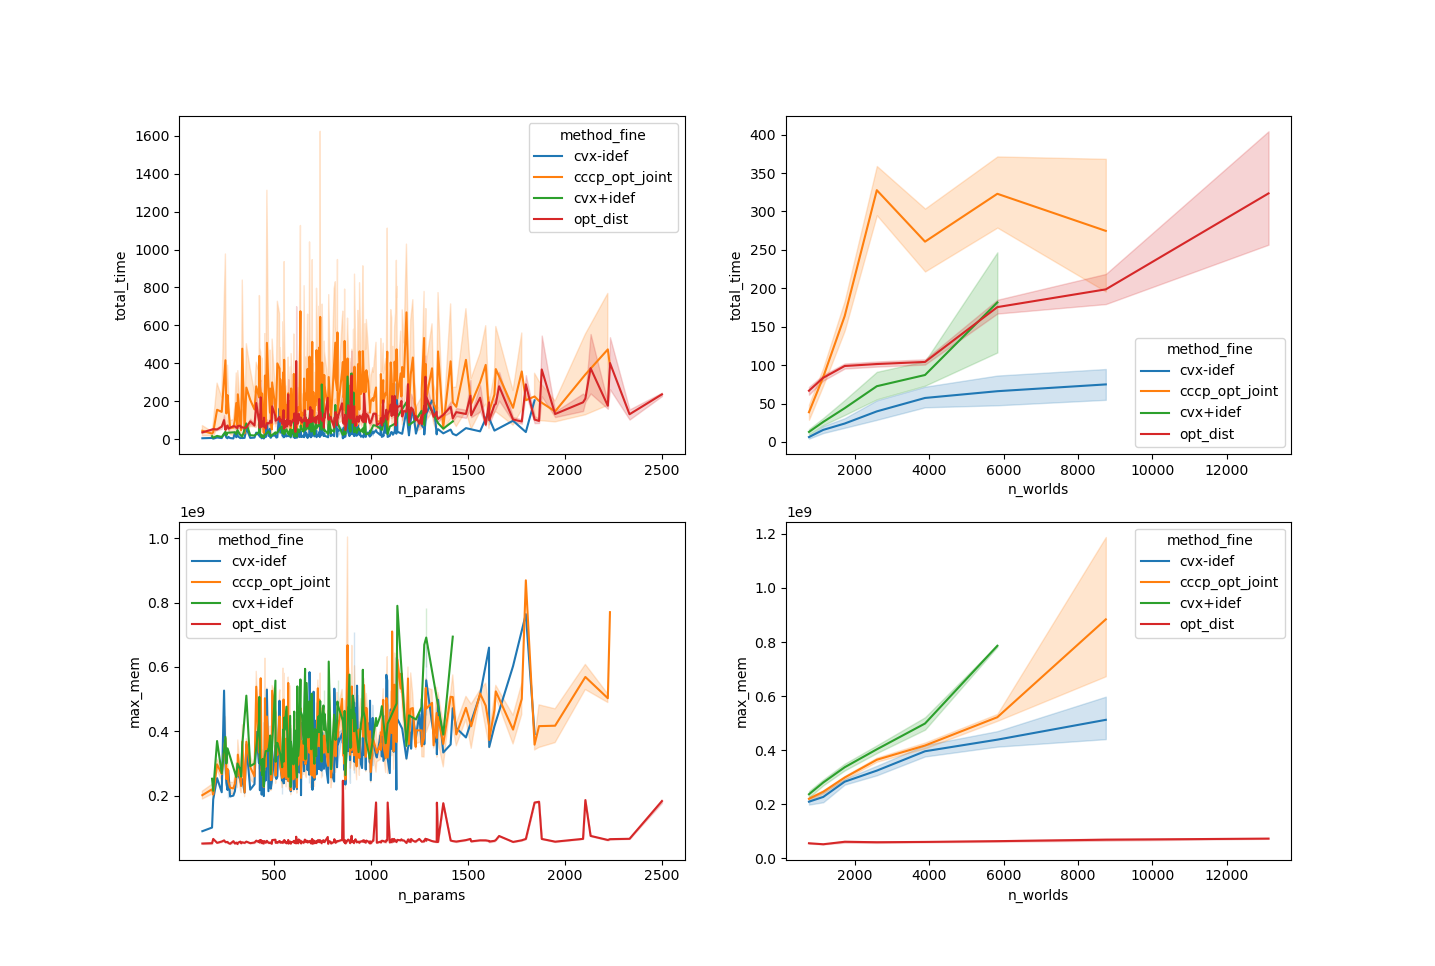
\includegraphics[width=\linewidth]{figs/resources-fine}
    \caption{
        The amount of resources: computation time (top) and maximum memory usage (bottom) for the various optimization methods (by color), as the size of the PDG increases, as measured by \texttt{n\_worlds} (right) and \texttt{n\_params} (left).
     }\label{fig:resources}
\end{figure}

\begin{figure}
    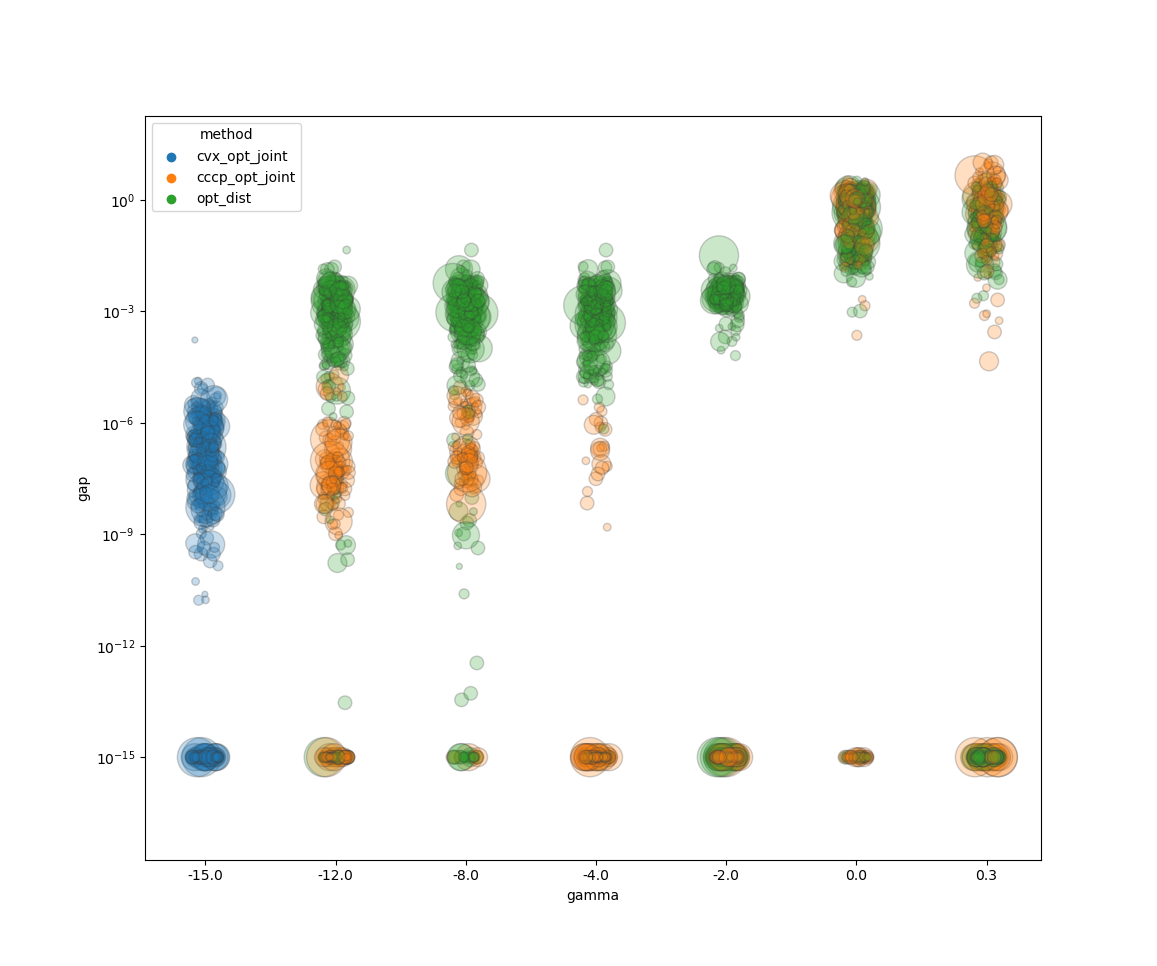
\includegraphics[width=\linewidth]{figs/gamma-vs-gap-bettergap}
    \caption{
        A graph of the gap (the difference between the attained objective value, and the best objective value obtained across all methods for that value of $\gamma$),
        as $\gamma$ varies. As before, colors indicate method.
        The size of the circle illustrates the relative number of worlds.
    }\label{fig:gamma-v-gap}
\end{figure}


\begin{figure}
    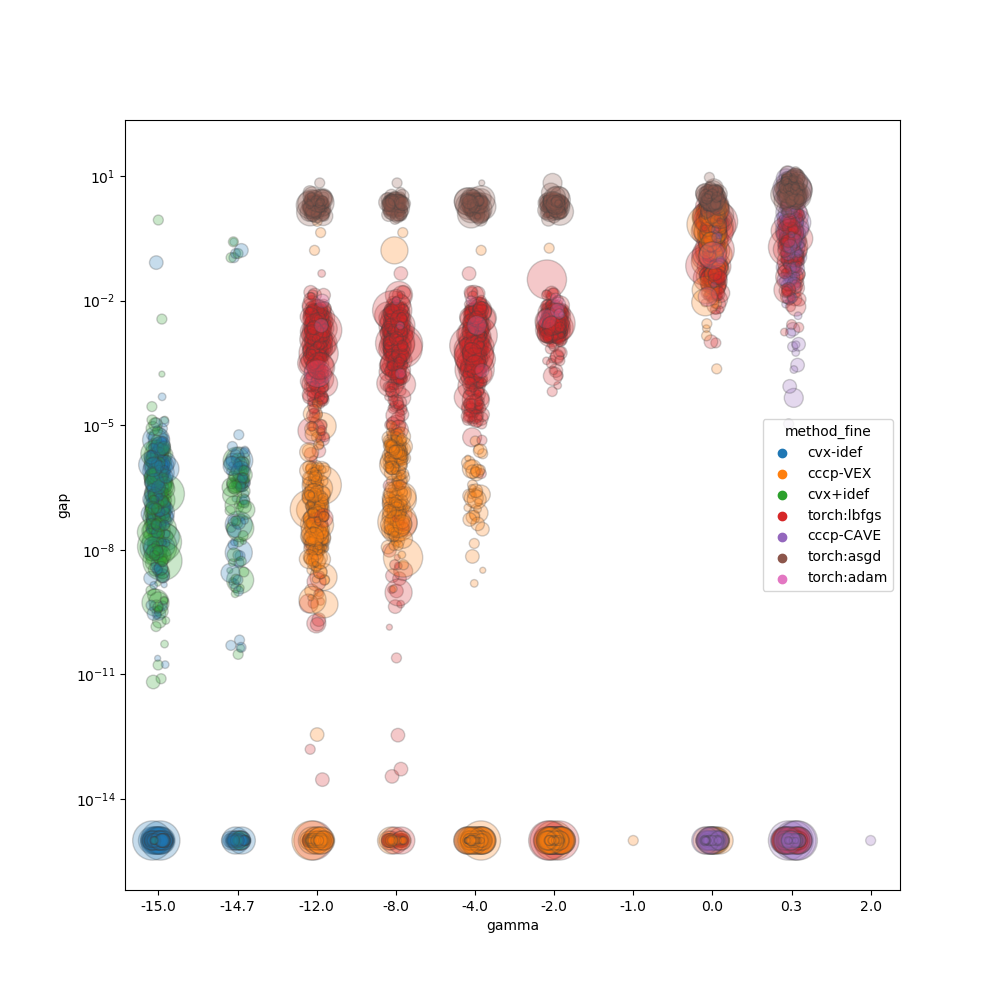
\includegraphics[width=\linewidth]{figs/2}
    \caption{
        A fine-grained variant of \cref{fig:gamma-v-gap}, which splits each method into sub-groups.
        The ExpCone methods \texttt{cvx\_opt\_joint} are split into two variants, depending on whether or not it also computed the second step described in \cref{sec:also-idef} to account for $\CDef_{}$.
        The CCCP variants are \texttt{cccp\_opt\_joint} split into regimes where the entire problem is convex, and the entire problem is concave. The optimization approaches \texttt{opt\_dist} are split into three different optimizers: LBFGS, Adam, and accelerated Gradient Descent.
    }\label{fig:gamma-v-gap-fine}
\end{figure}

\begin{figure}
    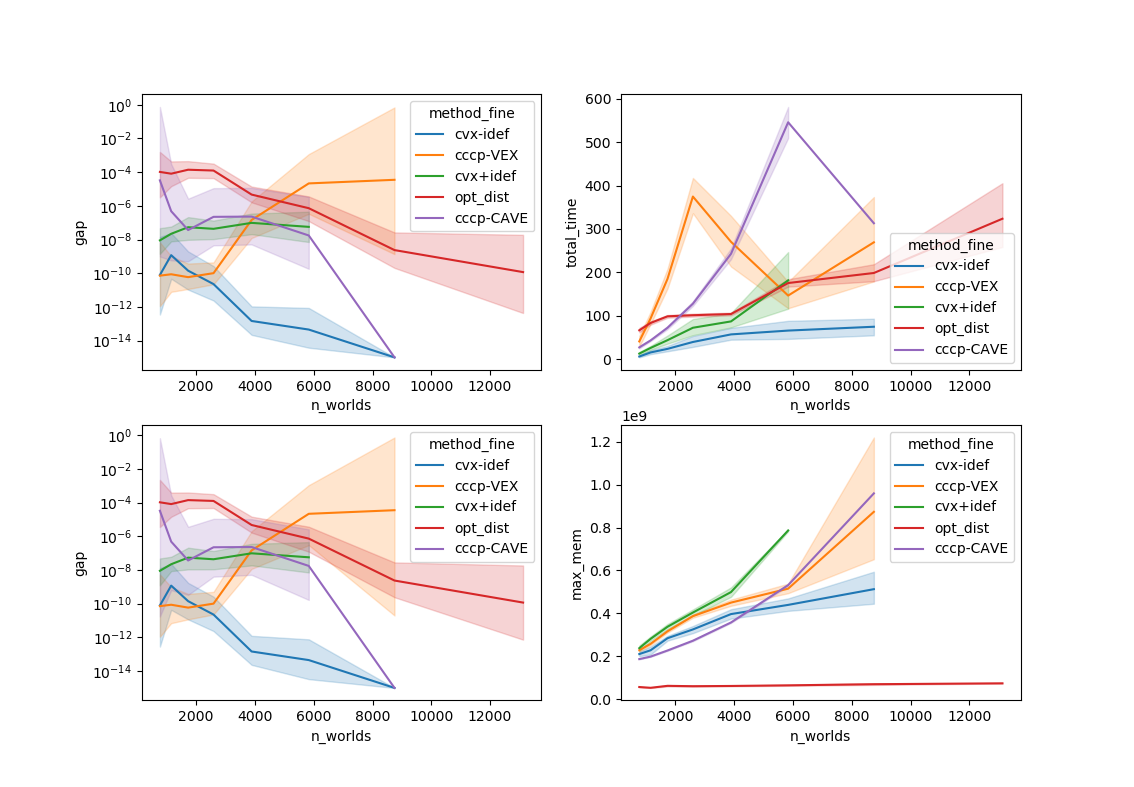
\includegraphics[width=\linewidth]{figs/1}
    \caption{
        A fine-grained variant of the right half of \cref{fig:resources},
        with gap information on the left.
    }\label{fig:gap-resource-fine}
\end{figure}


\begin{figure}
    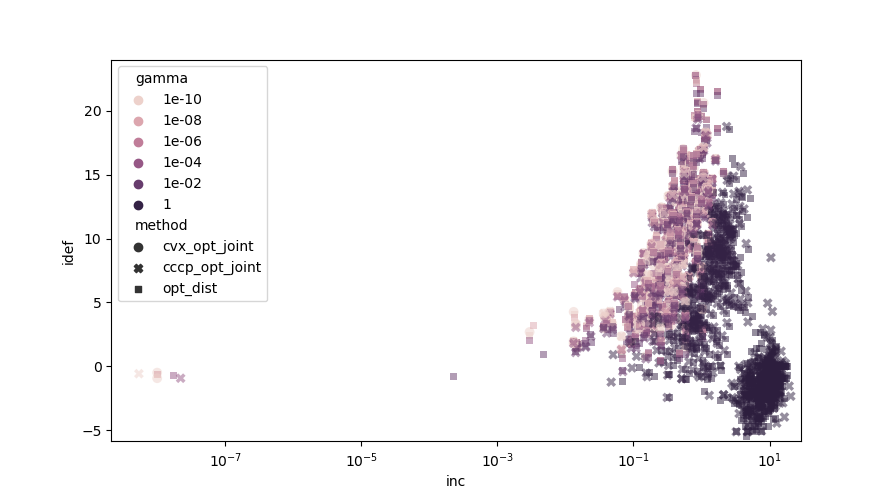
\includegraphics[width=\linewidth]{figs/inc-idef2}
    \caption{An illustration of the trade-off between $\OInc$ and $\CDef_{}$. Darker collors correspond to larger $\gamma$.}\label{fig:inc-idef}
\end{figure}

\subsection{Comparison To Belief propagation}

Since PDGs generalize other graphical models, one might wonder how our method stacks up against them.
We benchmarked against the small networks, and some of the medium-sized ones, from the \href{https://www.bnlearn.com/bnrepository/}{\texttt{bnlearn}} repository.



\subsection{Evaluations On Random PDGSs}
We start by focusing on empirical properties of the optimization over joint distributions.

We generated several hundred PDGs with various properties: 9 or 10 variables, each of which can take 2-3 values. Each PDG contains 7-15 hyperedges, with 1-2 target nodes and 0-3 source nodes. The cpds are chosen by taking uniformly random numbers from [0,1] and normalizing appropriately, and every $\beta$ is set to 1.
For each PDG $\dg M$, we measure its complexity by:
\begin{itemize}[nosep]
    \item \texttt{n\_edges}, the number of edges in $\dg M$,
    \item \texttt{n\_params}, the total number of parameters across all the cpds of $\dg M$, and
    \item \texttt{n\_worlds}, the size of the joint distributions on the variables of $\dg M$.
\end{itemize}

\textbf{Capacity.}
The black-box py-torch based approaches clearly have an edge in that they can handle larger models; see the cut-offs on the right sides of \cref{fig:resources,fig:gap-resource-fine}.

\textbf{Resource Costs.}
Look at \cref{fig:resources}.
Note that the exponential cone methods without the CCCP (blue and green) are actually faster than LBFGS, which was the best-performing torch optimizer.
However, they use \emph{significantly} more memory, and cannot handle more than 8000 worlds.


\textbf{Accuracy.}
In addition to being faster, the exponential cone techniques are also more preicse.
Note that the CCCP is typically more precise than the black-box optimizers when the problem is fully convex $\gamma \le 1$, and mirrors the performance of the exp-cone algorithms for the quantitative limit on the left, in blue.  For combinations of larger $\gamma$ and more worlds however, the 20 iteration maximum we imposed is not nearly enough to get convergence, and the black-box optimizers are both faster and attain better objective values.
\section{OTHER APPROACHES TO PDG INFERENCE} \label{sec:other-inference}
% \section{EXTENSIONS}


\subsection{}
A stronger result than \cref{prop:markov-property} holds as well.
\begin{prop}\label{prop:same-set-dists}
    % For all $\gamma > 0$ and in the limit as $\gamma \to 0$,
    Let $\Ed$ be a set of (hyper)edges over $\X$.
    For every PDG $\dg M$ over $\X$ with edges $\Ed$, every $\gamma > 0$, and every optimum $\mu^* \in \bbr{\dg M}_\gamma^*$ of $\dg M$'s scoring function at $\gamma$,
    there is a factor graph $\Phi$ with factors along $\Ed$ such that $\Pr_\Phi = \mu^*$.
\end{prop}

In other words: every distribution that a PDG can pick out as optimal (for any choice of $\gamma > 0$ and also in the limit as $\gamma \to 0$), can also be described as a factor graph with the same structure as that PDG.
How do we square this with the \citeauthor{pdg-aaai}'s claim that PDGs are more general than factor graphs?

% This may be surprising, given how \citeauthor{pdg-aaai} position their model as strictly more expressive than other graphical models, because it implies that the optimal distribution
\TODO[TODO: answer this question.\\
    The short answer: PDGs still compose differently, and in a way that respects the meaning of the probabilities. And just because you can find a factor graph that would have given you the right distribution after the fact, doesn't mean you could have specified the component factors.]
% The answer is simply that


\TODO[Also: don't get lost; figure out how to continue as below:]
\cref{prop:same-set-dists} suggests another approach to avoiding an exponential representation of $\mu$: given a PDG, fit a factor graph that has the same structure to it.

\subsection{Approximate Inference}
% \subsubsection{Relaxing the Marginal Polytope}
\textbf{Relaxing the marginal polytope.}
Just as it is possible to do belief propagation on cluster graphs that are not trees (e.g., loopy belief propagation)
so too is it possible to drop the requirement that the cluster that we use is indeed a tree decomposition.
This program is smaller, and will converge, but it will only be an approximate solution.
Like the original PDG itself, it might be inconsistent.

\subsubsection{Variational Approaches}

% Because of the deep connection between variational approaches
% shown in \parencite{one-true-loss}, there's





\section{DISCUSSION}

% Our anaysis
Our analysis shows that inference in PDGs with bounded tree-width can be done .


% \TODO[ the below is a transplant without context; fix it ]
% % Some queries are more difficult than others.
% Although we the question the same way, we also want to point out that there are other reasonable ways to answer that question once we move to PDGs.
% Suppose we were looking at a BN in which it just so happens that $\mat X$ contains only a single variable and $\mat Y$ are the parents of $\mat X$.
% In this case, our representation already contains the probabilities we are looking for, and we would be happy returning that row of the conditional probability table.
% But in a PDG, that cpd $p(\mat Y \,|\,\mat X)$, even if it is the only one
% attached to an edge from $X$ to $Y$, may not be the same as $\bbr{\dg M}^*(Y|X)$.
% As a consequence,


There are still a number of open questions.
\begin{itemize}
    \item What if $\bbeta < \gamma \balpha$?
\end{itemize}



\subsubsection*{Acknowledgements}
% All acknowledgments go at the end of the paper, including thanks to reviewers who gave useful comments, to colleagues who contributed to the ideas, and to funding agencies and corporate sponsors that provided financial support.
% To preserve the anonymity, please include acknowledgments \emph{only} in the camera-ready papers.

\subsubsection*{References}
\printbibliography


\clearpage
\onecolumn
\appendix
\section{Proofs}

\begin{lemma}
    For $\mat c \in \Rext^{3n}$, $\mat b \in \Rext^m$, and $\mat A \in \Rext^{m \times 3n}$,
    the exponential conic program
    % \eqref{eq:exp-conic-program}
    \[
        \mathop{\text{\sf minimize}}\limits_{\mat x \in \Rext^{3n}}~~ \mat c^{\sf T} \mat x
        \quad\text{\sf subject to}~~ \mat A \mat x = \mat b,~~\mat x \in K_{\exp}^n
        \tag{\ref{eq:exp-conic-program}}
    \]
    can be 
    \sout{solved to machine precision}
    {\color{red} solved to precision $\epsilon$ in some sense?},
    in $O(n (m+n)^{2.332}
    $\sout{$
    \log(m+n)
    $}$
    {\color{red} \log\nicefrac1\epsilon}
    )$ time. 
\end{lemma}
\begin{lproof}
    For this, we step through the algorithm and analysis of
     \textcite{badenbroek2021algorithm}, threading details through for the specific case
    where the conic constraint is $K_{\exp}^n$.
    
    % First, we'll need quite a few definitions.
    First, some of their definitions.
    A \emph{logarithmically homogeneous self-concordant barrier} with parameter $\nu$ ($\nu$-LHSCB) for a cone $K$ is a thrice differentiable strictly convex function $F: \mathrm{int}\, K \to \mathbb R$ satisfying
    $F(tx) = F(x) - \nu \log t$
    for all $t > 0$ and $x \in \mathrm{int}\, K$. 
    
    % Consider a point $\mat x = (\mat x_1, \mat x_2, \mat x_3) \in K_{\exp}^n$, 
        % where $\mat x_1, \mat x_2, \mat x_3 \in \mathbb R^{n}$. 
    % Consider a point $\mat x = 
    % (x^1_1, \ldots, x_n^1, x^2_1, \ldots, x^2_n, x^3_1, \ldots, x^3_n) 
    % (x_1^1, x_2^1, x_3^1, \ldots, x_1^n, x_2^n, x_3^n) 
    % \in K_{\exp}^n$.
        % where $\mat x_1, \mat x_2, \mat x_3 \in \mathbb R^{n}$. 
    
    We now take a break from their presentation to fill in some background facts about exponential cones.
    The \emph{dual} the exponential cone is
    % https://www.seas.ucla.edu/~vandenbe/236C/lectures/conic.pdf, slide 25. 
    \begin{align*}
        K_{\exp}^* &:= \{ (s_1, s_2, s_3) \in \mathbb R^3 : 
            x_1 s_1 + x_2 s_2 + x_3 s_3 \ge 0 \, \forall (x_1, x_2, x_3) \in K_{\exp} \}\\
            &= \{
                (s_1, s_2, s_3) : - s_1 \log (- s_1 / s_3) + s_1 - s_2 \le 0, s_1 \le 0, s_3 \ge 0
            \}.
    \end{align*}
    Consider points $x = (x_1, x_2, x_3) \in K_{\exp}$. 
    The function 
    \begin{equation}
        F_{\exp}(x) := - \log \Big(x_2 \log\frac{x_1}{x_2} - x_3\Big) - \log x_1 x_2
        % F(\mat x) := \sum_{i=1}^{n}
            % - \log \Big(x_2^i \log\frac{x_1^i}{x_2^i} - x_3^i\Big) - \log x_1^i x_2^i
        % F(\mat x) := - \log \Big(\mat x_2 \odot \log\frac{\mat x_1}{\mat x_2} - \mat x_3\Big) - \log (\mat x_1 \odot \mat x_2)
    \end{equation}
    % is a $3n$-LHSB for $K_{\exp}^n$, since
    is a $3$-LHSCB for $K_{\exp}$, since
    \begin{align*}
        F_{\exp}(t x) &= 
            -\log \Big( t x_2 \log \frac{t x_1}{t x_2} - t x_3\Big) - \log(t^2 x_1 x_2) \\
            % \sum_{i=1}^{n} - \log \Big( t x_2^i \log \frac{t x_1^i}{t x_2^i} - t x_3^i\Big) - \log(t^2 x_1^i x_2^i) \\ 
        % &= - \log \Big(t \big(\log \frac{x_1}{x_2} - x_3\big)\Big) - \log(x_1 x_2) - 2 \log t \\
        &= - \log \Big(t \big(\log \frac{x_1}{x_2} - x_3\big)\Big) - \log(x_1 x_2) - 2 \log t \\
        &= F_{\exp}(x) - 3 \log t
    \end{align*}
    Taking $n$ copies of a cone, and summning a $\nu$-LHSCB across each of the $n$ coordinates, results in a $3\nu$-LHSCB. In our case, this means that for $\mat x = (x^1, x^2, \ldots, x^n) \in K_{\exp}^n$ the function 
    $ F(\mat x) = \sum_{i=1}^n F_{\exp}(x^i) $
    is a $3n$-LHSCB for $K_{\exp}^n$, since
    $F(t \mat x) 
    = \sum_{i=1}^n F_{\exp}(t x^i)
    = \sum_{i=1}^n (F_{\exp}(x^i) - 3 \log t)
    = F(\mat x) - 3n \log t$. 
    $F$ can be evaluated in $O(n)$ time, and
    its gradient $F'(\mat x)$ and Hessian $F''(\mat x) \in \mathbb R^{3n \times 3n}$ at $\mat x$ can be expressed analytically.
    % $9n^2$ entries.
    Note that the latter has $(3n)^2$ entries. 
    Furthermore, the convex conjugate of $F$, given by 
    \begin{align*}
        F_*(s) &:=  
        % \sup_{x \in \mathrm{int}\, K_{\exp}^n} \{ - s^{\sf T} x- F(x) \}
        \sup\{ - s^{\sf T} x- F(x) : x \in \mathrm{int}\, K_{\exp}^n \}
            \\
        &= ???
    \end{align*}
    also has a known analytic form.
    
    \textcite{badenbroek2021algorithm} then define what they call \emph{shadow iterates}
    \[
        \tilde x := -F'_*(s)
        \qquad \text{and} \qquad
        \tilde s := - F'(x).
    \]
    which can be computed in in $O(n)$ time. 
    
    % The development requires a
    The primary object of study is a
    linear operator, called the \emph{homogenous self-dual} model,
    \[
        G(y,x,\tau,s,\kappa)
            := \begin{bmatrix}
                0          &  A  &  -b \\
                -A^{\sf T} &  0  &  c \\
                b^{\sf T}  & -c^{\sf T} & 0
        \end{bmatrix}
        \begin{bmatrix}
            y \\ x \\ \tau
        \end{bmatrix}
        -
        \begin{bmatrix}
            0 \\ s \\k
        \end{bmatrix}
    \]
    which is an $(3n+m+1)$-dimensional square matrix. 
    
    According to the MOSEK documentation [4]\parencite{MOSEKDOC},
        for the exponential cone,
    the algorithm initializes a guess
    \begin{align*}
        z_0 := (y_0, x_0, \tau_0, s_0, \kappa_0)
            \qquad
                \text{where}\quad
                x_0 &= s_0 = (1.291, 0.805, -0.828)^n \in 
                    (K_{\exp} \,\cap\, K_{\exp}^*)^n, \\
            \qquad
                y_0 &= \mat 0  \in \mathbb R^m,
            \quad
                \tau_0 = \kappa_0 = 1
    \end{align*}.
    
    \def\daff#1{\Delta {#1}^{\text{aff}}}
    \def\dcen#1{\Delta {#1}^{\text{cen}}}
    
    At each iteration, 
    we  will need to compute a scaling matrix
    \begin{equation}
        W :=
            \mu F''(x) + \frac{s s^{\sf T}}{\nu \mu}
            - \frac{\mu \tilde s \tilde s^{\sf T}}{\nu}
            + \frac{(s- \mu\tilde s)(s-\mu\tilde s)^{\sf T}}
                    {(s-\mu\tilde s)^{\sf T} (x - \mu \tilde x) }
            - \frac{\mu [ F''(x) \tilde x - \tilde \mu \tilde s]
                [ F''(x) \tilde x - \tilde \mu \tilde s]^{\sf T}}
                % { \Vert \tilde x \Vert^2_x - \nu \tilde \mu^2}
                { \tilde x^{\sf T} F''(x) \tilde x - \nu \tilde \mu^2}
        \label{eq:scalemat}
    \end{equation}
    Doing so requires $O(n^2)$ steps (although it may be parallelized). 
    The first four terms clearly require $O(n^2)$ steps, since each one is an outer product resulting in a $3n \times 3n$ matrix. 
    The last term computes a matrix-vector product (which requires $O(n^2)$ steps), and computes an outer product with the resulting vector, which takes $O(n^2)$ steps as well. 
    
    The next step involves finding a solution $\daff z = (\cdots)$
    to the system of equations
    \begin{subequations} \label{eqns:sys1}
    \begin{align}
        G(\daff z) &= -G(z) \\
        \tau \daff\kappa + \daff\tau &= - \tau \kappa \\
        W \daff x + \daff s &= -s
    \end{align}
    \end{subequations}
    
    This is a system of $(3n + m + 1) + 1 + (3n)$ equations and $3n + m + 1$ unknowns,
    which can be solved naively with Gaussian elimination in $O((n+m)^3)$ iterations,
    or with slightly better asymptotic complexity of
    $O((n+m)^{2.332})$.
    It may be possible to exploit the sparsity of $G$ to do slightly better. 
    
    The second half of the search direction is a solution $\dcen z$ to 
    \begin{subequations}\label{eqns:sys2}
    \begin{align}
        G(\dcen z) &= G(z) \\
        \tau \dcen \kappa + \kappa \dcen \tau &= \mu^e \\
        W \dcen x + \dcen s &= \mu^e \tilde s
    \end{align}
    \end{subequations}
    which again can be done in $O((n+m)^3)$ steps with Gaussian elimination, or
    with a fancier solver in $O((n+m)^2.332)$ steps. 
    
    The two updates are then applied to the current guess $z$ to obtain
    \[
        z_+ := z + \alpha (\daff z + \gamma \dcen z)
    \]
    
    Finally, a correction step $\Delta z_+^{\text{cor}}$
        is found by solving the system of equations
    \begin{subequations}\label{eqns:sys3}
    \begin{align}
        G(\Delta z^{\text{cor}}) &= 0 \\
        \tau_+ \Delta \kappa^{\text{cor}}  + \kappa_+ \Delta \tau^{\text{cor}} &= 0 \\
        W_+ \Delta {x_+}^{\text{cor}} + \dcen s &= \mu^e \tilde s
    \end{align}
    \end{subequations}
    where
    % \[
    %     W_+ :=
    %         \mu_+ F''(x_) + \frac{s s^{\sf T}}{\nu \mu}
    %         - \frac{\mu \tilde s \tilde s^{\sf T}}{\nu}
    %         + \frac{(s- \mu\tilde s)(s-\mu\tilde s)^{\sf T}}
    %                 {(s-\mu\tilde s)^{\sf T} (x - \mu \tilde x) }
    %         - \frac{\mu [ F''(x) \tilde x - \tilde \mu \tilde s]
    %             [ F''(x) \tilde x - \tilde \mu \tilde s]^{\sf T}}
    %             % { \Vert \tilde x \Vert^2_x - \nu \tilde \mu^2}
    %             { \tilde x^{\sf T} F''(x) \tilde x - \nu \tilde \mu^2}
    % \]
    $W_+$ is defined the same way as $W$, except that it uses the components of $z_+$ instead of $z$. 
    
    The full algorithm, then, is given as below:

    \begin{algorithmic}[1]
        % \State $z \gets (y_0, x_0, \tau_0, s_0, \kappa_0)$ as in \eqref{bbeq:init};
        \State $z \gets (y_0, x_0, \tau_0, s_0, \kappa_0)$;
        \While{}
            \State Compute scaling matrix $W$ as in \eqref{eq:scalemat};
            \State Find the solution $\daff z$ to (\ref{eqns:sys1}a-c),
                and the solution $\dcen z$ to (\ref{eqns:sys2}a-c);
            \State $z_+ \gets z + \alpha (\daff z + \gamma \dcen z)$;
            \State Compute the saling matrix $W_+$;
            \State Find the solution $\Delta z^{\text{cor}}_+$ to (\ref{eqns:sys3}a-c);
            \State $z \gets z_+ + \Delta z_+^{\text{cor}}$;
        \EndWhile
    \end{algorithmic}
    
    and each iteration of it takes $O((n+m)^{2.332})$ time. 
    Their main result \parencite[Theorem 3]{badenbroek2021algorithm}, states that for every $\epsilon \in (0,1)$,
    the algorithm results in a solution $z$ satisfying
    \[
        % \mu^e = 
        \frac{x^{\sf T} s + \tau \kappa}{3n + 1}
        \le \epsilon
        \qquad \text{and}\qquad
        \Vert G(z) \Vert \le \epsilon 
            % \Vert G(z_0) \Vert 
            \sqrt{3n + 1}
    \]
    in $O(3n \log (1/\epsilon))$ iterations, 
    for a total cost of 
    $O(n (m+n)^3 \log (1/\epsilon) )$ time with Gaussian elimination, or
    $O(n (m+n)^{2.332} \log (1/\epsilon) )$ time using the linear solver with best
         known asymptotatic complexity as of 2022.
         
    Finally,
     % to be within $\epsilon'$ of every component, 
    it suffices to set $\epsilon := 1/(m+n)$.
    
    \TODO[ In what sense is it converging at rate $\epsilon$? \\
        What makes it enough to get a machine-precision representation of the
        clique tree representing $\mu$?]

\end{lproof}

\recall{theorem:main}
\begin{lproof}\label{proof:main}
    
    Problem \eqref{prob:cluster-inc}
    has $\V\!\Ar + $ constraints.
    
    When translated via the DCP framework to 
    an exponential conic program of the form \eqref{eq:exp-conic-program}, 
    it has the original variables $\bmu$ and $\mat u$, as well as variables corresponding
    to each $[\mu_{C_{\!a}}(\Src a, \Tgt a)]$
    
\end{lproof}

\subsection{}

\recall{prop:smooth-and-strictly-cvx}
\begin{lproof}\label{proof:smooth-and-strictly-cvx}
	% First, we deal with the convexity, for which we make use of \cref{lem:cvx2}.
	% \commentout{
	% 	\def\mw#1{{\mat w}_{\!_{#1}}}
	% 	\def\ofmw(#1|#2){(\mw{#1} | \mw{#2})}
	% 	\begin{align*}
	% 		\aar{\dg M \bundle p}_\gamma &= \inf_\mu \Big[ \OInc_{\dg M \bundle p}(\mu)
	% 			+ \CDef_{\dg M \bundle p}(\mu) \Big] \\
	% 		&=  \inf_{\mu} \Ex_{\mat w \sim \mu}
	% 			\left[\log \mu(\mat w) +
	% 			 	\beta_p \log \frac{\mu\ofmw(Y|X)}{p\ofmw(Y|X)} \; +  \!\sum_{\ed LAB} \beta_L \log \frac{\mu\ofmw(B|A)}{\bp\ofmw(B|A)} + \alpha_L \log \frac{0}{\mu\ofmw(B|A)}\right] \\
	% 		&= f
	% 	\end{align*}
	% }
	We start by expanding the definitions, obtaining
	\begin{align*}
		\aar{\dg M \bundle p}_\gamma &= \inf_\mu ~\bbr{\dg M \bundle p}_\gamma(\mu) \\
			&= \inf_\mu \left[ \bbr{\dg M }_\gamma(\mu)
				+ \Ex_{x\sim\mu_{\!_X}} \kldiv[\Big]{\mu(Y\mid x)}{p(Y\mid x)} \right]\\
			&= \inf_\mu \left[ \bbr{\dg M }_\gamma(\mu)
				+  \kldiv[\Big]{\mu(X,Y)}{p(Y \mid X)\, \mu(X)} \right].
	\end{align*}
	% % Choose $\gamma < \min (\{1\}\cup\{ \beta^{\dg M}_L : L \in \Ed^{\dg M}\})$.
	% Since $\bbr{\dg M}_\gamma$ is a $\gamma$-strongly convex function of $\mu$ for all
	% such $\gamma < \min_L \beta_L$, and
	% $\kldiv{\mu_{XY}}{\mu_X \; p_{Y\mid X}}$ is 1-strongly
	% convex in $p$ for fixed $\mu$ (\cref{lem:Dstrongcvx}),
	% % $\thickD$ is convex in both of its arguments,
	% their sum is $\gamma$-strongly convex in $\mu$ and in $p$.
	% By \cref{lem:cvx2} taking an infemum preserves this convexity,
	% and so
	% $
	%  	\inf_\mu \left[ \bbr{\dg M }_\gamma(\mu)
	% 	+  \kldiv[\big]{\mu_{XY}}{p_{Y \mid X}\; \mu_X} \right]
	% $, which equals $\aar{\dg M \bundle p}_\gamma$,
	% is $\gamma$-strongly convex in $p$.
	% % $\aar{\dg M \bundle p}_\gamma$ is smooth
	% % Smoothness.


	% Choose $\gamma < \min (\{1\}\cup\{ \beta^{\dg M}_L : L \in \Ed^{\dg M}\})$.
	Fix $\gamma < \min_L \beta_L$. Then we know that $\bbr{\dg X}_\gamma(\mu)$ is a $\gamma$-strongly convex function for every PDG $\dg X$, and hence there is a unique joint distribution which minimizes it.

	\textbf{Strict Convexity.}
	Suppose $p_1(Y \mid X)$ and $p_2(Y\mid X)$ are two cpds on $Y$ given $X$.
	Fix $\lambda \in [0,1]$, and set $p_\lambda = (1-\lambda) p_1 + \lambda p_2$.
	Let $\mu_1, \mu_2$ and $\mu_\lambda$ be the joint distributions that minimze $\bbr{\dg M \bundle p_1}_\gamma$, $\bbr{\dg M \bundle p_2}_\gamma$ and $\bbr{\dg M \bundle p_\lambda}_\gamma$, respectively.  Then we have
	\begin{equation*}
		\aar{\dg M \bundle p_\lambda}_\gamma
			= \bbr{\dg M}_\gamma(\mu_\lambda) + \kldiv[\Big]{\mu_\lambda(X,Y)}{p_\lambda(Y\mid X) \mu_\lambda( X)}.
	\end{equation*}
	By convexity of $\bbr{\dg M}$ and $\thickD$, we have
	\begin{align}
		\bbr{\dg M}_\gamma(\mu_\lambda)
		 	&\le (\lambda-1)\bbr{\dg M}_\gamma(\mu_1) + \lambda \bbr{\dg M}_\gamma(\mu_2)
			 	\label{eqn:score-cvx}\\
		\text{and}\qquad \kldiv[\Big]{\mu_\lambda(XY)}{p_\lambda(Y | X) \mu_\lambda( X)}
			&\le (1-\lambda)\kldiv[\Big]{\mu_1(XY)}{p_1(Y | X) \mu_1( X)} \nonumber \\
			&\qquad+ \lambda\;\;\kldiv[\Big]{\mu_2(XY)}{p_2(Y | X) \mu_2( X)}.
				\label{eqn:D-cvx}
	\end{align}
	If $\mu_1 \ne \mu_2$ then since $\bbr{\dg M}$ is strictly convex, \eqref{eqn:score-cvx} must
	be a strict inequality. On the other hand, if $\mu_1 = \mu_2$, then since $\mu_\lambda = \mu_1 = \mu_2$ and $\thickD$ is stricly convex in its second argument when its first argument is fixed (\Cref{lem:Dstrongcvx}), \eqref{eqn:D-cvx} must be a strict inequality.
	In either case, the sum of the two inequalities must be strict, giving us
	\begin{align*}
		\aar{\dg M \bundle p_\lambda}_\gamma &=
		\bbr{\dg M}_\gamma(\mu_\lambda) + \kldiv[\Big]{\mu_\lambda(XY)}{p_\lambda(Y | X) \mu_\lambda( X)} \\
		&<
		 (\lambda-1) \left[\bbr{\dg M}_\gamma(\mu_1)
			 	+ \kldiv[\Big]{\mu_1(XY)}{p_1(Y | X) \mu_1( X)} \right]
			 \\[-0.3em]&\qquad\qquad
			 + \lambda \left[ \bbr{\dg M}_\gamma(\mu_2)
			 	+ \kldiv[\Big]{\mu_2(XY)}{p_2(Y | X) \mu_2( X)}
			 	\right] \\
		 &= (\lambda-1) \aar{\dg M \bundle p_1} + \lambda\,\aar{\dg M \bundle p_2},
	\end{align*}
	which shows that $\aar{\dg M \bundle p}$ is \emph{strictly} convex in $p$, as desired.


	\textbf{Smoothness.}
	If $\bbr{\dg M \bundle p}_\gamma^*$ is a positive distribution, then by definition $\bbr{\dg M \bundle p}$ achieves its minimum on the interior of the probability simplex $\Delta \V(\dg M \bundle p)$, and so by \Cref{lem:cvx4}, we immediately find that $\aar{\dg M \bundle p}_\gamma$ is smooth in $p$.

	Now, suppose that $\bbr{\dg M \bundle p}_\gamma^*(\mat w) = 0$,  for some $\mat w \in \V(\dg M \bundle p)$.

	Applying \Cref{lem:cvx4} to the function $f = \bbr{\dg M}_\gamma$

	Now for the second case.

	\TODO

	If $x^*_b \in \partial X$, then we claim that either
	\begin{enumerate}[nosep]
		\item There is a subspace $T \subseteq \mathbb R^{m}$ with
			$\SD{}$
	 	\item There is a subspace $S \subseteq \mathbb R^{n}$ with
			$x^*_b \in S \cap \partial X$ such

	\end{enumerate}

\end{lproof}

\begin{lemma}\label{lem:cvx4}
	Let $X$ and $Y$ be convex sets, and
	$f : X \times Y \to \mathbb R$ be a smooth $(C^\infty)$, convex function.
	If $f$ is strictly convex in $X$, and for some $y_0 \in Y$, $f(x, y_0)$ achieves its infemum on the interior of $X$.
	then $y\mapsto \inf_x f(x, y)$ is smooth $(C^\infty)$ at the point $y_0$.
\end{lemma}

\begin{lproof}%[Proof of \Cref{lem:cvx4}]
	% Let $f_y(x) = f(x,y)$.
	% Since $f$ is smooth and stritly convex, each restriction $f_y$ of $f$ to a
	% particular $y$ is also smooth and strictly convex.
	% As a result, each $f_y$ has a unique minimum $m_y := \inf_{x} f_y(x)$.
	% As $f_y$ is smooth, $m_y$ is either a boundary point, or
	% at a point where $\nabla f_y = 0$.
	%
	% Moreover, it is a constrained optimization problem, so
	% $\nabla_{x,y,\lambda} [ f(x,y) + \lambda (y_0 - y)] = 0$.
	%
	% \TODO
	Let $x_0^* := \arg\min_x f(x,y_0)$, which is achieved by assumption, and is unique because $f(-,y_0)$ is strictly convex.

	We will ultimately apply the implicit function theorem to give us a smooth function which is equal to this infemum, but to do so we must deal with the technicality that it requires an open set; the boundary is the most complicated part of this result.
	Here we have essentially required that the domain be open by fiat for $X$, but for $Y$ (which is a possibly non-open subset of $\mathbb R^m$), we use the Extension Lemma for smooth functions \cite[Lemma 2.26]{lee2013smooth}. In our context, it states that
	for every open set $U$ with $\overline{Y} \subseteq U \subseteq \mathbb R^m$,
	there exists a function $\tilde f : X \times \mathbb R^m \to \mathbb R$, such that $\tilde f |_{Y} = f$ (and $\supp \tilde f \subseteq U$).
	We only need a small fraction of this power: that we can smoothly extend $f$ to \emph{some} open set of $\mathbb R^m$, which we fix and call $\tilde Y$.

	% Similarly, for other $y \in Y$, let $x^*_y$ be the unique value of $x$ which minimizes $f(x,y)$.

	% \textbf{Smoothness.}
	% By assumption, $x^*_b$ is not a boundary point of $X$.
	%
	We claim that now all conditions for the Implicit Function Theorem are met if invoked with
		$\phi(y,x) := \vec\nabla_x \tilde f(x,y)$ and $(\mat b,\mat a) = (y_0, x^*_0)$.
	Concretely, we have $m = \mathop{dim} X$, $n = \mathop{dim} Y$, and $Z = (\tilde Y \times X)^\circ$, i.e., the interior of $\tilde Y \times X$, which is open and contains $(\mat b, \mat a)$.
	 Becuase $\phi$ is smooth, it is $k$-times differentiable for all $k$. We have $\vec\nabla_x \tilde f (y_0, x^*_0) = \vec 0$ because $x^*_0$ is a local minimum of the smooth function $\tilde f(-, y_0)$ which lies on the interior of $X$.

	Moreover, the Jacobian matrix
	\[ \mat J_{\nabla\!\tilde f, x}(y_0, x_0^*) = \left[ \frac{\partial^2 f}{\partial x_i \partial x_j}(x^*_0, y_0) \right]\]
	is the Hessian of the strictly convex funtion $f(-, b)$, and therefore positive definite (and in particular non-singular).
	Therefore, the Implicit Function Theorem guarantees us the existence of a neighborhood $U \subset \tilde Y$ of $y_0$ for which
	there is a unique $k$-times differentiable function $g: U \to X$ such that $g(y_0) = x^*_0$ and $\vec\nabla_x \tilde f(y, g(y)) = 0$ for all $y \in U$. Of course, this implies $g(y) = \argmin_x f(x,y)$ at every such point, and $\inf_x f(x,y) = f(g(y),y)$ is a composition of the smooth function $f$ with the $k$-times differentiable function $g \otimes \mathrm{id}_Y$.
	Therefore, $\inf_x f(x,y)$ is itself $k$-times continuously differentiable at $y_0$ for all $k$, or in other words, $\inf_x f(x,y)$ is smooth at $y=y_0$.
\end{lproof}

\recall{prop:markov-property}
\begin{lproof}
	Choose $\mu \in \bbr{\dg M_1 \bundle \dg M_2}^*_\gamma$.
	% Choose $\mu \in \mu^*_\gamma (\dg M_1 \bundle \dg M_2)$.
	Let $\mu' := \mu(\X_1) \mu(\X_2)$

	\TODO[Finish Transcribing Proof]
\end{lproof}


\subsection{Hardness Results}

\recall{prop:consistent-NP-hard}
\begin{lproof} \label{proof:consistent-NP-hard}
	We can directly encode SAT problems as PDGs.
	Specifically, let
	$$\varphi := \bigwedge_{j \in \mathcal J} \bigvee_{i \in \mathcal I(j)} (X_{j,i})$$
	be a CNF formula over binary variables $\mat X := \bigcup_{j,i} X_{j,i}$. Let
	$\dg M_\varphi$ be the PDG containing every variable $X \in \mat X$ and a binary
	variable $C_j$ (taking the value 0 or 1) for each clause $j \in \mathcal J$, as well as the following edges, for each $j \in \mathcal J$:
	%\{$``$\varphi(\mat X)$''$\}$ with $\V(\varphi) = \{0,1\}$, and
	\begin{itemize}
		\item a hyperedge $\{X_{j,i} : i \in \mathcal I(j)\} \tto C_j$, together with a degenerate cpd
			encoding the boolean OR function (i.e., the truth of $C_j$ given $\{X_{j,i}\}$);
		\item an edge $\pdgunit \tto C_j$, together with a cpd asserting $C_j$ be equal to 1.
	\end{itemize}
	% We give each edge $\alpha = 0$ and $\beta = 1$.
	First, note that the number of nodes, edges, and non-zero entries in the cpds are polynomial in the $|\mathcal J|, |\mat X|$, and the total number of parameters in a simple matrix representation of the cpds is also polynomial if $\mathcal I$ is bounded (e.g., if $\varphi$ is a 3-CNF formula).
	A satisfying assignment $\mat x \models \varphi$ of the variables $\mat X$ can be regarded as a degenerate joint distribution $\delta_{\mat X = \mat x}$ on $\mat X$, and extends uniquely to a full joint distribution $\mu_{\mat x} \in \Delta \V(\dg M_\varphi)$ consistent with all of the edges, by
	\[ \mu_{\mat x} = \delta_{\mat x} \otimes \delta_{\{C_j = \vee_i  x_{j,i}\}} \]

 	Conversely, if $\mu$ is a joint distribution consistent with the edges above, then any point $\mat x$ in the support of $\mu(\mat X)$ must be a satisfying assignment, since the two classes of edges respectively ensure that $1 =\mu(C_j\!=\! 1 \mid \mat X \!=\! \mat x) = \bigvee_{i \in \mathcal I(j)} \mat x_{j,i}$ for all $j \in \mathcal J$, and so $\mat x \models \varphi$.

	Thus, $\SD{\dg M_\varphi} \ne \emptyset$ if and only if $\varphi$ is satisfiable, so
	an algorithm for determining if a PDG is consistent can also be adapted (in polynomial space and time) for use as a SAT solver, and so the problem of determining if a PDG consistent is NP-hard.

% \end{lproof}
% \recall{prop:sharp-p-hard}
% \begin{lproof}\label{proof:sharp-p-hard}

    \medskip\hrule\smallskip

	\textbf{PART (b).}
    We prove this by reduction to \#SAT. Again, let $\varphi$ be some CNF formula over $\mat X$, and construct
	$\dg M_\varphi$ as in \hyperref[proof:consistent-NP-hard]{the proof} of
	\Cref{prop:consistent-NP-hard}.
	Furthemore, let $\bbr{\varphi} := \{ \mat x : \mat x \models \varphi \}$ be the set of  assingments to $\mat X$ satisfying $\varphi$, and $\#_\varphi := |\bbr{\dg M}|$ denote the number such assignments. We now claim that
	\begin{equation}\label{eqn:number-of-solns}
		\#_\varphi = \exp \left[- \frac1\gamma \aar{ \dg M_\varphi }_\gamma \right].
	\end{equation}
 	If true, we would have a reduced the \#P-hard problem of computing $\#_\varphi$ to the problem of computing $\aar{\dg M}_\gamma$ for fixed $\gamma$. We now proceed with proof \eqref{eqn:number-of-solns}.
	By definition, we have
	\[ \aar{\dg M_\varphi}_\gamma = \inf_\mu \Big[ \OInc_{\dg M_\varphi}(\mu) + \gamma \CDef_{\dg M_\varphi}(\mu) \Big]. \]
	We start with a claim about first term.
	% For the particular PDG $\dg M_\varphi$, the

	\begin{iclaim} \label{claim:separate-inc-varphi}
		% $\OInc(\dg M_\varphi)$ is finite if and only if $\varphi$ is statisfiable.
		$\OInc_{\dg M_\varphi}\!(\mu) =
		% \begin{cases}
		% 	0 & \text{if}~  \mat x \models \varphi~\text{and}~\mat c = \mat 1
		% 	 	~\text{for all}~(\mat x, \mat c) \in \supp \mu\\
		% 	\infty & \text{otherwise}
		% \end{cases}
		\begin{cases}
			0 & \text{if}~  \supp \mu \subseteq \bbr{\varphi} \times \{ \mat 1\} \\
			\infty & \text{otherwise}
		\end{cases}$.
	\end{iclaim}
	\vspace{-1em}
	\begin{lproof}
		Writing out the definition explicitly, the first can be written as
		\begin{equation}
			\OInc_{\dg M_\varphi}\!(\mu) = \sum_{j} \left[ \kldiv[\Big]{\mu(C_j)}{\delta_1} +
				\Ex_{\mat x \sim \mu(\mat X_j)} \kldiv[\Big]{\mu(C_j \mid \mat X_j = \mat x)}{\delta_{\lor_i \mat x_{j,i}}} \right], \label{eqn:explicit-INC-Mvarphi}
				% &= \sum_{j} \left[
				% 	\begin{matrix} \mu(C_j\!=\!0) (\infty) \\
				% 	 	+ \mu(C_j \!=\! 1) \log \mu(C_j \!=\! 1)
				% 	\end{matrix} +
				% 	\Ex_{\mat x \sim \mu(\mat X_j)} \kldiv[\Big]{\mu(C_j \mid \mat X_j = \mat x)}{\delta_{\lor_i \mat x_i}} \right],
		\end{equation}
		where $\mat X_j = \{X_{ij} : j \in \mathcal I(j)\}$ is the set of variables that
		appear in clause $j$, and $\delta_{(-)}$ is the probability distribution placing all mass on the point indicated by its subscript.
		As a reminder, the relative entropy is given by
		\[ \kldiv[\Big]{\mu(\Omega)}{\nu(\Omega)} := \Ex_{\omega \sim \mu} \log \frac{\mu(\omega)}{\nu(\omega)},
		\quad\parbox{1.4in}{\centering and in particular, \\ if $\Omega$ is binary,}\quad
			\kldiv[\big]{\mu(\Omega)}{\delta_\omega} = \begin{cases}
				0 &  \text{if}~\mu(\omega) = 1 ; \\
				\infty & \text{otherwise}.
		\end{cases} \]
		Applying this to \eqref{eqn:explicit-INC-Mvarphi}, we find that either:
		\begin{enumerate}[itemsep=0pt]
			\item Every term of \eqref{eqn:explicit-INC-Mvarphi} is finite (and zero) so $\OInc_{\dg M_\varphi}(\mu) = 0$, which happens when $\mu(C_j = 1) = 1$ and $\mu(C_j = \vee_i~ x_{j,i}) = 1$ for all $j$.  In this case, $\mat c = \mat 1 = \{ \vee_i~x_{j,i} \}_j$ so $\mat x \models \varphi$ for every $(\mat{c,x}) \in \supp \mu$;
			\item Some term of \eqref{eqn:explicit-INC-Mvarphi} is infinite, so that $\OInc_{\dg M_\varphi}(\mu) = \infty$, which happens if some $j$, either

			\begin{enumerate}
				\item $\mu(C_j \ne 1) > 0$ --- in which case there is some $(\mat{x,c}) \in \supp \mu$ with $\mat c \ne 1$, or
				\item $\supp \mu(\mat C) = \{\mat 1\}$, but $\mu(C_j \ne \vee_i~ x_{j,i}) > 0$ --- in which case there is some $(\mat{x,1}) \in \supp \mu$ for which $1 = c_j \ne \vee_i~x_{j,i}\;$, and so $\mat x \not\models \varphi$.
			\end{enumerate}
		\end{enumerate}
		Condensing and rearranging slightly, we have shown that
		\[
			\OInc_{\dg M_\varphi}(\mu) =
			\begin{cases}
				0 & \text{if}~  \mat x \models \varphi~\text{and}~\mat c = \mat 1
				 	~\text{for all}~(\mat x, \mat c) \in \supp \mu\\
				\infty & \text{otherwise}
			\end{cases}~.
		\]
		% So if $\mat x \models \varphi$ for all $\mat x \in \supp \mu(X)$,
		%
		% $\OInc_{\dg M_\varphi}(\mu) = 0$
		% The first term is infinite if $\mu(C_j = 1) < 1$, and the second is infinite
		% if $\mu(C_j = \lor_i X_{i,j}) < 1$. Thus, if $\OInc_{\dg M_\varphi}(\mu)$ is finite, then $\mat x \sim \mu(\mat X)$ satisfies $\varphi$ with probability 1, and $\varphi$ must be satisfiable.
		% Conversely,
	\end{lproof}

	% Thus, if $\OInc_{\dg M_\varphi}(\mu)$ is finite, then every $\mat x \in \supp \mu$ is a satisfying assignment of $\varphi$.
	Because $\CDef_{}$ is bounded, it follows immediately that
 	$\aar{\dg M_\varphi}_\gamma$, is finite if and only if
	there is some distribution $\mu \in \Delta\V(\mat X,\mat C)$ for which $\OInc_{\dg M_\varphi}(\mu)$ is finite, or equivalently, by \Cref{claim:separate-inc-varphi}, iff there exists some $\mu(\mat X) \in \Delta \V(\mat X)$ for which $\supp \mu(\mat X) \subseteq \bbr{\varphi}$, which in turn is true if and only if $\varphi$ is satisfiable.

	In particular, if $\varphi$ is not satisfiable (i.e., $\#_\varphi = 0$), then $\aar{\dg M_\varphi}_\gamma = +\infty$, and
	\[
		\exp \left[ -\frac1\gamma \aar{\dg M_\varphi}_\gamma \right] =
	 		\exp [ - \infty ] = 0 = \#_\varphi,
	\]
	so in this case \eqref{eqn:number-of-solns} holds as promised. On the other hand, if $\varphi$ \emph{is} satisfiable, then, again by \Cref{claim:separate-inc-varphi}, every $\mu$ minimizing $\bbr{\dg M_\varphi}_\gamma$, (i.e., every $\mu \in \bbr{\dg M_\varphi}_\gamma^*$) must be supported entirely on $\bbr{\varphi}$ and have $\OInc_{\dg M_\varphi}\!(\mu) = 0$.  As a result, we have
	\[
		\aar{\dg M_\varphi}_\gamma =
			\inf\nolimits_{\mu \in \Delta \big[\bbr{\varphi} \times \{\mat 1\}\big]} \gamma\; \CDef_{\dg M_\varphi}(\mu) .
	\]
	A priori, by the definition of $\CDef_{\dg M_\varphi}$, we have
	\[
		\CDef_{\dg M_\varphi}(\mu) =
		 	- \H(\mu) + \sum_{j} \Big[ \alpha_{j,1} \H_\mu(C_j \mid \mat X_j)
						+ \alpha_{j,0} \H_\mu(C_j) \Big],
	\]
	where $\alpha_{j,0}$ and $\alpha_{j,1}$ are values of $\alpha$ for the edges of $\dg M_\varphi$, which we have not specified because they are rendered irrelevant by the fact that their corresponding cpds are deterministic. We now show how this plays out in the present case.
	Any $\mu \in \Delta\big[\bbr{\varphi} \times \{\mat 1\}\big]$ we consider has a degenerate marginal on $\mat C$. Specifcally, for every $j$, we have $\mu(C_j) = \delta_1$, and since entropy is non-negative and never increased by conditioning,
	$$
		0 \le \H_\mu(C_j \mid \mat X_j) \le \H_\mu(C_j) = 0.
	$$
	Therefore, $\CDef_{\dg M_\varphi}(\mu)$ reduces to the negative entropy of $\mu$.
	Finally, making use of the fact that the maximum entropy distribution $\mu^*$ supported on a finite set $S$ is the uniform distribution on $S$, and has $\H(\mu^*) = \log | S |$, we have
	\begin{align*}
		\aar{\dg M_\varphi}_\gamma &= \inf\nolimits_{\mu \in \Delta \big(\bbr{\varphi} \times \{\mat 1\}\big)} \gamma\; \CDef_{\dg M_\varphi}(\mu) \\
			&= \inf\nolimits_{\mu \in \Delta \big(\bbr{\varphi} \times \{\mat 1\}\big)} -\, \gamma\, \H(\mu) \\
			&= - \gamma\, \sup\nolimits_{\mu \in \Delta \big(\bbr{\varphi} \times \{\mat 1\}\big)}  \H(\mu) \\
			&= - \gamma\, \log (\#_\varphi),
	\end{align*}
	\hspace{1in}giving us
	$$
		\#_\varphi = \exp \left[- \frac1\gamma \aar{ \dg M_\varphi }_\gamma \right],
	$$
	as desired. We have now reduced \#SAT to computing $\aar{\dg M}_\gamma$, for $\gamma > 0$ and an arbitrary PDG $\dg M$, which is therefore \#P-hard.

    To show the same for $\gamma = 0$, it suffices to add an additional hyperedge pointing to all variables, and associate it with a joint uniform distribution, and confidence 1, resulting in a new PDG $\dg M_\varphi'$.
    Then, because this new edge's contribution to $\OInc_{\dg M}$
    equals $\kldiv{\mu}{\mathsf{Unif}(\X)} = \log |\V\!\X| - \H(\mu)$,
    we have
    \[
        \bbr{\dg M_\varphi'}_0(\mu)
            = \OInc_{\dg M_\varphi'}(\mu)
            = \bbr{\dg M_\varphi}(\mu) + \log | \V\!\X | - \H(\mu)
            = \bbr{\dg M_\varphi}_{1}(\mu) - \log |\V\!\X |.
    \]
    Since this is true for all $\mu$, we conclude that
    \[
        \aar{\dg M_\varphi'} = \aar{\dg M_\varphi}_1 - \log |\V\!\X| = -\log \big( |\V\!\X|\cdot \#_\varphi \big)
    \]
    so the two differ by a constant, and both compute the number of satisfying assignments to $\varphi$. So in general, computing $\aar{\dg M}$ is \#P-hard as well.
\end{lproof}



\section{INFERENCE VIA INCONSISTENCY MINIMIZATION}
    \label{sec:inf-via-inc}

\TODO[TODO: rewrite this assuming that the entire main paper is in scope, rather than
    as an alternate introduction to inference of PDGs]

We are now equipped to talk more technically about inference in PDGs.
% When working with traditional graphical models, the meaning is clear.
%k
Since PDG semantics are already given in terms of a scoring function,
% the obvious thing to do is to find a distribution that minimizes it.
the obvious thing to do is to find a distribution that minimizes it.
%joe2*: But what does this minimization have to do with the inference
%problem you defined above?
%oli2*: if you have a concrete joint distribution, computing marginal probabilities of it is trivial, and conditioning is not much harder. Did my additions help?
Such a distribution $\mu$ could straightforwardly be used to answer probabilistic queries \eqref{q:inf} and compute inconsistency.
% There are several immediate difficulties.
There are some immediate difficulties with this approach.
% We immediately run into some obstacles.
% There are some obstacles to this.


\begin{enumerate}[nosep, label=\textbf{D\arabic*.}]
    \item Even writing down a distribution $\mu$, let alone evaluating its score $\bbr{\dg M}_\gamma (\mu)$, or minimizing it, takes exponential time.

    \item Generally speaking, optimization is computationally difficult.
        Even our most powerful optimization techniques only provably find optima in certain special cases.
    Unfortunately, while standard optimization techniques seem to work in practice
%joe1: why don't the standard tools apply in our setting?
%oli1: the next sentence explains it: the standard tools require Lipshitz-ness or
% self-concordance. How can I write this more clearly, if I don't really want to go into
% either but still want to mention the names so that people know what doesn't work?
%  (actually, the way the optimizer works is by using a self-concordant barrier function,
%       which is realted, but we can't use self-concordance directly in the obvious way.)
%
%      (more-or-less; see \cref{sec:expts}), the standard theoretical
      (more or less; see \cref{sec:expts}), the standard theoretical
      tools do not apply in our setting.
        % and even if it can be
%joe2*: What does it even mean for a pdg to be strictly convex?
%oli2*: The scoring function is convex, in its argument $\mu$. Is this unclear from the wording? [[M]]_\gamma is the scoring function.
%oli2: adding wording to try to abdicate responsibility for motivation
        % Despite being strictly convex,
        To be technical: despite being strictly convex,
        %oli2: removing because I have too many duplicate citations.
        % \parencite[at least for small $\gamma$,][]{pdg-aaai},
        and even $C^\infty$ smooth,
%joe1: I have no idea what self-concordant means.  Unless you're sure
%that over 90% of AIStats folks will now, you must define it and
%explain why it's relevant.  At least I know what the Lipshitz
%condition is, but it couldn't hurt to explain that too.
%joe2*: You still need to explain these terms and MOTIVATE why we care
%about them.
%oli2: I don't really. I want this to be a passing remark for those who know about self-concordance (which I'd guess is 40% of AISTATS folks) and Lipshitz-ness (I'd guess > 95% of AISTATS), but I really don't wan't to make a big deal of either of these two things. They're not important to me, they're just the standard tools that I don't think work. What do you think I should do?
        in general $\bbr{\dg M}_\gamma$ seems to be neither Lipshitz nor self-concordant.
         % convex (in $\mu$, which is exponentially large),
    \item Even if we coulld easily find optimizers of the function $\bbr{\dg M}_\gamma$ for fixed $\gamma > 0$, it's still not obvious that this would allow us to calculate the unique limiting distribution $\bbr{\dg M}^*$.
\end{enumerate}

We will ultimately address each of these issues, but before we do so,
% let's start with a shift in perspective.
let's start by trying to do inference as
suggested in the final section of \textcite{pdg-aaai}, which meshes well with
the persepctive taken in \textcite{one-true-loss}.

%joe2*: As I said, this should already be in the intro
%oli2*: As I responded below with %oli1, I disagree because it doesn't pan out;
% it's just an interesting perspective. I think this is the right place for it.
The argument there is that one can do modeling as follows:
    represent all of the relevant information as cpds,
    form a PDG out of them, and
%joe2*: I'm lost.  What knobs do we have?  This comes out of the blue.
%oli2: in this case, just $p(Y|X)$, but I was trying to reerence the general approach
% of my first AISTATS paper, not talk about this in particular. I've done a minor
% tweak to the wording to try to make this clear.
    % play with the knobs you have to to minimize the resulting inconsistency.
    play with whatever knobs are available, so as to minimize the overall inconsistency.
% Well, we have a PDG $\dg M$, and we also have a candidate joint distribution $\mu$.
% What if we put them both on the same footing, in a new PDG, and measure its inconsistency?
%joe1
%It is not hard to show that the distribution any distribution $\mu$
%that minimizes this quantity must also satisfy $\mu \in \bbr{\dg
% It is not hard to show that any distribution
% that minimizes this quantity must be in $\bbr{\dg
  % M}_\gamma^*$. More generally,
Well, we have a PDG $\dg M$, and we wanted to know the probablility of $Y$ given $X$.
What happens if we extend $\dg M$ with a guess, say $p(Y|X)$, and then
%oli2: added, to address your concern below
alter $p$ so as to minimize inconsistency?
As hinted in \textcite{pdg-aaai},
this
%oli2: modified
% would indeed perform our inference task,
would indeed suffice for inference,
%oli2: also added
since the optimal value of $p(Y|X)$ would be the cpd we wanted.

%joe2*: What does this proposition have to  say about the inference
%task you defined earlier.  A priori, it doesn't look that closely related.
%oli2: did my additions above help?
\begin{linked}{prop}{optimalYgivenX}
	% \label{prop:optimalYgivenX}
	% For all $\dg M$, $X,Y\in\X^{\dg M}$, and $\gamma > 0$, we have that
    For all variables $X,Y$, and $\gamma > 0$,
	$$\displaystyle
		% \argmin_{p : X \to \Delta Y}
		\argmin_{p(Y|X)}\,
        \aar{\dg M + p}_\gamma =
		\Big\{ \mu(Y | X) :  \mu \in \bbr{\dg M}_\gamma^* \Big\}
	,$$
% \end{linked}
%
% In the limit of small $\gamma$, since there is only one such distribution,
% the expression beomes simpler.
%
% \begin{linked}{coro}{smallgammaopt}
%joe1: What's a "quantiative limit"?
%oli1: it's the limit as \gamma -> 0;
% I defined it when I defined [[M]]^*, and also it's not necessary
% to remember the worlds, because the symbols are sufficient to get the meaning.
and in the quantiative limit,
	$\displaystyle
		\bbr{\dg M}^*(Y | X)
	$ is the unique minimizer of the function
$
    p(Y|X) \mapsto \aar{\dg M + p}
$
% which  a conditional probability on $Y$ given $X$ into the PDG $\dg M$.
%joe1: I have no idea what you're trying to say here.  What does it
%mean that it "includes a conditional probability on $Y$ given $X$
%into the PDG"
%oli1: good point--- I'm not just adding ("includig") the new probability, but
% also measuring its inconsistency.
% which measures the inconsistency of
\end{linked}

%joe1*: The claim that we can use inconsistency to compute the
%marginal probability of somne (small) set of variables is an
%important part of the story of why inconsistency is important, and
%should have come *much* earlier (i.e., in the introduction)
%
%oli1: If this was what gave the reason we don't discuss it in the introduction
Consequently, if we are interested only in querying the marginal probability of some small subset $Y$ of variables conditioned on other ones $X$ (i.e., the usual form of a query to a graphical model), and we had an efficient way to estimate the inconsistency of a guess $p(Y|X)$ with the rest of the model, we would have successfully cleared obstacle \textbf{D1}.

% Since inference in other graphical models is already NP-hard,
% and the class of PDGs subsumes capture them, it should be no surprise
% that inference in PDGs is NP hard as well.
%
%
% One might imagine that \emph{resolving} the inconsistency is the hard part,
%     as opposed to noticing it.
% Might it easier to simply determine whether or not a PDG is inconsistent?

Since inference in other graphical models is already NP-hard,
and PDGs subsume them, it should come as no surprise
that inference in PDGs is NP hard as well.
%
Still, one might imagine that \emph{resolving} the inconsistency is the hard part,
    as opposed to noticing it.
Might it easier to simply determine whether or not a PDG is inconsistent?
% If this seems reasonable, you might suspect that this reformulation could increase the difficulty of optimization (\textbf{D2})---that we might lose the several nice properties we do have (strict convexity and smoothness)---but this concern turns out not to be substantiated.
%
%joe2: we don't need to try to get into the reader's head
%oli2: the problem is that it doesn't (clearly) increase the difficulty of the optimization, so "this could increase" is wrong. I only mean to suggest that one might suspect that.
If this were the case, one might imagine that the reformulation
could increase the difficulty of optimization (\textbf{D2});
%joe2: why do we care if we lose them.  We're trying to do inference.
%This is copletely unnmotivated.
%oli2: we're trying to find an optimal joint distribution, which is one
% first pass at inference. Is it better motivated now?
% might lose the several nice properties we do have (strict convexity
might we lose the nice properties we do have (strict convexity
%joe2
%and smoothness)---but this concern turns out not to be substantiated.
% and smoothness).  This turns not to be the case.
and smoothness)?  It turns out that we don't.

%joe2*: Again, why do we care about this result?  How does it fit into
%the story.
%oli2: smoothness and strict convexity means gradient descent with
% an infinitely small step size is guaranteed to find the unique optimum distribution.
% It fits into the story because functions with these properties are relatively easy to
% optimize. At the outset, we know inference is hard. We can ask ourselves: is it the
% difficulty of optimizing the function, or the difficulty of evaluating it? The answer is
% the latter.  How can I make this come through?
\begin{linked}{prop}{smooth-and-strictly-cvx}
	The map $p \mapsto \aar{\dg M \bundle p}_\gamma$ is smooth and
		strictly convex
        %for $\gamma$%
	% (concretely: all $\gamma$ less than $\min (\{1\}\cup\{ \beta^{\dg M}_L : L \in \Ed^{\dg M}\})$
    when $\gamma < \min \{1\} \cup \{\beta_L\}_{ L \in \Ed}$.
	% .
\end{linked}

Operationally, though, we still haven't made much progress, since
we still don't have an easy way to compute $\aar{ ~\cdot~ }_\gamma$.
% In \cref{sec:complexity}, we will see why.
This is because there isn't one.
% For now,

% \begin{linked}{prop}{consistent-NP-hard}\label{sharp-p-hard}
%     \begin{enumerate}[nosep,label={\rm{(\alph*)}}]
%     \item Deciding if $\dg M$ is consistent is NP-hard.
%     \item Computing $\aar{\dg M}_\gamma$ is \#P-hard, for all $\gamma > 0$.
%     \end{enumerate}
% \end{linked}
\recall{prop:consistent-NP-hard}

% Since inference in other graphical models is already NP-hard,
% and the class of PDGs subsumes capture them, it should be no surprise
% that inference in PDGs is NP hard as well.


\subsection{}
\TODO[TODO: merge the presentation below in, which is essentially a more refined version of the above.]

If $\dg M_1$ and $\dg M_2$ are two PDGs, we can take the dusjoint union of their arcs (and associated data) to get a new PDG, denoted $\dg M_1 + \dg M_2$,
which represents the combined information of both $\dg M_1$ and $\dg M_2$.

% Let's start by trying to do inference by inconsistency minimization.
% suggested in the final section of \textcite{pdg-aaai},
% which meshes well with the persepctive taken in \textcite{one-true-loss}.
% \textcite{one-true-loss} suggests a generic learning-flavored
\textcite{one-true-loss} proposes a general
approach to probabilistic modeling with PDGs: represent each piece of relevant information (including any data, priors, and also a current hypothesis model $h(Y|X)$) as a cpd with the appropriate confidence, and then ``train'' $h$ by minimizing the overall inconsistency of the PDG (say, by gradient descent).
% This approach
In concluding,
\textcite{pdg-aaai} suggest that such an approach
could yield an inference algorithm as well.
We prove that indeed this gives the right answer.
% and indeed, it works.
% this would indeed suffice for inference,
% since the optimal value of $h(Y|X)$ would be the cpd we wanted.
% It turns out that the
% This

\begin{linked}{prop}{optimalYgivenX}
% For all variables $X,Y$, and $\gamma > 0$,
For all $\gamma > 0$ and $X, Y \subseteq \X^{\dg M}$,
	$$\displaystyle
		% \argmin_{p : X \to \Delta Y}
		\argmin_{h(Y|X)}\,
        \aar{\dg M + h}_\gamma =
		\Big\{ \mu(Y | X) :  \mu \in \bbr{\dg M}_\gamma^* \Big\}
	,$$
% and in the empirical limit,
and
	$\displaystyle
		\bbr{\dg M}^*(Y | X)
	$ is the unique minimizer of the function
$
    h(Y|X) \mapsto \aar{\dg M + h}
$.
% meaning that
\end{linked}
% Even more encouraging, this optimization
Furthermore, this optimization problem is solved by
% gradient flow,
% (gradient descent with infinitesimal steps)
gradient descent with infinitesimal steps,
since:
\begin{linked}{prop}{}
    the function $h \mapsto \aar{\dg M + h}_\gamma$
    % is $C^\infty$ smooth
    is infinitely differentiable
    and strictly convex for small $\gamma$.
\end{linked}
%
% Consequently, if we are interested in
% querying the marginal probability of some small subset $Y$ of variables conditioned on other ones $X$ (i.e., the usual form of a query to a graphical model),
% Consequently, if we
% had an efficient way to calculate the inconsistency of a PDG,
% together with the rest of the model,
%
% This suggests that PDG inference
% Since inference in other graphical models is already NP-hard,
% and the class of PDGs subsumes capture them, it should be no surprise
% that inference in PDGs is NP hard as well.
%
So, given an oracle that computes the inconsistency of a PDG,
% it seems we could do inference in a way that does not scale with the rest of the model.
it seems likely that one could do inference in a way that scales with the size of the queried variables, but not with the model.
% One might imagine that \emph{resolving} the inconsistency is the hard part,
%     as opposed to noticing it.
% Might it easier to simply determine whether or not a PDG is inconsistent?
%
% One might imagine that \emph{minimizing} inconsistency is the hard part, as opposed to merely noticing it---%
% Might it easier to simply determine whether or not a PDG is inconsistent?
% It is not.
% It turns out that calculat
% but it turns out that simply calculating the degree of
% but this is not the case.
% One might imagine that \emph{minimizing} inconsistency is the hard part, as opposed to merely noticing it---%
% but it's just as difficult.
% And, it turns out that minimizing inconsistency
% It turns out that even just computing inconsistency is \#P-hard.
One problem is that we still can't provably find the optimal distribution with larger discrete steps.
There's also another, bigger problem: simply identifying inconsistency is just as hard as resolving it.



% \section{INFERENCE IN A PDG, AND THE COMPUTATION OF INCONSISTENY}
\section{WHAT IS INFERENCE? SUBTLETIES FOR PDGS}
% \section{PDG INFERENCE, AND COMPUTING INCONSISTENCY}

What does inference mean in a PDG?
How ought we to respond to a probabilistic query $Q(Y|X{=}x)$?
The answer is not so obvious as it is for other graphical models,
for several different reasons.

\textbf{1.}
% First,
PDGs describe inconsistent beleifs,
so why should we expect to get consistent answers by querying them?
% If the inconsistency were sorted out, then arguably there is no need for a PDG; one may use a probability distribution, or a compressed representation of one (such as a different graphical model) instead.
% Were we able to sort out the inconsistency,
% there is a case to be made that
Even for BNs, we often use algorithms that give inconsistent answers to queries, and BNs very clearly represent a single distribution.
%
% To illustrate one aspect of this,
% A BN may already contain answers to the querie
% Consider a BN in which $X$ is the set of parents of $Y$.
% In this case, our representation already contains the probabilities we are looking for, and we would be happy returning that row of the table.
% Such a BN has a row of a table that represents $\Pr(Y|X{=}x)$, which is the answer we are looking for.
In a BN, we might get lucky and find a row of a cpd that represents $\Pr(Y|X{=}x)$, which would be the answer we're looking for.
% and it would be reasonable to short-circuit an inference procedure upon finding it.
% But in a PDG, that same  $p(Y | X)$ may not even be the only conditional probability on $Y$ given $X$, let alone the same as $\bbr{\dg M}^*(Y|X)$.
% But in a PDG, that very same row  $p(Y | X{=}x)$ of the same table may not even be the only  let alone the same as $\bbr{\dg M}^*(Y|X)$.
But in a PDG, that same row  $p(Y | X{=}x)$ might not even be the only probability of $Y$ given $X{=}x$, let alone the same as $\bbr{\dg M}^*(Y|X)$.

\textbf{2.}
% \textbf{Conditioning.}
% Secondly,
% Here's a property of PDGs that is not shared by other graphical models:
% Unlike other graphical models,
% Unlike for other graphical models,
% there is a
% PDGs draw a distinction between constraining so that $X{=}x$,
% and  distribution.
In sharp contrast to other graphical models \parencite[pg 26]{koller2009probabilistic},
the PDG formalism draws a distinction between
% computing the distribution of $Y$ under the constraint $X{=}x$,
the posterior distribution of $Y$ after learning that $X{=}x$,
and computing the distribution of $Y$ given $X{=}x$, conditioned in the usual way.

\begin{example}
	Consider a PDG $\dg M$ containing $p(Y)$ with confidence
    $\beta_p = r$, and $q(X|Y)$ with confidence $\beta_q = s$.
	% Now condition on $Y=y$ by adding that event to the PDG, to get
    Now, add the event $X{=}x$ to $\dg M$, to obtain
    % a new PDG:
    a new PDG, $\dg M^{+x}$.
	% \[
	% 	\dg M^{+y} :=
	% 	\begin{tikzpicture}[center base]
	% 		\node[dpad0] (X) at (0,0) {$X$};
	% 		\node[dpad0] (Y) at (1.2,0) {$Y$};
    %         %
	% 		\draw[arr2,->] (X) to
	% 			node[above, pos=0.4,inner sep=2pt]{$q$}
	% 			node[below, pos=0.4, inner sep=2pt]{${\color{gray}\scriptstyle(s)}$}
	% 			(Y);
	% 		\draw[arr2, <-] (X) to
	% 			node[above, pos=0.6,inner sep=2pt]{$p$}
	% 			node[below, pos=0.6, inner sep=2pt]
	% 				{${\color{gray}\scriptstyle(r)}$}
	% 			+(-1.0, 0);
	% 		\draw[arr2, <<-, red] (Y) to
	% 			node[above, inner sep=2pt, pos=0.7]
	% 				{$y$}
	% 			+(0.9,0);
	% 	\end{tikzpicture}.
	% \]
	Now, $\bbr{\dg M}^* = p(Y)q(X|Y)$ doesn't depend on $r$ or $s$, since we can simultaneously satisfy $p$ and $q$---and after conditioning on $X{=}x$, we get a distribution $\bbr{\dg M}^* | X{=}x$ proportional to $p(Y) q(x|Y)$.
	But some calculations reveal that $\bbr{\dg M^{+x}}^*$,
    while also supported only on worlds where $X{=}x$, is proportional to
	$p(Y) q(x|Y)^{s/r}$.
    % , with an additional exponent $r/s$ that was not present before.
	%
	So if $r = s$,
    % so that the data of $\dg M$ effectively picks out a probability distribution with uniform confidence,
    this amounts to conditioning as usual, but otherwise,
    it doesn't.
    % there is distortion.
    % we don't.
    % Intuitively, the cpd with lower confidence ends
    Intuitively, both the distribution of $Y$ and the conditional distribution of $X$ given $Y$ can be bent to satisfy $X{=}x$, and in $\bbr{\dg M^{+x}}^*$ the cpd with lower confidence will be bent further than the one of higher confidence.
    If $r \gg s$ for example,
    % then the resulting distribution will just be
    then $\bbr{\dg M^{+x}}^* \approx
    % p(X)\delta_{y}(Y)$.
    p(Y) \delta_x(X)$.
    And perhaps that is even a better answer than conditioning, if indeed we are far more confident in $p$ than in $q$.
\end{example}

So, adding an event to a PDG is a different kind of conditioning,
which is sensitive to confidence.  This has big implications for responding to conditional probability queries, because it means there can be a big difference between restricting to worlds where $Y{=}y$, as is typically done, and conditioning on $Y{=}y$.
Because both notions are defensible,
we start with the uncontroversial, simpler version: solving the marginal inference task.
% So as not to privelidge either notion over the other,
% we define PDG inference to be the marginal task.
% Both notions are defensible, but to put them on the same footing.


% By inference in a PDG, we mean respoding to probabilisty qureies $Q(Y|X)$ for (sets of) variables $X,Y \subset \X$
\begin{defn}
    A \emph{marginal PDG inference algorithm} is a procedure
    that takes as input
    % (1)
    a PDG $\dg M$ over variables $\X$,
    % a non-negative number $\gamma \ge 0$ or $0^+$,
    % either a non-negative number $\gamma \ge 0$ or $\gamma = $``$0^+$'',
    % (2)
    a value for $\gamma \in \mathbb R_{\ge 0} \cup \{0^+\}$,
    and
    % (3)
    % a probabilistic query of the form $Q(Y|X{=}x)$,
    a set of variables $Y \subset \X$,
    % for $X,Y \subset \X$ and $x \in \V X$,
    % returns a probability distribution $\mu(Y)$ that is the conditional marginal
    % and then returns either a distribution $\mu(Y|X{=}x)$
    and then returns either a distribution $\mu(Y)$
    which is the
    % conditional
    marginal
    of some $\mu \in \bbr{\dg M}^*_\gamma$  (if $\gamma$ is a number),
    % or $\bbr{\dg M}^*(Y|X{=}x)$ (if $\gamma = 0^+$).
    or $\bbr{\dg M}^*(Y)$ (if $\gamma = 0^+$).
\end{defn}

We can use such marginal inference algorithm
to respond to \emph{conditional} probabilistic queries
% about of $Y$ given $X{=}x$
$Q(Y|X{=}x)$ in both ways.
% in at least two ways:
% one can run
% $\mathit{MInfer}$
On one hand, we can query the marginal distribution of $Y$ in $\dg M + (X{=}x)$
to get this new kind of conditioning;
% $\bbr{\dg M + X{=}x}_\gamma^*(Y) =
% $\mathit{InferMarg}_\gamma(Y | \dg M + (X{=}x) )$.
% That is, first adding the event $X{=}x$ to the PDG.
%
% This procedure can also be used to answer the question in the same way as for other graphical models with minimal overhead.
% Another way
% First, if $X$ is a small set of variables, then we can compute both the marginal $\mu(X,Y)$ and the marginal $\mu(X)$ and compute $\mu(Y|X{=}x)$ directly.
% Alternatively,
% Furthermore,
% On the other hand,
% it will $\mu^*(Y|X{=}x)$
on the other,
each method we present can be augmented with a standard post-procesing step
to compute the usual conditional probability $\mu^*(Y|X{=}x)$.
% can be computed with some post-processing.
% to a conditional probability query amounts to a standard postprocessing step,
% which does not significantly impact the complexity of the algorithm.



\section{LARGER
    \texorpdfstring{$\boldsymbol\gamma$}{GAMMA} AND THE CONVEX-CONCAVE PROCEDURE}
    \label{sec:larger-gamma}

% Now, suppose we're no longer
Next, let's consider the case where $\gamma$ is
larger, meaning that the structural term $(\CDef_{})$,
becomes more important.
Because $\CDef_{}$ can express features of a distribution like conditional indepenedence,
it cannot be convex.%
    \footnote{one can easily verify that set of distributions that make $X$ and $Y$ independent is not convex.}
Nevertheless, \eqref{eq:altscore} still gives us a way to proceed because it is a decomposition into a sum of a convex and a concave function, meaning that we can apply the convex-concave procedure, or CCCP \parencite{yuille2003concave}.
% The first line is the sum of a linear term and a convex one,
In more detail: and each individual term on the second line is either convex or concave, depending on the sign of the quantity $\gamma \alpha\ssub L - \beta\ssub L$.
Once we sort the terms into convex terms $f(\mu)$ and strictly concave terms $g(\mu)$, we can choose an initial guess $\mu_0$, and iteratively use the convex solver as in \cref{sec:small-gamma} to compute
%
\begin{align*}
    \mu_{t+1} &:= \argmin_{\mu} f(\mu) + (\mu - \mu_{t})^{\sf T}
        \nabla g(\mu_t)
\end{align*}

As we will see, the aproach presented here section is
not very fast, but it is guaranteed to make progress, since
\def\tplus1{{t\mskip-2mu+\mskip-2mu1}}
\begin{align*}
    f(\mu_\tplus1) \!+\! g(\mu_\tplus1) &<  f(\mu_\tplus1) \!+\! (\mu_\tplus1 \!-\! \mu_t)^{\sf T} \nabla g(\mu_t) \!+\! g(\mu_t)
        % &\text{(concavity of $g$)}
        \\
    &\le  f(\mu_t) + (\mu_t - \mu_{t})^{\sf T}\nabla g(\mu_t)  + g(\mu_t)
        % &\text{(defn of argmin)}
    \\
&= f(\mu_t) + g(\mu_t)
\end{align*}
and eventually find an optimum, because the concave terms are bounded (since they are conditional entropies of a finitely supported distribution).

\subsection{Experiments}


\section{}
\begin{conj}
    Inference in a PDG---that is, computing conditional marginals of $\bbr{\dg M}^*$---%
    and the computing inconsistency $\aar{\dg M}$ are equally difficult:
        there are polynomial-time reductions from each to the other.
\end{conj}

If we do not restrict to finite variables, then the problem is much worse.

\begin{linked}{conj}{incomputable}
    The problem of deciding whether a PDG whose variables take values in $\mathbb N$ is not computable.
\end{linked}

\end{document}
